%&preformat-disser
\RequirePackage[l2tabu,orthodox]{nag} % Раскомментировав, можно в логе получать рекомендации относительно правильного использования пакетов и предупреждения об устаревших и нерекомендуемых пакетах
% Формат А4, 14pt (ГОСТ Р 7.0.11-2011, 5.3.6)
\documentclass[a4paper,14pt,oneside,openany]{memoir}

%% Режим черновика
\makeatletter
\@ifundefined{c@draft}{
  \newcounter{draft}
  \setcounter{draft}{0}  % 0 --- чистовик (максимальное соблюдение ГОСТ)
                         % 1 --- черновик (отклонения от ГОСТ, но быстрая сборка итоговых PDF)
}{}
\makeatother

%% Использование в pdflatex шрифтов не по-умолчанию
\makeatletter
\@ifundefined{c@usealtfont}{
  \newcounter{usealtfont}
  \setcounter{usealtfont}{1}    % 0 --- шрифты на базе Computer Modern
                                % 1 --- использовать пакет pscyr, при его наличии
                                % 2 --- использовать пакет XCharter, при наличии подходящей версии
}{}
\makeatother

%% Библиография

%% Внимание! При использовании bibtex8 необходимо удалить все
%% цитирования из  ../common/characteristic.tex
\makeatletter
\@ifundefined{c@bibliosel}{
  \newcounter{bibliosel}
  \setcounter{bibliosel}{1}           % 0 --- встроенная реализация с загрузкой файла через движок bibtex8; 1 --- реализация пакетом biblatex через движок biber
}{}
\makeatother

%%% Предкомпиляция tikz рисунков для ускорения работы %%%
\makeatletter
\@ifundefined{c@imgprecompile}{
  \newcounter{imgprecompile}
  \setcounter{imgprecompile}{0}   % 0 --- без предкомпиляции;
                                  % 1 --- пользоваться предварительно скомпилированными pdf вместо генерации заново из tikz
}{}
\makeatother
               % общие настройки шаблона
%%% Проверка используемого TeX-движка %%%
\RequirePackage{ifxetex, ifluatex}
\newif\ifxetexorluatex   % определяем новый условный оператор (http://tex.stackexchange.com/a/47579)
\ifxetex
    \xetexorluatextrue
\else
    \ifluatex
        \xetexorluatextrue
    \else
        \xetexorluatexfalse
    \fi
\fi

\newif\ifsynopsis           % Условие, проверяющее, что документ --- автореферат

\RequirePackage{etoolbox}[2015/08/02]               % Для продвинутой проверки разных условий

%%% Поля и разметка страницы %%%
\usepackage{pdflscape}                              % Для включения альбомных страниц
\usepackage{geometry}                               % Для последующего задания полей

%%% Математические пакеты %%%
\usepackage{amsthm,amsmath,amscd}       % Математические дополнения от AMS
\ifxetexorluatex
    \usepackage{amsfonts,amssymb}       % Математические дополнения от AMS
\else
    \ifnumequal{\value{usealtfont}}{2}{}{
        \usepackage{amsfonts,amssymb}       % Математические дополнения от AMS
    }
\fi
\usepackage{mathtools}                  % Добавляет окружение multlined

%%%% Установки для размера шрифта 14 pt %%%%
%% Формирование переменных и констант для сравнения (один раз для всех подключаемых файлов)%%
%% должно располагаться до вызова пакета fontspec или polyglossia, потому что они сбивают его работу
\newlength{\curtextsize}
\newlength{\bigtextsize}
\setlength{\bigtextsize}{13.9pt}

\makeatletter
%\show\f@size                                       % неплохо для отслеживания, но вызывает стопорение процесса, если документ компилируется без команды  -interaction=nonstopmode 
\setlength{\curtextsize}{\f@size pt}
\makeatother

%%% Кодировки и шрифты %%%
\ifxetexorluatex
    \usepackage{polyglossia}[2014/05/21]            % Поддержка многоязычности (fontspec подгружается автоматически)
\else
   %%% Решение проблемы копирования текста в буфер кракозябрами
    \ifnumequal{\value{usealtfont}}{1}{% Используется pscyr, при наличии
        \IfFileExists{pscyr.sty}{% вероятно, без pscyr нет необходимости в этом коде
            \input glyphtounicode.tex
            \input glyphtounicode-cmr.tex %from pdfx package
            \pdfgentounicode=1
        }{}
    }{}
    \usepackage{cmap}                               % Улучшенный поиск русских слов в полученном pdf-файле
    \defaulthyphenchar=127                          % Если стоит до fontenc, то переносы не впишутся в выделяемый текст при копировании его в буфер обмена 
    \usepackage[T1,T2A]{fontenc}                    % Поддержка русских букв
    \ifnumequal{\value{usealtfont}}{1}{% Используется pscyr, при наличии
        \IfFileExists{pscyr.sty}{\usepackage{pscyr}}{}  % Подключение pscyr
    }{}
    \usepackage[utf8]{inputenc}[2014/04/30]         % Кодировка utf8
    \usepackage[english, russian]{babel}[2014/03/24]% Языки: русский, английский
    \ifnumequal{\value{usealtfont}}{2}{
        % http://dxdy.ru/post1238763.html#p1238763
        \usepackage[scaled=0.925]{XCharter}[2017/06/25] % Подключение русифицированных шрифтов XCharter
        \usepackage[bitstream-charter]{mathdesign} % Согласование математических шрифтов
    }{}
\fi

%%% Оформление абзацев %%%
\usepackage{indentfirst}                            % Красная строка

%%% Цвета %%%
\usepackage[dvipsnames, table, hyperref, cmyk]{xcolor} % Совместимо с tikz. Конвертация всех цветов в cmyk заложена как удовлетворение возможного требования типографий. Возможно конвертирование и в rgb.

%%% Таблицы %%%
\usepackage{longtable,ltcaption}                    % Длинные таблицы
\usepackage{multirow,makecell}                      % Улучшенное форматирование таблиц

%%% Общее форматирование
\usepackage{soulutf8}                               % Поддержка переносоустойчивых подчёркиваний и зачёркиваний
\usepackage{icomma}                                 % Запятая в десятичных дробях
\usepackage[hyphenation, lastparline]{impnattypo}   % Оптимизация расстановки переносов и длины последней строки абзаца

%%% Гиперссылки %%%
\usepackage{hyperref}[2012/11/06]

%%% Изображения %%%
\usepackage{graphicx}[2014/04/25]                   % Подключаем пакет работы с графикой

%%% Списки %%%
\usepackage{enumitem}

%%% Счётчики %%%
\usepackage[figure,table]{totalcount}               % Счётчик рисунков и таблиц
\usepackage{totcount}                               % Пакет создания счётчиков на основе последнего номера подсчитываемого элемента (может требовать дважды компилировать документ)
\usepackage{totpages}                               % Счётчик страниц, совместимый с hyperref (ссылается на номер последней страницы). Желательно ставить последним пакетом в преамбуле

%%% Продвинутое управление групповыми ссылками (пока только формулами) %%%
\ifxetexorluatex
    \usepackage{cleveref}                           % cleveref корректно считывает язык из настроек polyglossia
\else
    \usepackage[russian]{cleveref}                  % cleveref имеет сложности со считыванием языка из babel. Такое решение русификации вывода выбрано вместо определения в documentclass из опасности что-то лишнее передать во все остальные пакеты, включая библиографию.
\fi
\creflabelformat{equation}{#2#1#3}                  % Формат по умолчанию ставил круглые скобки вокруг каждого номера ссылки, теперь просто номера ссылок без какого-либо дополнительного оформления
\crefrangelabelformat{equation}{#3#1#4\cyrdash#5#2#6}   % Интервалы в русском языке принято делать через тире, если иное не оговорено


\ifnumequal{\value{draft}}{1}{% Черновик
    \usepackage[firstpage]{draftwatermark}
    \SetWatermarkText{DRAFT}
    \SetWatermarkFontSize{14pt}
    \SetWatermarkScale{15}
    \SetWatermarkAngle{45}
}{}

%%% Цитата, не приводимая в автореферате:
% возможно, актуальна только для biblatex
%\newcommand{\citeinsynopsis}[1]{\ifsynopsis\else ~\cite{#1} \fi}
  % Пакеты общие для диссертации и автореферата
\synopsisfalse                           % Этот документ --- не автореферат
%%% Прикладные пакеты %%% 
%\usepackage{calc}               % Пакет для расчётов параметров, например длины

%%% Для добавления Стр. над номерами страниц в оглавлении
%%% http://tex.stackexchange.com/a/306950
\usepackage{afterpage}

\usepackage{tikz}                   % Продвинутый пакет векторной графики
\usetikzlibrary{chains}             % Для примера tikz рисунка
\usetikzlibrary{shapes.geometric}   % Для примера tikz рисунка
\usetikzlibrary{shapes.symbols}     % Для примера tikz рисунка
\usetikzlibrary{arrows}             % Для примера tikz рисунка
\ifnumequal{\value{imgprecompile}}{1}{% Только если у нас включена предкомпиляция
    \usetikzlibrary{external}   % подключение возможности предкомпиляции
    \tikzexternalize[prefix=Dissertation/images/] % activate! % здесь можно указать отдельную папку для скомпилированных файлов
}{}
         % Пакеты для диссертации
\usepackage{tabu, tabulary}  %таблицы с автоматически подбирающейся шириной столбцов
\usepackage{fr-longtable}    %ради \endlasthead

% Листинги с исходным кодом программ
\usepackage{fancyvrb}
\usepackage{listings}
\lccode`\~=0\relax %Без этого хака из-за особенностей пакета listings перестают работать конструкции с \MakeLowercase и т. п. в (xe|lua)latex

% Русская традиция начертания греческих букв
\usepackage{upgreek} % прямые греческие ради русской традиции

% Микротипографика
%\ifnumequal{\value{draft}}{0}{% Только если у нас режим чистовика
%    \usepackage[final]{microtype}[2016/05/14] % улучшает представление букв и слов в строках, может помочь при наличии отдельно висящих слов
%}{}

% Отметка о версии черновика на каждой странице
% Чтобы работало надо в своей локальной копии по инструкции
% https://www.ctan.org/pkg/gitinfo2 создать небходимые файлы в папке
% ./git/hooks
% If you’re familiar with tweaking git, you can probably work it out for
% yourself. If not, I suggest you follow these steps:
% 1. First, you need a git repository and working tree. For this example,
% let’s suppose that the root of the working tree is in ~/compsci
% 2. Copy the file post-xxx-sample.txt (which is in the same folder of
% your TEX distribution as this pdf) into the git hooks directory in your
% working copy. In our example case, you should end up with a file called
% ~/compsci/.git/hooks/post-checkout
% 3. If you’re using a unix-like system, don’t forget to make the file executable.
% Just how you do this is outside the scope of this manual, but one
% possible way is with commands such as this:
% chmod g+x post-checkout.
% 4. Test your setup with “git checkout master” (or another suitable branch
% name). This should generate copies of gitHeadInfo.gin in the directories
% you intended.
% 5. Now make two more copies of this file in the same directory (hooks),
% calling them post-commit and post-merge, and you’re done. As before,
% users of unix-like systems should ensure these files are marked as
% executable.
\ifnumequal{\value{draft}}{1}{% Черновик
   \IfFileExists{.git/gitHeadInfo.gin}{                                        
      \usepackage[mark,pcount]{gitinfo2}
      \renewcommand{\gitMark}{rev.\gitAbbrevHash\quad\gitCommitterEmail\quad\gitAuthorIsoDate}
      \renewcommand{\gitMarkFormat}{\rmfamily\color{Gray}\small\bfseries}
   }{}
}{}        % Пакеты для специфических пользовательских задач

%%%%%%%%%%%%%%%%%%%%%%%%%%%%%%%%%%%%%%%%%%%%%%%%%%%%%%
%%%% Файл упрощённых настроек шаблона диссертации %%%%
%%%%%%%%%%%%%%%%%%%%%%%%%%%%%%%%%%%%%%%%%%%%%%%%%%%%%%

%%% Инициализирование переменных, не трогать!  %%%
\newcounter{intvl}
\newcounter{otstup}
\newcounter{contnumeq}
\newcounter{contnumfig}
\newcounter{contnumtab}
\newcounter{pgnum}
\newcounter{chapstyle}
\newcounter{headingdelim}
\newcounter{headingalign}
\newcounter{headingsize}
\newcounter{tabcap}
\newcounter{tablaba}
\newcounter{tabtita}
\newcounter{usefootcite}
%%%%%%%%%%%%%%%%%%%%%%%%%%%%%%%%%%%%%%%%%%%%%%%%%%

%%% Область упрощённого управления оформлением %%%

%% Интервал между заголовками и между заголовком и текстом
% Заголовки отделяют от текста сверху и снизу тремя интервалами (ГОСТ Р 7.0.11-2011, 5.3.5)
\setcounter{intvl}{3}               % Коэффициент кратности к размеру шрифта

%% Отступы у заголовков в тексте
\setcounter{otstup}{0}              % 0 --- без отступа; 1 --- абзацный отступ

%% Нумерация формул, таблиц и рисунков
\setcounter{contnumeq}{0}           % Нумерация формул: 0 --- пораздельно (во введении подряд, без номера раздела); 1 --- сквозная нумерация по всей диссертации
\setcounter{contnumfig}{0}          % Нумерация рисунков: 0 --- пораздельно (во введении подряд, без номера раздела); 1 --- сквозная нумерация по всей диссертации
\setcounter{contnumtab}{1}          % Нумерация таблиц: 0 --- пораздельно (во введении подряд, без номера раздела); 1 --- сквозная нумерация по всей диссертации

%% Оглавление
\setcounter{pgnum}{1}               % 0 --- номера страниц никак не обозначены; 1 --- Стр. над номерами страниц (дважды компилировать после изменения)
\settocdepth{subsection}            % до какого уровня подразделов выносить в оглавление
\setsecnumdepth{subsection}         % до какого уровня нумеровать подразделы


%% Текст и форматирование заголовков
\setcounter{chapstyle}{1}           % 0 --- разделы только под номером; 1 --- разделы с названием "Глава" перед номером
\setcounter{headingdelim}{1}        % 0 --- номер отделен пропуском в 1em или \quad; 1 --- номера разделов и приложений отделены точкой с пробелом, подразделы пропуском без точки; 2 --- номера разделов, подразделов и приложений отделены точкой с пробелом.

%% Выравнивание заголовков в тексте
\setcounter{headingalign}{0}        % 0 --- по центру; 1 --- по левому краю

%% Размеры заголовков в тексте
\setcounter{headingsize}{0}         % 0 --- по ГОСТ, все всегда 14 пт; 1 --- пропорционально изменяющийся размер в зависимости от базового шрифта

%% Подпись таблиц
\setcounter{tabcap}{0}              % 0 --- по ГОСТ, номер таблицы и название разделены тире, выровнены по левому краю, при необходимости на нескольких строках; 1 --- подпись таблицы не по ГОСТ, на двух и более строках, дальнейшие настройки: 
%Выравнивание первой строки, с подписью и номером
\setcounter{tablaba}{2}             % 0 --- по левому краю; 1 --- по центру; 2 --- по правому краю
%Выравнивание строк с самим названием таблицы
\setcounter{tabtita}{1}             % 0 --- по левому краю; 1 --- по центру; 2 --- по правому краю
%Разделитель записи «Таблица #» и названия таблицы
\newcommand{\tablabelsep}{ }

%% Подпись рисунков
%Разделитель записи «Рисунок #» и названия рисунка
\newcommand{\figlabelsep}{~\cyrdash\ } % (ГОСТ 2.105, 4.3.1) % "--- здесь не работает

%%% Цвета гиперссылок %%%
% Latex color definitions: http://latexcolor.com/
\definecolor{linkcolor}{rgb}{0.9,0,0}
\definecolor{citecolor}{rgb}{0,0.6,0}
\definecolor{urlcolor}{rgb}{0,0,1}
%\definecolor{linkcolor}{rgb}{0,0,0} %black
%\definecolor{citecolor}{rgb}{0,0,0} %black
%\definecolor{urlcolor}{rgb}{0,0,0} %black
               % Упрощённые настройки шаблона

%%% Переопределение именований, чтобы можно было и в преамбуле использовать %%%
\renewcommand{\chaptername}{Глава}
\renewcommand{\appendixname}{Приложение} % (ГОСТ Р 7.0.11-2011, 5.7)
       % Переопределение именований, чтобы можно было и в преамбуле использовать
% Новые переменные, которые могут использоваться во всём проекте
% ГОСТ 7.0.11-2011
% 9.2 Оформление текста автореферата диссертации
% 9.2.1 Общая характеристика работы включает в себя следующие основные структурные
% элементы:
% актуальность темы исследования;
\newcommand{\actualityTXT}{Актуальность темы.}
% степень ее разработанности;
\newcommand{\progressTXT}{Степень разработанности темы.}
% цели и задачи;
\newcommand{\aimTXT}{Целью}
\newcommand{\tasksTXT}{задачи}
% научную новизну;
\newcommand{\noveltyTXT}{Научная новизна:}
% теоретическую и практическую значимость работы;
%\newcommand{\influenceTXT}{Теоретическая и практическая значимость}
% или чаще используют просто
\newcommand{\influenceTXT}{Практическая значимость}
% методологию и методы исследования;
\newcommand{\methodsTXT}{Mетодология и методы исследования.}
% положения, выносимые на защиту;
\newcommand{\defpositionsTXT}{Основные положения, выносимые на~защиту:}
% степень достоверности и апробацию результатов.
\newcommand{\reliabilityTXT}{Достоверность}
\newcommand{\probationTXT}{Апробация работы.}

\newcommand{\contributionTXT}{Личный вклад.}
\newcommand{\publicationsTXT}{Публикации.}


\newcommand{\authorbibtitle}{Публикации автора по теме диссертации}
\newcommand{\vakbibtitle}{В изданиях из списка ВАК РФ}
\newcommand{\notvakbibtitle}{В прочих изданиях}
\newcommand{\confbibtitle}{В сборниках трудов конференций}
\newcommand{\fullbibtitle}{Список литературы} % (ГОСТ Р 7.0.11-2011, 4)
  % Новые переменные, которые могут использоваться во всём проекте

%%% Основные сведения %%%
\newcommand{\thesisAuthorLastName}{\todo{Богданов}}
\newcommand{\thesisAuthorOtherNames}{\todo{Иван Витальевич}}
\newcommand{\thesisAuthorInitials}{\todo{И.\,В.}}
\newcommand{\thesisAuthor}             % Диссертация, ФИО автора
{%
    \texorpdfstring{% \texorpdfstring takes two arguments and uses the first for (La)TeX and the second for pdf
        \thesisAuthorLastName~\thesisAuthorOtherNames% так будет отображаться на титульном листе или в тексте, где будет использоваться переменная
    }{%
        \thesisAuthorLastName, \thesisAuthorOtherNames% эта запись для свойств pdf-файла. В таком виде, если pdf будет обработан программами для сбора библиографических сведений, будет правильно представлена фамилия.
    }
}
\newcommand{\thesisAuthorShort}        % Диссертация, ФИО автора инициалами
{\thesisAuthorInitials~\thesisAuthorLastName}
%\newcommand{\thesisUdk}                % Диссертация, УДК
%{\todo{xxx.xxx}}
\newcommand{\thesisTitle}              % Диссертация, название
{\todo{"Влияние кислорода на взаимодействие гексагонального нитрида бора с металлом"}}
\newcommand{\thesisSpecialtyNumber}    % Диссертация, специальность, номер
{\todo{03.04.02}}
\newcommand{\thesisSpecialtyTitle}     % Диссертация, специальность, название
{\todo{Физика}}
\newcommand{\thesisDegree}             % Диссертация, ученая степень
{\todo{магистра физических наук}}
\newcommand{\thesisDegreeShort}        % Диссертация, ученая степень, краткая запись
{\todo{канд. физ.-мат. наук}}
\newcommand{\thesisCity}               % Диссертация, город написания диссертации
{\todo{Санкт-Петербург}}
\newcommand{\thesisYear}               % Диссертация, год написания диссертации
{\todo{2019}}
\newcommand{\thesisOrganization}       % Диссертация, организация
{\todo{Санкт-Петербургский Государственный Университет\\
Физический Факультет\\
Кафедра Электроники Твердого Тела}}
\newcommand{\thesisOrganizationShort}  % Диссертация, краткое название организации для доклада
{\todo{НазУчДисРаб}}

\newcommand{\thesisInOrganization}     % Диссертация, организация в предложном падеже: Работа выполнена в ...
{\todo{Санкт-Петербургский Государственный Университет}}

\newcommand{\supervisorFio}            % Научный руководитель, ФИО
{\todo{Усачев Дмитрий Юрьевич}}
\newcommand{\supervisorRegalia}        % Научный руководитель, регалии
{\todo{доктор физико-математических наук, профессор}}
\newcommand{\supervisorFioShort}       % Научный руководитель, ФИО
{\todo{Д.\,Ю.~Усачев}}
\newcommand{\supervisorRegaliaShort}   % Научный руководитель, регалии
{\todo{д.ф.-м.н., проф.}}


\newcommand{\opponentOneFio}           % Оппонент 1, ФИО
{\todo{Смирнов Александр Николаевич}}
\newcommand{\opponentOneRegalia}       % Оппонент 1, регалии
{\todo{доктор физико-математических наук, профессор}}
\newcommand{\opponentOneJobPlace}      % Оппонент 1, место работы
{\todo{ФГБУН Физико-технический институт им. А.Ф.Иоффе РАН}}
\newcommand{\opponentOneJobPost}       % Оппонент 1, должность
{\todo{старший научный сотрудник}}

\newcommand{\opponentTwoFio}           % Оппонент 2, ФИО
{\todo{Фамилия Имя Отчество}}
\newcommand{\opponentTwoRegalia}       % Оппонент 2, регалии
{\todo{кандидат физико-математических наук}}
\newcommand{\opponentTwoJobPlace}      % Оппонент 2, место работы
{\todo{Основное место работы c длинным длинным длинным длинным названием}}
\newcommand{\opponentTwoJobPost}       % Оппонент 2, должность
{\todo{старший научный сотрудник}}

\newcommand{\leadingOrganizationTitle} % Ведущая организация, дополнительные строки
{\todo{Федеральное государственное бюджетное образовательное учреждение высшего профессионального образования с~длинным длинным длинным длинным названием}}

\newcommand{\defenseDate}              % Защита, дата
{\todo{DD mmmmmmmm YYYY~г.~в~XX часов}}
\newcommand{\defenseCouncilNumber}     % Защита, номер диссертационного совета
{\todo{Д\,123.456.78}}
\newcommand{\defenseCouncilTitle}      % Защита, учреждение диссертационного совета
{\todo{Название учреждения}}
\newcommand{\defenseCouncilAddress}    % Защита, адрес учреждение диссертационного совета
{\todo{Адрес}}
\newcommand{\defenseCouncilPhone}      % Телефон для справок
{\todo{+7~(0000)~00-00-00}}

\newcommand{\defenseSecretaryFio}      % Секретарь диссертационного совета, ФИО
{\todo{Фамилия Имя Отчество}}
\newcommand{\defenseSecretaryRegalia}  % Секретарь диссертационного совета, регалии
{\todo{д-р~физ.-мат. наук}}            % Для сокращений есть ГОСТы, например: ГОСТ Р 7.0.12-2011 + http://base.garant.ru/179724/#block_30000

\newcommand{\synopsisLibrary}          % Автореферат, название библиотеки
{\todo{Название библиотеки}}
\newcommand{\synopsisDate}             % Автореферат, дата рассылки
{\todo{DD mmmmmmmm YYYY года}}

% To avoid conflict with beamer class use \providecommand
\providecommand{\keywords}%            % Ключевые слова для метаданных PDF диссертации и автореферата
{}
      % Основные сведения
%%% Шаблон %%%
\DeclareRobustCommand{\todo}{\textcolor{black}}       % решаем проблему превращения названия цвета в результате \MakeUppercase, http://tex.stackexchange.com/a/187930/79756 , \DeclareRobustCommand protects \todo from expanding inside \MakeUppercase
\AtBeginDocument{%
    \setlength{\parindent}{2.5em}                   % Абзацный отступ. Должен быть одинаковым по всему тексту и равен пяти знакам (ГОСТ Р 7.0.11-2011, 5.3.7).
}

%%% Кодировки и шрифты %%%
\ifxetexorluatex
    \setmainlanguage[babelshorthands=true]{russian}  % Язык по-умолчанию русский с поддержкой приятных команд пакета babel
    \setotherlanguage{english}                       % Дополнительный язык = английский (в американской вариации по-умолчанию)
    \setmonofont{Courier New}                        % моноширинный шрифт
    \newfontfamily\cyrillicfonttt{Courier New}       % моноширинный шрифт для кириллицы
    \defaultfontfeatures{Ligatures=TeX}              % стандартные лигатуры TeX, замены нескольких дефисов на тире и т. п. Настройки моноширинного шрифта должны идти до этой строки, чтобы при врезках кода программ в коде не применялись лигатуры и замены дефисов
    \setmainfont{Times New Roman}                    % Шрифт с засечками
    \newfontfamily\cyrillicfont{Times New Roman}     % Шрифт с засечками для кириллицы
    \setsansfont{Arial}                              % Шрифт без засечек
    \newfontfamily\cyrillicfontsf{Arial}             % Шрифт без засечек для кириллицы
\else
    \ifnumequal{\value{usealtfont}}{1}{% Используется pscyr, при наличии
        \IfFileExists{pscyr.sty}{\renewcommand{\rmdefault}{ftm}}{}
    }{}
\fi

%%% Подписи %%%
\setlength{\abovecaptionskip}{0pt}   % Отбивка над подписью
\setlength{\belowcaptionskip}{0pt}   % Отбивка под подписью
\captionwidth{\linewidth}
\normalcaptionwidth

%%% Таблицы %%%
\ifnumequal{\value{tabcap}}{0}{%
    \newcommand{\tabcapalign}{\raggedright}  % по левому краю страницы или аналога parbox
    \renewcommand{\tablabelsep}{~\cyrdash\ } % тире как разделитель идентификатора с номером от наименования
    \newcommand{\tabtitalign}{}
}{%
    \ifnumequal{\value{tablaba}}{0}{%
        \newcommand{\tabcapalign}{\raggedright}  % по левому краю страницы или аналога parbox
    }{}

    \ifnumequal{\value{tablaba}}{1}{%
        \newcommand{\tabcapalign}{\centering}    % по центру страницы или аналога parbox
    }{}

    \ifnumequal{\value{tablaba}}{2}{%
        \newcommand{\tabcapalign}{\raggedleft}   % по правому краю страницы или аналога parbox
    }{}

    \ifnumequal{\value{tabtita}}{0}{%
        \newcommand{\tabtitalign}{\par\raggedright}  % по левому краю страницы или аналога parbox
    }{}

    \ifnumequal{\value{tabtita}}{1}{%
        \newcommand{\tabtitalign}{\par\centering}    % по центру страницы или аналога parbox
    }{}

    \ifnumequal{\value{tabtita}}{2}{%
        \newcommand{\tabtitalign}{\par\raggedleft}   % по правому краю страницы или аналога parbox
    }{}
}

\precaption{\tabcapalign} % всегда идет перед подписью или \legend
\captionnamefont{\normalfont\normalsize} % Шрифт надписи «Таблица #»; также определяет шрифт у \legend
\captiondelim{\tablabelsep} % разделитель идентификатора с номером от наименования
\captionstyle[\tabtitalign]{\tabtitalign}
\captiontitlefont{\normalfont\normalsize} % Шрифт с текстом подписи

%%% Рисунки %%%
\setfloatadjustment{figure}{%
    \setlength{\abovecaptionskip}{0pt}   % Отбивка над подписью
    \setlength{\belowcaptionskip}{0pt}   % Отбивка под подписью
    \precaption{} % всегда идет перед подписью или \legend
    \captionnamefont{\normalfont\normalsize} % Шрифт надписи «Рисунок #»; также определяет шрифт у \legend
    \captiondelim{\figlabelsep} % разделитель идентификатора с номером от наименования
    \captionstyle[\centering]{\centering} % Центрирование подписей, заданных командой \caption и \legend
    \captiontitlefont{\normalfont\normalsize} % Шрифт с текстом подписи
    \postcaption{} % всегда идет после подписи или \legend, и с новой строки
}

%%% Подписи подрисунков %%%
\newsubfloat{figure} % Включает возможность использовать подрисунки у окружений figure
\renewcommand{\thesubfigure}{\asbuk{subfigure}}           % Буквенные номера подрисунков
\subcaptionsize{\normalsize} % Шрифт подписи названий подрисунков (не отличается от основного)
\subcaptionlabelfont{\normalfont}
\subcaptionfont{\!\!) \normalfont} % Вот так тут добавили скобку после буквы.
\subcaptionstyle{\centering}
%\subcaptionsize{\fontsize{12pt}{13pt}\selectfont} % объявляем шрифт 12pt для использования в подписях, тут же надо интерлиньяж объявлять, если не наследуется

%%% Настройки гиперссылок %%%
\ifluatex
    \hypersetup{
        unicode,                % Unicode encoded PDF strings
    }
\fi

\hypersetup{
    linktocpage=true,           % ссылки с номера страницы в оглавлении, списке таблиц и списке рисунков
%    linktoc=all,                % both the section and page part are links
%    pdfpagelabels=false,        % set PDF page labels (true|false)
    plainpages=false,           % Forces page anchors to be named by the Arabic form  of the page number, rather than the formatted form
    colorlinks,                 % ссылки отображаются раскрашенным текстом, а не раскрашенным прямоугольником, вокруг текста
    linkcolor={linkcolor},      % цвет ссылок типа ref, eqref и подобных
    citecolor={citecolor},      % цвет ссылок-цитат
    urlcolor={urlcolor},        % цвет гиперссылок
%    hidelinks,                  % Hide links (removing color and border)
    pdftitle={\thesisTitle},    % Заголовок
    pdfauthor={\thesisAuthor},  % Автор
    pdfsubject={\thesisSpecialtyNumber\ \thesisSpecialtyTitle},      % Тема
%    pdfcreator={Создатель},     % Создатель, Приложение
%    pdfproducer={Производитель},% Производитель, Производитель PDF
    pdfkeywords={\keywords},    % Ключевые слова
    pdflang={ru},
}
\ifnumequal{\value{draft}}{1}{% Черновик
    \hypersetup{
        draft,
    }
}{}

%%% Списки %%%
% Используем короткое тире (endash) для ненумерованных списков (ГОСТ 2.105-95, пункт 4.1.7, требует дефиса, но так лучше смотрится)
\renewcommand{\labelitemi}{\normalfont\bfseries{--}}

% Перечисление строчными буквами латинского алфавита (ГОСТ 2.105-95, 4.1.7)
%\renewcommand{\theenumi}{\alph{enumi}}
%\renewcommand{\labelenumi}{\theenumi)} 

% Перечисление строчными буквами русского алфавита (ГОСТ 2.105-95, 4.1.7)
\makeatletter
\AddEnumerateCounter{\asbuk}{\russian@alph}{щ}      % Управляем списками/перечислениями через пакет enumitem, а он 'не знает' про asbuk, потому 'учим' его
\makeatother
%\renewcommand{\theenumi}{\asbuk{enumi}} %первый уровень нумерации
%\renewcommand{\labelenumi}{\theenumi)} %первый уровень нумерации 
\renewcommand{\theenumii}{\asbuk{enumii}} %второй уровень нумерации
\renewcommand{\labelenumii}{\theenumii)} %второй уровень нумерации 
\renewcommand{\theenumiii}{\arabic{enumiii}} %третий уровень нумерации
\renewcommand{\labelenumiii}{\theenumiii)} %третий уровень нумерации 

\setlist{nosep,%                                    % Единый стиль для всех списков (пакет enumitem), без дополнительных интервалов.
    labelindent=\parindent,leftmargin=*%            % Каждый пункт, подпункт и перечисление записывают с абзацного отступа (ГОСТ 2.105-95, 4.1.8)
}
    % Стили общие для диссертации и автореферата
%%% Изображения %%%
\graphicspath{{images/}{Dissertation/images/}}         % Пути к изображениям

%%% Макет страницы %%%
% Выставляем значения полей (ГОСТ 7.0.11-2011, 5.3.7)
\geometry{a4paper,top=2cm,bottom=2cm,left=2.5cm,right=1cm,nofoot,nomarginpar} %,showframe
\setlength{\topskip}{0pt}   %размер дополнительного верхнего поля
\setlength{\footskip}{12.3pt} % снимет warning, согласно https://tex.stackexchange.com/a/334346

%%% Интервалы %%%
%% По ГОСТ Р 7.0.11-2011, пункту 5.3.6 требуется полуторный интервал
%% Реализация средствами класса (на основе setspace) ближе к типографской классике.
%% И правит сразу и в таблицах (если со звёздочкой) 
%\DoubleSpacing*     % Двойной интервал
\OnehalfSpacing*    % Полуторный интервал
%\setSpacing{1.42}   % Полуторный интервал, подобный Ворду (возможно, стоит включать вместе с предыдущей строкой)

%%% Выравнивание и переносы %%%
%% http://tex.stackexchange.com/questions/241343/what-is-the-meaning-of-fussy-sloppy-emergencystretch-tolerance-hbadness
%% http://www.latex-community.org/forum/viewtopic.php?p=70342#p70342
\tolerance 1414
\hbadness 1414
\emergencystretch 1.5em % В случае проблем регулировать в первую очередь
\hfuzz 0.3pt
\vfuzz \hfuzz
%\raggedbottom
%\sloppy                 % Избавляемся от переполнений
\clubpenalty=10000      % Запрещаем разрыв страницы после первой строки абзаца
\widowpenalty=10000     % Запрещаем разрыв страницы после последней строки абзаца

%%% Блок управления параметрами для выравнивания заголовков в тексте %%%
\newlength{\otstuplen}
\setlength{\otstuplen}{\theotstup\parindent}
\ifnumequal{\value{headingalign}}{0}{% выравнивание заголовков в тексте
    \newcommand{\hdngalign}{\centering}                % по центру
    \newcommand{\hdngaligni}{}% по центру
    \setlength{\otstuplen}{0pt}
}{%
    \newcommand{\hdngalign}{}                 % по левому краю
    \newcommand{\hdngaligni}{\hspace{\otstuplen}}      % по левому краю
} % В обоих случаях вроде бы без переноса, как и надо (ГОСТ Р 7.0.11-2011, 5.3.5)

%%% Оглавление %%%
\renewcommand{\cftchapterdotsep}{\cftdotsep}                % отбивка точками до номера страницы начала главы/раздела

%% Переносить слова в заголовке не допускается (ГОСТ Р 7.0.11-2011, 5.3.5). Заголовки в оглавлении должны точно повторять заголовки в тексте (ГОСТ Р 7.0.11-2011, 5.2.3). Прямого указания на запрет переносов в оглавлении нет, но по той же логике невнесения искажений в смысл, лучше в оглавлении не переносить:
\setrmarg{2.55em plus1fil}                             %To have the (sectional) titles in the ToC, etc., typeset ragged right with no hyphenation
\renewcommand{\cftchapterpagefont}{\normalfont}        % нежирные номера страниц у глав в оглавлении
\renewcommand{\cftchapterleader}{\cftdotfill{\cftchapterdotsep}}% нежирные точки до номеров страниц у глав в оглавлении
%\renewcommand{\cftchapterfont}{}                       % нежирные названия глав в оглавлении

\ifnumgreater{\value{headingdelim}}{0}{%
    \renewcommand\cftchapteraftersnum{.\space}       % добавляет точку с пробелом после номера раздела в оглавлении
}{}
\ifnumgreater{\value{headingdelim}}{1}{%
    \renewcommand\cftsectionaftersnum{.\space}       % добавляет точку с пробелом после номера подраздела в оглавлении
    \renewcommand\cftsubsectionaftersnum{.\space}    % добавляет точку с пробелом после номера подподраздела в оглавлении
    \renewcommand\cftsubsubsectionaftersnum{.\space} % добавляет точку с пробелом после номера подподподраздела в оглавлении
    \AtBeginDocument{% без этого polyglossia сама всё переопределяет
        \setsecnumformat{\csname the#1\endcsname.\space}
    }
}{%
    \AtBeginDocument{% без этого polyglossia сама всё переопределяет
        \setsecnumformat{\csname the#1\endcsname\quad}
    }
}

\renewcommand*{\cftappendixname}{\appendixname\space} % Слово Приложение в оглавлении

%%% Колонтитулы %%%
% Порядковый номер страницы печатают на середине верхнего поля страницы (ГОСТ Р 7.0.11-2011, 5.3.8)
\makeevenhead{plain}{}{\thepage}{}
\makeoddhead{plain}{}{\thepage}{}
\makeevenfoot{plain}{}{}{}
\makeoddfoot{plain}{}{}{}
\pagestyle{plain}

%%% добавить Стр. над номерами страниц в оглавлении
%%% http://tex.stackexchange.com/a/306950
\newif\ifendTOC

\newcommand*{\tocheader}{
\ifnumequal{\value{pgnum}}{1}{%
    \ifendTOC\else\hbox to \linewidth%
      {\noindent{}~\hfill{Стр.}}\par%
      \ifnumless{\value{page}}{3}{}{%
        \vspace{0.5\onelineskip}
      }
      \afterpage{\tocheader}
    \fi%
}{}%
}%

%%% Оформление заголовков глав, разделов, подразделов %%%
%% Работа должна быть выполнена ... размером шрифта 12-14 пунктов (ГОСТ Р 7.0.11-2011, 5.3.8). То есть не должно быть надписей шрифтом более 14. Так и поставим.
%% Эти установки будут давать одинаковый результат независимо от выбора базовым шрифтом 12 пт или 14 пт
\newcommand{\basegostsectionfont}{\fontsize{14pt}{16pt}\selectfont\bfseries}

\makechapterstyle{thesisgost}{%
    \chapterstyle{default}
    \setlength{\beforechapskip}{0pt}
    \setlength{\midchapskip}{0pt}
    \setlength{\afterchapskip}{\theintvl\curtextsize}
    \renewcommand*{\chapnamefont}{\basegostsectionfont}
    \renewcommand*{\chapnumfont}{\basegostsectionfont}
    \renewcommand*{\chaptitlefont}{\basegostsectionfont}
    \renewcommand*{\chapterheadstart}{}
    \ifnumgreater{\value{headingdelim}}{0}{%
        \renewcommand*{\afterchapternum}{.\space}   % добавляет точку с пробелом после номера раздела
    }{%
        \renewcommand*{\afterchapternum}{\quad}     % добавляет \quad после номера раздела
    }
    \renewcommand*{\printchapternum}{\hdngaligni\hdngalign\chapnumfont \thechapter}
    \renewcommand*{\printchaptername}{}
    \renewcommand*{\printchapternonum}{\hdngaligni\hdngalign}
}

\makeatletter
\makechapterstyle{thesisgostchapname}{%
    \chapterstyle{thesisgost}
    \renewcommand*{\printchapternum}{\chapnumfont \thechapter}
    \renewcommand*{\printchaptername}{\hdngaligni\hdngalign\chapnamefont \@chapapp} %
}
\makeatother

\chapterstyle{thesisgost}

\setsecheadstyle{\basegostsectionfont\hdngalign}
\setsecindent{\otstuplen}

\setsubsecheadstyle{\basegostsectionfont\hdngalign}
\setsubsecindent{\otstuplen}

\setsubsubsecheadstyle{\basegostsectionfont\hdngalign}
\setsubsubsecindent{\otstuplen}

\sethangfrom{\noindent #1} %все заголовки подразделов центрируются с учетом номера, как block 

\ifnumequal{\value{chapstyle}}{1}{%
    \chapterstyle{thesisgostchapname}
    \renewcommand*{\cftchaptername}{\chaptername\space} % будет вписано слово Глава перед каждым номером раздела в оглавлении
}{}%

%%% Интервалы между заголовками
\setbeforesecskip{\theintvl\curtextsize}% Заголовки отделяют от текста сверху и снизу тремя интервалами (ГОСТ Р 7.0.11-2011, 5.3.5).
\setaftersecskip{\theintvl\curtextsize}
\setbeforesubsecskip{\theintvl\curtextsize}
\setaftersubsecskip{\theintvl\curtextsize}
\setbeforesubsubsecskip{\theintvl\curtextsize}
\setaftersubsubsecskip{\theintvl\curtextsize}

%%% Блок дополнительного управления размерами заголовков
\ifnumequal{\value{headingsize}}{1}{% Пропорциональные заголовки и базовый шрифт 14 пт
    \renewcommand{\basegostsectionfont}{\large\bfseries}
    \renewcommand*{\chapnamefont}{\Large\bfseries}
    \renewcommand*{\chapnumfont}{\Large\bfseries}
    \renewcommand*{\chaptitlefont}{\Large\bfseries}
}{}

%%% Счётчики %%%

%% Упрощённые настройки шаблона диссертации: нумерация формул, таблиц, рисунков
\ifnumequal{\value{contnumeq}}{1}{%
    \counterwithout{equation}{chapter} % Убираем связанность номера формулы с номером главы/раздела
}{}
\ifnumequal{\value{contnumfig}}{1}{%
    \counterwithout{figure}{chapter}   % Убираем связанность номера рисунка с номером главы/раздела
}{}
\ifnumequal{\value{contnumtab}}{1}{%
    \counterwithout{table}{chapter}    % Убираем связанность номера таблицы с номером главы/раздела
}{}


%%http://www.linux.org.ru/forum/general/6993203#comment-6994589 (используется totcount)
\makeatletter
\def\formbytotal#1#2#3#4#5{%
    \newcount\@c
    \@c\totvalue{#1}\relax
    \newcount\@last
    \newcount\@pnul
    \@last\@c\relax
    \divide\@last 10
    \@pnul\@last\relax
    \divide\@pnul 10
    \multiply\@pnul-10
    \advance\@pnul\@last
    \multiply\@last-10
    \advance\@last\@c
    \total{#1}~#2%
    \ifnum\@pnul=1#5\else%
    \ifcase\@last#5\or#3\or#4\or#4\or#4\else#5\fi
    \fi
}
\makeatother

\AtBeginDocument{
%% регистрируем счётчики в системе totcounter
    \regtotcounter{totalcount@figure}
    \regtotcounter{totalcount@table}       % Если иным способом поставить в преамбуле то ошибка в числе таблиц
    \regtotcounter{TotPages}               % Если иным способом поставить в преамбуле то ошибка в числе страниц
}

%%% Правильная нумерация приложений %%%
%% По ГОСТ 2.105, п. 4.3.8 Приложения обозначают заглавными буквами русского алфавита,
%% начиная с А, за исключением букв Ё, З, Й, О, Ч, Ь, Ы, Ъ.
%% Здесь также переделаны все нумерации русскими буквами.
\ifxetexorluatex
    \makeatletter
    \def\russian@Alph#1{\ifcase#1\or
       А\or Б\or В\or Г\or Д\or Е\or Ж\or
       И\or К\or Л\or М\or Н\or
       П\or Р\or С\or Т\or У\or Ф\or Х\or
       Ц\or Ш\or Щ\or Э\or Ю\or Я\else\xpg@ill@value{#1}{russian@Alph}\fi}
    \def\russian@alph#1{\ifcase#1\or
       а\or б\or в\or г\or д\or е\or ж\or
       и\or к\or л\or м\or н\or
       п\or р\or с\or т\or у\or ф\or х\or
       ц\or ш\or щ\or э\or ю\or я\else\xpg@ill@value{#1}{russian@alph}\fi}
    \makeatother
\else
    \makeatletter
    \if@uni@ode
      \def\russian@Alph#1{\ifcase#1\or
        А\or Б\or В\or Г\or Д\or Е\or Ж\or
        И\or К\or Л\or М\or Н\or
        П\or Р\or С\or Т\or У\or Ф\or Х\or
        Ц\or Ш\or Щ\or Э\or Ю\or Я\else\@ctrerr\fi}
    \else
      \def\russian@Alph#1{\ifcase#1\or
        \CYRA\or\CYRB\or\CYRV\or\CYRG\or\CYRD\or\CYRE\or\CYRZH\or
        \CYRI\or\CYRK\or\CYRL\or\CYRM\or\CYRN\or
        \CYRP\or\CYRR\or\CYRS\or\CYRT\or\CYRU\or\CYRF\or\CYRH\or
        \CYRC\or\CYRSH\or\CYRSHCH\or\CYREREV\or\CYRYU\or
        \CYRYA\else\@ctrerr\fi}
    \fi
    \if@uni@ode
      \def\russian@alph#1{\ifcase#1\or
        а\or б\or в\or г\or д\or е\or ж\or
        и\or к\or л\or м\or н\or
        п\or р\or с\or т\or у\or ф\or х\or
        ц\or ш\or щ\or э\or ю\or я\else\@ctrerr\fi}
    \else
      \def\russian@alph#1{\ifcase#1\or
        \cyra\or\cyrb\or\cyrv\or\cyrg\or\cyrd\or\cyre\or\cyrzh\or
        \cyri\or\cyrk\or\cyrl\or\cyrm\or\cyrn\or
        \cyrp\or\cyrr\or\cyrs\or\cyrt\or\cyru\or\cyrf\or\cyrh\or
        \cyrc\or\cyrsh\or\cyrshch\or\cyrerev\or\cyryu\or
        \cyrya\else\@ctrerr\fi}
    \fi
    \makeatother
\fi           % Стили для диссертации
% для вертикального центрирования ячеек в tabulary
\def\zz{\ifx\[$\else\aftergroup\zzz\fi}
%$ \] % <-- чиним подсветку синтаксиса в некоторых редакторах
\def\zzz{\setbox0\lastbox
\dimen0\dimexpr\extrarowheight + \ht0-\dp0\relax
\setbox0\hbox{\raise-.5\dimen0\box0}%
\ht0=\dimexpr\ht0+\extrarowheight\relax
\dp0=\dimexpr\dp0+\extrarowheight\relax 
\box0
}



\lstdefinelanguage{Renhanced}%
{keywords={abbreviate,abline,abs,acos,acosh,action,add1,add,%
        aggregate,alias,Alias,alist,all,anova,any,aov,aperm,append,apply,%
        approx,approxfun,apropos,Arg,args,array,arrows,as,asin,asinh,%
        atan,atan2,atanh,attach,attr,attributes,autoload,autoloader,ave,%
        axis,backsolve,barplot,basename,besselI,besselJ,besselK,besselY,%
        beta,binomial,body,box,boxplot,break,browser,bug,builtins,bxp,by,%
        c,C,call,Call,case,cat,category,cbind,ceiling,character,char,%
        charmatch,check,chol,chol2inv,choose,chull,class,close,cm,codes,%
        coef,coefficients,co,col,colnames,colors,colours,commandArgs,%
        comment,complete,complex,conflicts,Conj,contents,contour,%
        contrasts,contr,control,helmert,contrib,convolve,cooks,coords,%
        distance,coplot,cor,cos,cosh,count,fields,cov,covratio,wt,CRAN,%
        create,crossprod,cummax,cummin,cumprod,cumsum,curve,cut,cycle,D,%
        data,dataentry,date,dbeta,dbinom,dcauchy,dchisq,de,debug,%
        debugger,Defunct,default,delay,delete,deltat,demo,de,density,%
        deparse,dependencies,Deprecated,deriv,description,detach,%
        dev2bitmap,dev,cur,deviance,off,prev,,dexp,df,dfbetas,dffits,%
        dgamma,dgeom,dget,dhyper,diag,diff,digamma,dim,dimnames,dir,%
        dirname,dlnorm,dlogis,dnbinom,dnchisq,dnorm,do,dotplot,double,%
        download,dpois,dput,drop,drop1,dsignrank,dt,dummy,dump,dunif,%
        duplicated,dweibull,dwilcox,dyn,edit,eff,effects,eigen,else,%
        emacs,end,environment,env,erase,eval,equal,evalq,example,exists,%
        exit,exp,expand,expression,External,extract,extractAIC,factor,%
        fail,family,fft,file,filled,find,fitted,fivenum,fix,floor,for,%
        For,formals,format,formatC,formula,Fortran,forwardsolve,frame,%
        frequency,ftable,ftable2table,function,gamma,Gamma,gammaCody,%
        gaussian,gc,gcinfo,gctorture,get,getenv,geterrmessage,getOption,%
        getwd,gl,glm,globalenv,gnome,GNOME,graphics,gray,grep,grey,grid,%
        gsub,hasTsp,hat,heat,help,hist,home,hsv,httpclient,I,identify,if,%
        ifelse,Im,image,\%in\%,index,influence,measures,inherits,install,%
        installed,integer,interaction,interactive,Internal,intersect,%
        inverse,invisible,IQR,is,jitter,kappa,kronecker,labels,lapply,%
        layout,lbeta,lchoose,lcm,legend,length,levels,lgamma,library,%
        licence,license,lines,list,lm,load,local,locator,log,log10,log1p,%
        log2,logical,loglin,lower,lowess,ls,lsfit,lsf,ls,machine,Machine,%
        mad,mahalanobis,make,link,margin,match,Math,matlines,mat,matplot,%
        matpoints,matrix,max,mean,median,memory,menu,merge,methods,min,%
        missing,Mod,mode,model,response,mosaicplot,mtext,mvfft,na,nan,%
        names,omit,nargs,nchar,ncol,NCOL,new,next,NextMethod,nextn,%
        nlevels,nlm,noquote,NotYetImplemented,NotYetUsed,nrow,NROW,null,%
        numeric,\%o\%,objects,offset,old,on,Ops,optim,optimise,optimize,%
        options,or,order,ordered,outer,package,packages,page,pairlist,%
        pairs,palette,panel,par,parent,parse,paste,path,pbeta,pbinom,%
        pcauchy,pchisq,pentagamma,persp,pexp,pf,pgamma,pgeom,phyper,pico,%
        pictex,piechart,Platform,plnorm,plogis,plot,pmatch,pmax,pmin,%
        pnbinom,pnchisq,pnorm,points,poisson,poly,polygon,polyroot,pos,%
        postscript,power,ppoints,ppois,predict,preplot,pretty,Primitive,%
        print,prmatrix,proc,prod,profile,proj,prompt,prop,provide,%
        psignrank,ps,pt,ptukey,punif,pweibull,pwilcox,q,qbeta,qbinom,%
        qcauchy,qchisq,qexp,qf,qgamma,qgeom,qhyper,qlnorm,qlogis,qnbinom,%
        qnchisq,qnorm,qpois,qqline,qqnorm,qqplot,qr,Q,qty,qy,qsignrank,%
        qt,qtukey,quantile,quasi,quit,qunif,quote,qweibull,qwilcox,%
        rainbow,range,rank,rbeta,rbind,rbinom,rcauchy,rchisq,Re,read,csv,%
        csv2,fwf,readline,socket,real,Recall,rect,reformulate,regexpr,%
        relevel,remove,rep,repeat,replace,replications,report,require,%
        resid,residuals,restart,return,rev,rexp,rf,rgamma,rgb,rgeom,R,%
        rhyper,rle,rlnorm,rlogis,rm,rnbinom,RNGkind,rnorm,round,row,%
        rownames,rowsum,rpois,rsignrank,rstandard,rstudent,rt,rug,runif,%
        rweibull,rwilcox,sample,sapply,save,scale,scan,scan,screen,sd,se,%
        search,searchpaths,segments,seq,sequence,setdiff,setequal,set,%
        setwd,show,sign,signif,sin,single,sinh,sink,solve,sort,source,%
        spline,splinefun,split,sqrt,stars,start,stat,stem,step,stop,%
        storage,strstrheight,stripplot,strsplit,structure,strwidth,sub,%
        subset,substitute,substr,substring,sum,summary,sunflowerplot,svd,%
        sweep,switch,symbol,symbols,symnum,sys,status,system,t,table,%
        tabulate,tan,tanh,tapply,tempfile,terms,terrain,tetragamma,text,%
        time,title,topo,trace,traceback,transform,tri,trigamma,trunc,try,%
        ts,tsp,typeof,unclass,undebug,undoc,union,unique,uniroot,unix,%
        unlink,unlist,unname,untrace,update,upper,url,UseMethod,var,%
        variable,vector,Version,vi,warning,warnings,weighted,weights,%
        which,while,window,write,\%x\%,x11,X11,xedit,xemacs,xinch,xor,%
        xpdrows,xy,xyinch,yinch,zapsmall,zip},%
    otherkeywords={!,!=,~,$,*,\%,\&,\%/\%,\%*\%,\%\%,<-,<<-},%$
    alsoother={._$},%$
    sensitive,%
    morecomment=[l]\#,%
    morestring=[d]",%
    morestring=[d]'% 2001 Robert Denham
}%

%решаем проблему с кириллицей в комментариях (в pdflatex) https://tex.stackexchange.com/a/103712/79756
\lstset{extendedchars=true,keepspaces=true,literate={Ö}{{\"O}}1
    {Ä}{{\"A}}1
    {Ü}{{\"U}}1
    {ß}{{\ss}}1
    {ü}{{\"u}}1
    {ä}{{\"a}}1
    {ö}{{\"o}}1
    {~}{{\textasciitilde}}1
    {а}{{\selectfont\char224}}1
    {б}{{\selectfont\char225}}1
    {в}{{\selectfont\char226}}1
    {г}{{\selectfont\char227}}1
    {д}{{\selectfont\char228}}1
    {е}{{\selectfont\char229}}1
    {ё}{{\"e}}1
    {ж}{{\selectfont\char230}}1
    {з}{{\selectfont\char231}}1
    {и}{{\selectfont\char232}}1
    {й}{{\selectfont\char233}}1
    {к}{{\selectfont\char234}}1
    {л}{{\selectfont\char235}}1
    {м}{{\selectfont\char236}}1
    {н}{{\selectfont\char237}}1
    {о}{{\selectfont\char238}}1
    {п}{{\selectfont\char239}}1
    {р}{{\selectfont\char240}}1
    {с}{{\selectfont\char241}}1
    {т}{{\selectfont\char242}}1
    {у}{{\selectfont\char243}}1
    {ф}{{\selectfont\char244}}1
    {х}{{\selectfont\char245}}1
    {ц}{{\selectfont\char246}}1
    {ч}{{\selectfont\char247}}1
    {ш}{{\selectfont\char248}}1
    {щ}{{\selectfont\char249}}1
    {ъ}{{\selectfont\char250}}1
    {ы}{{\selectfont\char251}}1
    {ь}{{\selectfont\char252}}1
    {э}{{\selectfont\char253}}1
    {ю}{{\selectfont\char254}}1
    {я}{{\selectfont\char255}}1
    {А}{{\selectfont\char192}}1
    {Б}{{\selectfont\char193}}1
    {В}{{\selectfont\char194}}1
    {Г}{{\selectfont\char195}}1
    {Д}{{\selectfont\char196}}1
    {Е}{{\selectfont\char197}}1
    {Ё}{{\"E}}1
    {Ж}{{\selectfont\char198}}1
    {З}{{\selectfont\char199}}1
    {И}{{\selectfont\char200}}1
    {Й}{{\selectfont\char201}}1
    {К}{{\selectfont\char202}}1
    {Л}{{\selectfont\char203}}1
    {М}{{\selectfont\char204}}1
    {Н}{{\selectfont\char205}}1
    {О}{{\selectfont\char206}}1
    {П}{{\selectfont\char207}}1
    {Р}{{\selectfont\char208}}1
    {С}{{\selectfont\char209}}1
    {Т}{{\selectfont\char210}}1
    {У}{{\selectfont\char211}}1
    {Ф}{{\selectfont\char212}}1
    {Х}{{\selectfont\char213}}1
    {Ц}{{\selectfont\char214}}1
    {Ч}{{\selectfont\char215}}1
    {Ш}{{\selectfont\char216}}1
    {Щ}{{\selectfont\char217}}1
    {Ъ}{{\selectfont\char218}}1
    {Ы}{{\selectfont\char219}}1
    {Ь}{{\selectfont\char220}}1
    {Э}{{\selectfont\char221}}1
    {Ю}{{\selectfont\char222}}1
    {Я}{{\selectfont\char223}}1
    {і}{{\selectfont\char105}}1
    {ї}{{\selectfont\char168}}1
    {є}{{\selectfont\char185}}1
    {ґ}{{\selectfont\char160}}1
    {І}{{\selectfont\char73}}1
    {Ї}{{\selectfont\char136}}1
    {Є}{{\selectfont\char153}}1
    {Ґ}{{\selectfont\char128}}1
}

% Ширина текста минус ширина надписи 999
\newlength{\twless}
\newlength{\lmarg}
\setlength{\lmarg}{\widthof{999}}   % ширина надписи 999
\setlength{\twless}{\textwidth-\lmarg}


\lstset{ %
%    language=R,                     %  Язык указать здесь, если во всех листингах преимущественно один язык, в результате часть настроек может пойти только для этого языка
    numbers=left,                   % where to put the line-numbers
    numberstyle=\fontsize{12pt}{14pt}\selectfont\color{Gray},  % the style that is used for the line-numbers
    firstnumber=1,                  % в этой и следующей строках задаётся поведение нумерации 5, 10, 15...
    stepnumber=5,                   % the step between two line-numbers. If it's 1, each line will be numbered
    numbersep=5pt,                  % how far the line-numbers are from the code
    backgroundcolor=\color{white},  % choose the background color. You must add \usepackage{color}
    showspaces=false,               % show spaces adding particular underscores
    showstringspaces=false,         % underline spaces within strings
    showtabs=false,                 % show tabs within strings adding particular underscores
    frame=leftline,                 % adds a frame of different types around the code
    rulecolor=\color{black},        % if not set, the frame-color may be changed on line-breaks within not-black text (e.g. commens (green here))
    tabsize=2,                      % sets default tabsize to 2 spaces
    captionpos=t,                   % sets the caption-position to top
    breaklines=true,                % sets automatic line breaking
    breakatwhitespace=false,        % sets if automatic breaks should only happen at whitespace
%    title=\lstname,                 % show the filename of files included with \lstinputlisting;
    % also try caption instead of title
    basicstyle=\fontsize{12pt}{14pt}\selectfont\ttfamily,% the size of the fonts that are used for the code
%    keywordstyle=\color{blue},      % keyword style
    commentstyle=\color{ForestGreen}\emph,% comment style
    stringstyle=\color{Mahogany},   % string literal style
    escapeinside={\%*}{*)},         % if you want to add a comment within your code
    morekeywords={*,...},           % if you want to add more keywords to the set
    inputencoding=utf8,             % кодировка кода
    xleftmargin={\lmarg},           % Чтобы весь код и полоска с номерами строк была смещена влево, так чтобы цифры не вылезали за пределы текста слева
} 

%http://tex.stackexchange.com/questions/26872/smaller-frame-with-listings
% Окружение, чтобы листинг был компактнее обведен рамкой, если она задается, а не на всю ширину текста
\makeatletter
\newenvironment{SmallListing}[1][]
{\lstset{#1}\VerbatimEnvironment\begin{VerbatimOut}{VerbEnv.tmp}}
{\end{VerbatimOut}\settowidth\@tempdima{%
        \lstinputlisting{VerbEnv.tmp}}
    \minipage{\@tempdima}\lstinputlisting{VerbEnv.tmp}\endminipage}    
\makeatother


\DefineVerbatimEnvironment% с шрифтом 12 пт
{Verb}{Verbatim}
{fontsize=\fontsize{12pt}{14pt}\selectfont}

\newfloat[chapter]{ListingEnv}{lol}{Листинг}

\renewcommand{\lstlistingname}{Листинг}

%Общие счётчики окружений листингов
%http://tex.stackexchange.com/questions/145546/how-to-make-figure-and-listing-share-their-counter
% Если смешивать плавающие и не плавающие окружения, то могут быть проблемы с нумерацией
\makeatletter
\AtBeginDocument{%
    \let\c@ListingEnv\c@lstlisting
    \let\theListingEnv\thelstlisting
    \let\ftype@lstlisting\ftype@ListingEnv % give the floats the same precedence
}
\makeatother

% значок С++ — используйте команду \cpp
\newcommand{\cpp}{%
    C\nolinebreak\hspace{-.05em}%
    \raisebox{.2ex}{+}\nolinebreak\hspace{-.10em}%
    \raisebox{.2ex}{+}%
}

%%%  Чересстрочное форматирование таблиц
%% http://tex.stackexchange.com/questions/278362/apply-italic-formatting-to-every-other-row
\newcounter{rowcnt}
\newcommand\altshape{\ifnumodd{\value{rowcnt}}{\color{red}}{\vspace*{-1ex}\itshape}}
% \AtBeginEnvironment{tabular}{\setcounter{rowcnt}{1}}
% \AtEndEnvironment{tabular}{\setcounter{rowcnt}{0}}

%%% Ради примера во второй главе
\let\originalepsilon\epsilon
\let\originalphi\phi
\let\originalkappa\kappa
\let\originalle\le
\let\originalleq\leq
\let\originalge\ge
\let\originalgeq\geq
\let\originalemptyset\emptyset
\let\originaltan\tan
\let\originalcot\cot
\let\originalcsc\csc

%%% Русская традиция начертания математических знаков
\renewcommand{\le}{\ensuremath{\leqslant}}
\renewcommand{\leq}{\ensuremath{\leqslant}}
\renewcommand{\ge}{\ensuremath{\geqslant}}
\renewcommand{\geq}{\ensuremath{\geqslant}}
\renewcommand{\emptyset}{\varnothing}

%%% Русская традиция начертания математических функций (на случай копирования из зарубежных источников)
\renewcommand{\tan}{\operatorname{tg}}
\renewcommand{\cot}{\operatorname{ctg}}
\renewcommand{\csc}{\operatorname{cosec}}

%%% Русская традиция начертания греческих букв (греческие буквы вертикальные, через пакет upgreek)
\renewcommand{\epsilon}{\ensuremath{\upvarepsilon}}   %  русская традиция записи
\renewcommand{\phi}{\ensuremath{\upvarphi}}
%\renewcommand{\kappa}{\ensuremath{\varkappa}}
\renewcommand{\alpha}{\upalpha}
\renewcommand{\beta}{\upbeta}
\renewcommand{\gamma}{\upgamma}
\renewcommand{\delta}{\updelta}
\renewcommand{\varepsilon}{\upvarepsilon}
\renewcommand{\zeta}{\upzeta}
\renewcommand{\eta}{\upeta}
\renewcommand{\theta}{\uptheta}
\renewcommand{\vartheta}{\upvartheta}
\renewcommand{\iota}{\upiota}
\renewcommand{\kappa}{\upkappa}
\renewcommand{\lambda}{\uplambda}
\renewcommand{\mu}{\upmu}
\renewcommand{\nu}{\upnu}
\renewcommand{\xi}{\upxi}
\renewcommand{\pi}{\uppi}
\renewcommand{\varpi}{\upvarpi}
\renewcommand{\rho}{\uprho}
%\renewcommand{\varrho}{\upvarrho}
\renewcommand{\sigma}{\upsigma}
%\renewcommand{\varsigma}{\upvarsigma}
\renewcommand{\tau}{\uptau}
\renewcommand{\upsilon}{\upupsilon}
\renewcommand{\varphi}{\upvarphi}
\renewcommand{\chi}{\upchi}
\renewcommand{\psi}{\uppsi}
\renewcommand{\omega}{\upomega}
          % Стили для специфических пользовательских задач
% %%% Реализация библиографии пакетами biblatex и biblatex-gost с использованием движка biber %%%

\usepackage{csquotes} % biblatex рекомендует его подключать. Пакет для оформления сложных блоков цитирования.
%%% Загрузка пакета с основными настройками %%%
\makeatletter
\ifnumequal{\value{draft}}{0}{% Чистовик
\usepackage[%
backend=biber,% движок
bibencoding=utf8,% кодировка bib файла
sorting=none,% настройка сортировки списка литературы
style=gost-numeric,% стиль цитирования и библиографии (по ГОСТ)
language=autobib,% получение языка из babel/polyglossia, default: autobib % если ставить autocite или auto, то цитаты в тексте с указанием страницы, получат указание страницы на языке оригинала
autolang=other,% многоязычная библиография
clearlang=true,% внутренний сброс поля language, если он совпадает с языком из babel/polyglossia
defernumbers=true,% нумерация проставляется после двух компиляций, зато позволяет выцеплять библиографию по ключевым словам и нумеровать не из большего списка
sortcites=true,% сортировать номера затекстовых ссылок при цитировании (если в квадратных скобках несколько ссылок, то отображаться будут отсортированно, а не абы как)
doi=false,% Показывать или нет ссылки на DOI
isbn=false,% Показывать или нет ISBN, ISSN, ISRN
]{biblatex}[2016/09/17]
\ltx@iffilelater{biblatex-gost.def}{2017/05/03}%
{\toggletrue{bbx:gostbibliography}%
\renewcommand*{\revsdnamepunct}{\addcomma}}{}
}{%Черновик
\usepackage[%
backend=biber,% движок
bibencoding=utf8,% кодировка bib файла
sorting=none,% настройка сортировки списка литературы
]{biblatex}[2016/09/17]%
}
\makeatother

\ifnumgreater{\value{usefootcite}}{0}{
    \ExecuteBibliographyOptions{autocite=footnote}
    \newbibmacro*{cite:full}{%
        \printtext[bibhypertarget]{%
            \usedriver{%
                \DeclareNameAlias{sortname}{default}%
            }{%
                \thefield{entrytype}%
            }%
        }%
        \usebibmacro{shorthandintro}%
    }
    \DeclareCiteCommand{\smartcite}[\mkbibfootnote]{%
        \usebibmacro{prenote}%
    }{%
        \usebibmacro{citeindex}%
        \usebibmacro{cite:full}%
    }{%
        \multicitedelim%
    }{%
        \usebibmacro{postnote}%
    }
}{}

%%% Подключение файлов bib %%%
\addbibresource[label=other]{biblio/othercites.bib}
\addbibresource[label=vak]{biblio/authorpapersVAK.bib}
\addbibresource[label=papers]{biblio/authorpapers.bib}
\addbibresource[label=conf]{biblio/authorconferences.bib}
\addbibresource[label=disspapers]{biblio/papers_for_disser.bib}


%http://tex.stackexchange.com/a/141831/79756
%There is a way to automatically map the language field to the langid field. The following lines in the preamble should be enough to do that.
%This command will copy the language field into the langid field and will then delete the contents of the language field. The language field will only be deleted if it was successfully copied into the langid field.
\DeclareSourcemap{ %модификация bib файла перед тем, как им займётся biblatex 
    \maps{
        \map{% перекидываем значения полей language в поля langid, которыми пользуется biblatex
            \step[fieldsource=language, fieldset=langid, origfieldval, final]
            \step[fieldset=language, null]
        }
        \map[overwrite, refsection=0]{% стираем значения всех полей addendum
            \perdatasource{biblio/authorpapersVAK.bib}
            \perdatasource{biblio/authorpapers.bib}
            \perdatasource{biblio/authorconferences.bib}
            \step[fieldsource=addendum, final]
            \step[fieldset=addendum, null] %чтобы избавиться от информации об объёме авторских статей, в отличие от автореферата
        }
        \map{% перекидываем значения полей numpages в поля pagetotal, которыми пользуется biblatex
            \step[fieldsource=numpages, fieldset=pagetotal, origfieldval, final]
            \step[fieldset=pagestotal, null]
        }
        \map{% если в поле medium написано "Электронный ресурс", то устанавливаем поле media, которым пользуется biblatex, в значение eresource.
            \step[fieldsource=medium,
            match=\regexp{Электронный\s+ресурс},
            final]
            \step[fieldset=media, fieldvalue=eresource]
        }
        \map[overwrite]{% стираем значения всех полей issn
            \step[fieldset=issn, null]
        }
        \map[overwrite]{% стираем значения всех полей abstract, поскольку ими не пользуемся, а там бывают "неприятные" латеху символы
            \step[fieldsource=abstract]
            \step[fieldset=abstract,null]
        }
        \map[overwrite]{ % переделка формата записи даты
            \step[fieldsource=urldate,
            match=\regexp{([0-9]{2})\.([0-9]{2})\.([0-9]{4})},
            replace={$3-$2-$1$4}, % $4 вставлен исключительно ради нормальной работы программ подсветки синтаксиса, которые некорректно обрабатывают $ в таких конструкциях
            final]
        }
        \map[overwrite]{ % добавляем ключевые слова, чтобы различать источники
            \perdatasource{biblio/othercites.bib}
            \step[fieldset=keywords, fieldvalue={biblioother,bibliofull}]
        }
        \map[overwrite]{ % добавляем ключевые слова, чтобы различать источники
            \perdatasource{biblio/authorpapersVAK.bib}
            \step[fieldset=keywords, fieldvalue={biblioauthorvak,biblioauthor,bibliofull}]
        }
        \map[overwrite]{ % добавляем ключевые слова, чтобы различать источники
            \perdatasource{biblio/authorpapers.bib}
            \step[fieldset=keywords, fieldvalue={biblioauthornotvak,biblioauthor,bibliofull}]
        }
        \map[overwrite]{ % добавляем ключевые слова, чтобы различать источники
            \perdatasource{biblio/authorconferences.bib}
            \step[fieldset=keywords, fieldvalue={biblioauthorconf,biblioauthor,bibliofull}]
        }
%        \map[overwrite]{% стираем значения всех полей series
%            \step[fieldset=series, null]
%        }
        \map[overwrite]{% перекидываем значения полей howpublished в поля organization для типа online
            \step[typesource=online, typetarget=online, final]
            \step[fieldsource=howpublished, fieldset=organization, origfieldval]
            \step[fieldset=howpublished, null]
        }
        % Так отключаем [Электронный ресурс]
%        \map[overwrite]{% стираем значения всех полей media=eresource
%            \step[fieldsource=media,
%            match={eresource},
%            final]
%            \step[fieldset=media, null]
%        }
    }
}

%%% Убираем неразрывные пробелы перед двоеточием и точкой с запятой %%%
%\makeatletter
%\ifnumequal{\value{draft}}{0}{% Чистовик
%    \renewcommand*{\addcolondelim}{%
%      \begingroup%
%      \def\abx@colon{%
%        \ifdim\lastkern>\z@\unkern\fi%
%        \abx@puncthook{:}\space}%
%      \addcolon%
%      \endgroup}
%
%    \renewcommand*{\addsemicolondelim}{%
%      \begingroup%
%      \def\abx@semicolon{%
%        \ifdim\lastkern>\z@\unkern\fi%
%        \abx@puncthook{;}\space}%
%      \addsemicolon%
%      \endgroup}
%}{}
%\makeatother

%%% Правка записей типа thesis, чтобы дважды не писался автор
%\ifnumequal{\value{draft}}{0}{% Чистовик
%\DeclareBibliographyDriver{thesis}{%
%  \usebibmacro{bibindex}%
%  \usebibmacro{begentry}%
%  \usebibmacro{heading}%
%  \newunit
%  \usebibmacro{author}%
%  \setunit*{\labelnamepunct}%
%  \usebibmacro{thesistitle}%
%  \setunit{\respdelim}%
%  %\printnames[last-first:full]{author}%Вот эту строчку нужно убрать, чтобы автор диссертации не дублировался
%  \newunit\newblock
%  \printlist[semicolondelim]{specdata}%
%  \newunit
%  \usebibmacro{institution+location+date}%
%  \newunit\newblock
%  \usebibmacro{chapter+pages}%
%  \newunit
%  \printfield{pagetotal}%
%  \newunit\newblock
%  \usebibmacro{doi+eprint+url+note}%
%  \newunit\newblock
%  \usebibmacro{addendum+pubstate}%
%  \setunit{\bibpagerefpunct}\newblock
%  \usebibmacro{pageref}%
%  \newunit\newblock
%  \usebibmacro{related:init}%
%  \usebibmacro{related}%
%  \usebibmacro{finentry}}
%}{}

%\newbibmacro{string+doi}[1]{% новая макрокоманда на простановку ссылки на doi
%    \iffieldundef{doi}{#1}{\href{http://dx.doi.org/\thefield{doi}}{#1}}}

%\ifnumequal{\value{draft}}{0}{% Чистовик
%\renewcommand*{\mkgostheading}[1]{\usebibmacro{string+doi}{#1}} % ссылка на doi с авторов. стоящих впереди записи
%\renewcommand*{\mkgostheading}[1]{#1} % только лишь убираем курсив с авторов
%}{}
%\DeclareFieldFormat{title}{\usebibmacro{string+doi}{#1}} % ссылка на doi с названия работы
%\DeclareFieldFormat{journaltitle}{\usebibmacro{string+doi}{#1}} % ссылка на doi с названия журнала
%%% Тире как разделитель в библиографии традиционной руской длины:
\renewcommand*{\newblockpunct}{\addperiod\addnbspace\cyrdash\space\bibsentence}
%%% Убрать тире из разделителей элементов в библиографии:
%\renewcommand*{\newblockpunct}{%
%    \addperiod\space\bibsentence}%block punct.,\bibsentence is for vol,etc.

%%% Возвращаем запись «Режим доступа» %%%
%\DefineBibliographyStrings{english}{%
%    urlfrom = {Mode of access}
%}
%\DeclareFieldFormat{url}{\bibstring{urlfrom}\addcolon\space\url{#1}}

%%% В списке литературы обозначение одной буквой диапазона страниц англоязычного источника %%%
\DefineBibliographyStrings{english}{%
    pages = {p\adddot} %заглавность буквы затем по месту определяется работой самого biblatex
}

%%% В ссылке на источник в основном тексте с указанием конкретной страницы обозначение одной большой буквой %%%
%\DefineBibliographyStrings{russian}{%
%    page = {C\adddot}
%}

%%% Исправление длины тире в диапазонах %%%
% \cyrdash --- тире «русской» длины, \textendash --- en-dash
\DefineBibliographyExtras{russian}{%
  \protected\def\bibrangedash{%
    \cyrdash\penalty\value{abbrvpenalty}}% almost unbreakable dash
  \protected\def\bibdaterangesep{\bibrangedash}%тире для дат
}
\DefineBibliographyExtras{english}{%
  \protected\def\bibrangedash{%
    \cyrdash\penalty\value{abbrvpenalty}}% almost unbreakable dash
  \protected\def\bibdaterangesep{\bibrangedash}%тире для дат
}

%Set higher penalty for breaking in number, dates and pages ranges
\setcounter{abbrvpenalty}{10000} % default is \hyphenpenalty which is 12

%Set higher penalty for breaking in names
\setcounter{highnamepenalty}{10000} % If you prefer the traditional BibTeX behavior (no linebreaks at highnamepenalty breakpoints), set it to ‘infinite’ (10 000 or higher).
\setcounter{lownamepenalty}{10000}

%%% Set low penalties for breaks at uppercase letters and lowercase letters
%\setcounter{biburllcpenalty}{500} %управляет разрывами ссылок после маленьких букв RTFM biburllcpenalty
%\setcounter{biburlucpenalty}{3000} %управляет разрывами ссылок после больших букв, RTFM biburlucpenalty

%%% Список литературы с красной строки (без висячего отступа) %%%
%\defbibenvironment{bibliography} % переопределяем окружение библиографии из gost-numeric.bbx пакета biblatex-gost
%  {\list
%     {\printtext[labelnumberwidth]{%
%	\printfield{prefixnumber}%
%	\printfield{labelnumber}}}
%     {%
%      \setlength{\labelwidth}{\labelnumberwidth}%
%      \setlength{\leftmargin}{0pt}% default is \labelwidth
%      \setlength{\labelsep}{\widthof{\ }}% Управляет длиной отступа после точки % default is \biblabelsep
%      \setlength{\itemsep}{\bibitemsep}% Управление дополнительным вертикальным разрывом между записями. \bibitemsep по умолчанию соответствует \itemsep списков в документе.
%      \setlength{\itemindent}{\bibhang}% Пользуемся тем, что \bibhang по умолчанию принимает значение \parindent (абзацного отступа), который переназначен в styles.tex
%      \addtolength{\itemindent}{\labelwidth}% Сдвигаем правее на величину номера с точкой
%      \addtolength{\itemindent}{\labelsep}% Сдвигаем ещё правее на отступ после точки
%      \setlength{\parsep}{\bibparsep}%
%     }%
%      \renewcommand*{\makelabel}[1]{\hss##1}%
%  }
%  {\endlist}
%  {\item}

%% Счётчик использованных ссылок на литературу, обрабатывающий с учётом неоднократных ссылок
%http://tex.stackexchange.com/a/66851/79756
%\newcounter{citenum}
\newtotcounter{citenum}
\makeatletter
\defbibenvironment{counter} %Env of bibliography
  {\setcounter{citenum}{0}%
  \renewcommand{\blx@driver}[1]{}%
  } %what is doing at the beginining of bibliography. In your case it's : a. Reset counter b. Say to print nothing when a entry is tested.
  {} %Здесь то, что будет выводиться командой \printbibliography. \thecitenum сюда писать не надо
  {\stepcounter{citenum}} %What is printing / executed at each entry.
\makeatother
\defbibheading{counter}{}



\newtotcounter{citeauthorvak}
\makeatletter
\defbibenvironment{countauthorvak} %Env of bibliography
{\setcounter{citeauthorvak}{0}%
    \renewcommand{\blx@driver}[1]{}%
} %what is doing at the beginining of bibliography. In your case it's : a. Reset counter b. Say to print nothing when a entry is tested.
{} %Здесь то, что будет выводиться командой \printbibliography. Обойдёмся без \theciteauthorvak в нашей реализации
{\stepcounter{citeauthorvak}} %What is printing / executed at each entry.
\makeatother
\defbibheading{countauthorvak}{}

\newtotcounter{citeauthornotvak}
\makeatletter
\defbibenvironment{countauthornotvak} %Env of bibliography
{\setcounter{citeauthornotvak}{0}%
    \renewcommand{\blx@driver}[1]{}%
} %what is doing at the beginining of bibliography. In your case it's : a. Reset counter b. Say to print nothing when a entry is tested.
{} %Здесь то, что будет выводиться командой \printbibliography. Обойдёмся без \theciteauthornotvak в нашей реализации
{\stepcounter{citeauthornotvak}} %What is printing / executed at each entry.
\makeatother
\defbibheading{countauthornotvak}{}

\newtotcounter{citeauthorconf}
\makeatletter
\defbibenvironment{countauthorconf} %Env of bibliography
{\setcounter{citeauthorconf}{0}%
    \renewcommand{\blx@driver}[1]{}%
} %what is doing at the beginining of bibliography. In your case it's : a. Reset counter b. Say to print nothing when a entry is tested.
{} %Здесь то, что будет выводиться командой \printbibliography. Обойдёмся без \theciteauthorconf в нашей реализации
{\stepcounter{citeauthorconf}} %What is printing / executed at each entry.
\makeatother
\defbibheading{countauthorconf}{}

\newtotcounter{citeauthor}
\makeatletter
\defbibenvironment{countauthor} %Env of bibliography
{\setcounter{citeauthor}{0}%
    \renewcommand{\blx@driver}[1]{}%
} %what is doing at the beginining of bibliography. In your case it's : a. Reset counter b. Say to print nothing when a entry is tested.
{} %Здесь то, что будет выводиться командой \printbibliography. Обойдёмся без \theciteauthor в нашей реализации
{\stepcounter{citeauthor}} %What is printing / executed at each entry.
\makeatother
\defbibheading{countauthor}{}

\defbibheading{authorpublications}[\authorbibtitle]{\section*{#1}}
\defbibheading{pubsubgroup}{\noindent\textbf{#1}}
\defbibheading{otherpublications}{\section*{#1}}


%%% Создание команд для вывода списка литературы %%%
\newcommand*{\insertbibliofull}{
\printbibliography[keyword=bibliofull,section=0]
\printbibliography[heading=counter,env=counter,keyword=bibliofull,section=0]
}

\newcommand*{\insertbiblioauthorcited}{
\printbibliography[heading=authorpublications,keyword=biblioauthor,section=0,title=\authorbibtitle]
}
\newcommand*{\insertbiblioauthor}{
\printbibliography[heading=authorpublications,keyword=biblioauthor,section=1,title=\authorbibtitle]
}
\newcommand*{\insertbiblioauthorimportant}{
\printbibliography[heading=authorpublications,keyword=biblioauthor,section=2,title={Наиболее значимые \MakeLowercase{\protect\authorbibtitle{}}}]
}
\newcommand*{\insertbiblioauthorgrouped}{% Заготовка для вывода сгруппированных печатных работ автора. Порядок нумерации определяется в соответствующих счетчиках внутри окружения refsection в файле common/characteristic.tex
\section*{\authorbibtitle}
\printbibliography[heading=pubsubgroup, keyword=biblioauthorvak, section=1,title=\vakbibtitle]%
\printbibliography[heading=pubsubgroup, keyword=biblioauthorconf, section=1,title=\confbibtitle]%
\printbibliography[heading=pubsubgroup, keyword=biblioauthornotvak, section=1,title=\notvakbibtitle]%
}

\newcommand*{\insertbiblioother}{
\printbibliography[heading=otherpublications,keyword=biblioother]
}

% Настройки библиографии из внешнего файла (там же выбор: встроенная или на основе biblatex)

%%% Управление компиляцией отдельных частей диссертации %%%
% Необходимо сначала иметь полностью скомпилированный документ, чтобы все
% промежуточные файлы были в наличии
% Затем, для вывода отдельных частей можно воспользоваться командой \includeonly
% Ниже примеры использования команды:
%
%\includeonly{Dissertation/part2}
%\includeonly{Dissertation/contents,Dissertation/appendix,Dissertation/conclusion}
%
% Если все команды закомментированы, то документ будет выведен в PDF файл полностью
    % Управление компиляцией отдельных частей диссертации

\usepackage[outdir=./images]{epstopdf}

\usepackage{cite} %цитирование через дефиз

\begin{document}

%%% Переопределение именований %%%
\renewcommand{\contentsname}{Оглавление} % (ГОСТ Р 7.0.11-2011, 4)
\renewcommand{\figurename}{Рисунок} % (ГОСТ Р 7.0.11-2011, 5.3.9)
\renewcommand{\tablename}{Таблица} % (ГОСТ Р 7.0.11-2011, 5.3.10)
\renewcommand{\listfigurename}{Список рисунков}
\renewcommand{\listtablename}{Список таблиц}
\renewcommand{\bibname}{\fullbibtitle}
                   % Переопределение именований

% Структура диссертации (ГОСТ Р 7.0.11-2011, 4)
% Титульный лист (ГОСТ Р 7.0.11-2001, 5.1)
\thispagestyle{empty}%
\begin{center}%
\thesisOrganization
\end{center}%
%
\vspace{0pt plus4fill} %число перед fill = кратность относительно некоторого расстояния fill, кусками которого заполнены пустые места
\IfFileExists{images/logo.pdf}{
	\begin{minipage}[b]{1\linewidth}
		\begin{center}%
			
\includegraphics[height=5cm]{logo}
		\end{center}
	\end{minipage}
}


\vspace{0pt plus1fill} %число перед fill = кратность относительно некоторого расстояния fill, кусками которого заполнены пустые места
	% \begin{flushright}%
	% 		На правах рукописи
	% 		%\textsl {УДК \thesisUdk}
	% \end{flushright}%
%
\vspace{0pt plus4fill} %число перед fill = кратность относительно некоторого расстояния fill, кусками которого заполнены пустые места
\begin{center}%
	{\large \textbf{\thesisAuthor}}\\
	\vspace{0pt plus4fill}
	{\large \textbf{\VKR}}
\end{center}%
%

\vspace{0pt plus1fill} %число перед fill = кратность относительно некоторого расстояния fill, кусками которого заполнены пустые места
\begin{center}%
	\textbf {\large %\MakeUppercase
		\thesisTitle}


\vspace{0pt plus2fill} %число перед fill = кратность относительно некоторого расстояния fill, кусками которого заполнены пустые места
{%\small
Магистратура:\\
Направление \thesisSpecialtyNumber\ <<\thesisSpecialtyTitle>>\\
Основная образовательная программа BM.5511.2017 <<Физика>>
}

\vspace{0pt plus2fill} %число перед fill = кратность относительно некоторого расстояния fill, кусками которого заполнены пустые места
% Диссертация на соискание учёной степени

% \thesisDegree
\end{center}%
%
\vspace{0pt plus4fill} %число перед fill = кратность относительно некоторого расстояния fill, кусками которого заполнены пустые места
\begin{flushright}%
Научный руководитель:

% профессор,\\
% кафедра электроники твердого тела,\\
% доктор физико-математических наук,\\
% Усачев Дмитрий Юрьевич



\supervisorRegalia

\supervisorFio
\end{flushright}%

\begin{flushright}%
Рецензент:
	
\opponentOneRegalia
	
\opponentOneFio
\end{flushright}%
%
\vspace{0pt plus4fill} %число перед fill = кратность относительно некоторого расстояния fill, кусками которого заполнены пустые места
\begin{center}%
{\thesisCity\ "--- \thesisYear}
\end{center}%
\newpage
           % Титульный лист
% Оглавление (ГОСТ Р 7.0.11-2011, 5.2)
\ifdefmacro{\microtypesetup}{\microtypesetup{protrusion=false}}{} % не рекомендуется применять пакет микротипографики к автоматически генерируемому оглавлению
\tableofcontents*
\addtocontents{toc}{\protect\tocheader}
\endTOCtrue
\ifdefmacro{\microtypesetup}{\microtypesetup{protrusion=true}}{}        % Оглавление
\chapter*{Введение}							% Заголовок
\addcontentsline{toc}{chapter}{Введение}	% Добавляем его в оглавление

\newcommand{\actuality}{}
\newcommand{\progress}{}
\newcommand{\aim}{{\textbf\aimTXT}}
\newcommand{\tasks}{\textbf{\tasksTXT}}
\newcommand{\novelty}{\textbf{\noveltyTXT}}
\newcommand{\influence}{\textbf{\influenceTXT}}
\newcommand{\methods}{\textbf{\methodsTXT}}
\newcommand{\defpositions}{\textbf{\defpositionsTXT}}
\newcommand{\reliability}{\textbf{\reliabilityTXT}}
\newcommand{\probation}{\textbf{\probationTXT}}
\newcommand{\contribution}{\textbf{\contributionTXT}}
\newcommand{\publications}{\textbf{\publicationsTXT}}


{\actuality} 
\paragraph{Актуальность темы исследования.}
В современной физике поверхности одной из основных задач является
создание низкоразмерных систем. После того, как графен был предсказан
теоретически~\cite{Wallace1947,McClure1956,Slonczewski1958}, а позже получен экспериментально~\cite{Novoselov2004}, интерес к 
низкоразмерным системам резко возрос среди ученых. Причиной этому является
серьезный потенциал для использовании в перспективных низкоразмерных 
устройствах, таких как квантовые компьютеры~\cite{Barends2014}, молекулярные переключатели~\cite{G.Joachim2000,Nitzan2003}. 
К наиболее интересным низкоразмерным нанообъектам относятся структуры на 
основе двумерных гексагональных кристаллов графена и нитрида бора.
Гексагональный нитрибора имеет огромный потенциал применения в различных
электрооптических приборах, например, ультрафиолетовые лазеры, 
свето-диоды, фотодетекторы~\cite{Zheng2008} и другие электронные
устройства, в основе которых лежат квантоворазмерные эффекты~\cite{
Chau2007}. Так же последнее время h-BN все больше привлекает внимание
ученых как изолятор в конфигурациях вида graphen/h-BN/metal~\cite{
Kamalakar2014,Kamalakar2016,Usachev_doc}.
Данная работа посвящена гексагональному нитриду бора(h-BN). 


Как и графен, гексагональный нитрид бора может быть получен путем каталитического разложения молекул прекурсора из газообразной 
фазы на активной подложке(метод CVD), в случае h-BN это
боразин~\cite{Kidambi2014,Paffett1990}. Нитрид бора выращенный на
металлической подложке методом CVD может деформироваться
переодическим образом, это показано в работах~\cite{Preobrajenski2008_Adsorption-inducedgapstatesofh-BNonmetalsurfaces,Brugger2009,Nagashima1995,Weng2016}. Рассогласование структуры нитрида
бора и подложки вместе с взаимодействием 2p$\pi$-состояний атомов монослоя
и n$d$-состояниями атомов переходного металла приводят к тому, что 
системы образуются из химически неэквивалентных участков нитрида бора и подложки.
Эти участки расположенные с пространственной периодичностью 
относительно друг друга, формируют двумерную сверхрешетку. Такие
сверхрешетки становятся интересными объектами для изучения возможности
управлять физическими свойствами монослоя нитрида бора с помощью
адсорбции и/или интеркаляции атомов или молекул~\cite{Ataca2010}.


{\aim} данной работы является исследование процесса окисления 
монослоя гексагонального нитрида бора при помощи \textbf{методов} 
рентгеновской фотоэлектронной спектроскопии(X-Ray Photoelectron 
Spectroscopy, XPS), дифракции медленных электронов(Low Energy 
Electron Diffraction, LEED) и рентгеновской спектроскопии
поглощения в области ближней тонкой структуры(Near-Edge 
X-Ray Absorption Fine Structure Spectroscopy, NEXAFS
spectroscopy). 

Для~достижения поставленной цели необходимо было решить следующие {\tasks}:
\begin{enumerate}
  \item Приготовление высококачественного монослоя h-BN на
  монокристаллической поверхности Co(0001) и его характеризация 
  методами спектроскопии и дифракции медленных электронов.
  \item Осуществление поэтапного окисления h-BN/Co(0001) в
  результате воздействия молекулярного кислорода.
  \item Исследование состояния системы на каждом этапе окисления
  методами спектроскопии.
  \item Анализ полученных спектров поглощения и фотоэмиссии 
  остовных уровней и получение информации о механизме 
  взаимодействия молекулярного кислорода и системы h-BN/Co(0001).
  \item Теоретический рассчет модели окисления гексагонального
  нитрида бора.
\end{enumerate}


%{\novelty}
%\begin{enumerate}
%  \item Впервые \ldots
%  \item Впервые \ldots
%  \item Было выполнено оригинальное исследование \ldots
%\end{enumerate}

%{\influence} \ldots

%{\methods} \ldots

%{\defpositions}
%\begin{enumerate}
%  \item Первое положение
%  \item Второе положение
%  \item Третье положение
%  \item Четвертое положение
%\end{enumerate}
%В папке Documents можно ознакомиться в решением совета из Томского ГУ
%в~файле \verb+Def_positions.pdf+, где обоснованно даются рекомендации
%по~формулировкам защищаемых положений. 

%{\reliability} полученных результатов обеспечивается \ldots \ Результаты находятся в соответствии с результатами, полученными другими авторами.


%{\probation}
%Основные результаты работы докладывались~на:
%перечисление основных конференций, симпозиумов и~т.\:п.

%{\contribution} Автор принимал активное участие \ldots

%\publications\ Основные результаты по теме диссертации изложены в ХХ печатных изданиях~\cite{Sokolov,Gaidaenko,Lermontov,Management},
%Х из которых изданы в журналах, рекомендованных ВАК~\cite{Sokolov,Gaidaenko}, 
%ХХ --- в тезисах докладов~\cite{Lermontov,Management}.

%\ifnumequal{\value{bibliosel}}{0}{% Встроенная реализация с загрузкой файла через движок bibtex8
%    \publications\ Основные результаты по теме диссертации изложены в XX печатных изданиях, 
%    X из которых изданы в журналах, рекомендованных ВАК, 
%    X "--- в тезисах докладов.%
%}{% Реализация пакетом biblatex через движок biber
%Сделана отдельная секция, чтобы не отображались в списке цитированных материалов
%    \begin{refsection}[vak,papers,conf]% Подсчет и нумерация авторских работ. Засчитываются только те, которые были прописаны внутри \nocite{}.
        %Чтобы сменить порядок разделов в сгрупированном списке литературы необходимо перетасовать следующие три строчки, а также команды в разделе \newcommand*{\insertbiblioauthorgrouped} в файле biblio/biblatex.tex
 %       \printbibliography[heading=countauthorvak, env=countauthorvak, keyword=biblioauthorvak, section=1]%
 %       \printbibliography[heading=countauthorconf, env=countauthorconf, keyword=biblioauthorconf, section=1]%
 %       \printbibliography[heading=countauthornotvak, env=countauthornotvak, keyword=biblioauthornotvak, section=1]%
 %       \printbibliography[heading=countauthor, env=countauthor, keyword=biblioauthor, section=1]%
%        \nocite{%Порядок перечисления в этом блоке определяет порядок вывода в списке публикаций автора
 %               vakbib1,vakbib2,%
 %               confbib1,confbib2,%
 %b              bib1,bib2,%
 %       }%
 %       \publications\ Основные результаты по теме диссертации изложены в~\arabic{citeauthor}~печатных изданиях, 
 %       \arabic{citeauthorvak} из которых изданы в журналах, рекомендованных ВАК, 
 %       \arabic{citeauthorconf} "--- в~тезисах докладов.
 %   \end{refsection}
%    \begin{refsection}[vak,papers,conf]%Блок, позволяющий отобрать из всех работ автора наиболее значимые, и только их вывести в автореферате, но считать в блоке выше общее число работ
%        \printbibliography[heading=countauthorvak, env=countauthorvak, keyword=biblioauthorvak, section=2]%
%        \printbibliography[heading=countauthornotvak, env=countauthornotvak, keyword=biblioauthornotvak, section=2]%
%        \printbibliography[heading=countauthorconf, env=countauthorconf, keyword=biblioauthorconf, section=2]%
%        \printbibliography[heading=countauthor, env=countauthor, keyword=biblioauthor, section=2]%
%        \nocite{vakbib2}%vak
%        \nocite{bib1}%notvak
%        \nocite{confbib1}%conf
%    \end{refsection}
%}
%При использовании пакета \verb!biblatex! для автоматического подсчёта
%количества публикаций автора по теме диссертации, необходимо
%их~здесь перечислить с использованием команды \verb!\nocite!.
 % Характеристика работы по структуре во введении и в автореферате не отличается (ГОСТ Р 7.0.11, пункты 5.3.1 и 9.2.1), потому её загружаем из одного и того же внешнего файла, предварительно задав форму выделения некоторым параметрам

%\textbf{Объем и структура работы.} Диссертация состоит из~введения, трёх глав, заключения и~двух приложений.
%% на случай ошибок оставляю исходный кусок на месте, закомментированным
%Полный объём диссертации составляет  \ref*{TotPages}~страницу с~\totalfigures{}~рисунками и~\totaltables{}~таблицами. Список литературы содержит \total{citenum}~наименований.
%
%Полный объём диссертации составляет
%\formbytotal{TotPages}{страниц}{у}{ы}{}, включая
%\formbytotal{totalcount@figure}{рисун}{ок}{ка}{ков} и
%\formbytotal{totalcount@table}{таблиц}{у}{ы}{}.   Список литературы содержит  
%\formbytotal{citenum}{наименован}{ие}{ия}{ий}.
    % Введение
\chapter{Литературный обзор} \label{chapt1}

\section{Гексагональный Нитрид Бора} \label{sect1_1}

           % Глава 1
\chapter{Экспериментальные методы исследования низкоразмерных наноструктур} \label{chapt2}

\section{Дифракция медленных электронов}
Дифракция электронов широко используется для исследования структуры 
поверхности. Информацию о структуре поверхности получают, анализируя
электроны, упруго рассеянные кристаллом. Интенсивность дифракционных
пучков содержит информацию о расположении атомов внутри элементарной 
ячейки. Распределение дифракционных пучков в пространстве дает 
информацию о решетке кристалла. Решетка прямо определяется из картины 
дифракции, так как эта картина однозначно связана с обратной решеткой
кристалл соотношением:
\begin{equation} \label{equation: reciprocal lattice vector}
	\textbf{k}-\textbf{k}_0 = \textbf{G}_{hkl}
\end{equation}
Здесь $\textbf{k}_0$ -- это вектор падающей волны, $\textbf{k}$ -- вектор
рассеянной волны, а $\textbf{G}_{hkl}$ -- вектор обратной решетки.


Для анализа структуры поверхности используется именно дифракция медленных
электронов, т.е. электронов низких энергий. Такой выбор энергии 
электронов обусловлен двумя основными причинами:
\vspace{15pt}
\begin{itemize}
	\item Во-первых, так как длина волны де-Бройля для электронов дается
	выражением $\lambda = \frac{h}{\sqrt{2mE}}$, то для типичных значений
	энергий электронов, используемых в ДМЭ ($30-200\si{\eV}$), длина 
	волны электрона составляет $~1-2\si{\angstrom}$, что удовлетворяет
	условию дифракции на атомных структурах, а именно, длина волны равна 
	или меньше межатомных расстояний.
	\item Во-вторых, средняя длина пробега таких низкоэнергетических
	электронов мала и составляет несколько атомных слоев. Поэтому 
	большинство упругих рассеяний происходит в самых верхних атомных
	слоях образца.
\end{itemize}
\vspace{15pt}
В результате, ДМЭ дает информацию в основном о двумерной структуре 
поверхности образца.


В случае дифракции на двумерной поверхности периодичность кристалла
в направлении, нормально поверхности, отсутствует, и~\ref{equation: reciprocal lattice vector}
становится
\begin{equation}
	\textbf{k}-\textbf{k}_0 = \textbf{G}_{hk}
\end{equation}


То есть закон сохранения импульса касается только компонент волновых
векторов, параллельных поверхности, а именно компоненты волнового
вектора рассеяния, параллельные поверхности, $\textbf{k}^{||}-\textbf{k}^{||}_0$ 
должны быть равны вектору двумерной обратной решетки поверхности $\textbf{G}_{hk}$.


На рис.~\ref{pic:evald} представлено построение Эвальда, модифицированное для случая
дифракции на двумерной решетки.
\begin{figure}[!ht]
\center{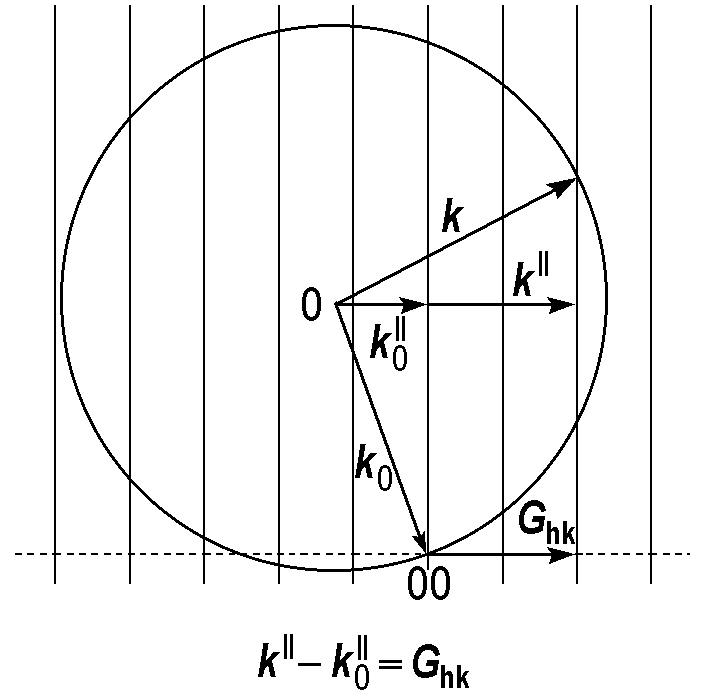
\includegraphics[width=0.4\linewidth]{evald.png}}
\caption{Построение Эвальда для дифракции на двумерной решетке 
поверхности.}
\label{pic:evald}
\end{figure}
В отличие от узлов трехмерной обратной решетки, здесь мы имеем дело 
со стержнями обратной решетки, которые проведены перпендикулярно 
поверхности через каждую точку двумерной обратной решетки.
Конец волнового вектора $\textbf{k}_0$ упирается в стержень обратной 
решетки. Пересечения стержней со сферой Эвальда определяют волновые 
векторы дифракционных пучков $\textbf{k}$.


Схема стандартной экспериментальной установки для прямого наблюдения
картин ДМЭ показана на рис.~\ref{pic:LEED_setup}(a).
	\begin{figure}[!ht]
		\center{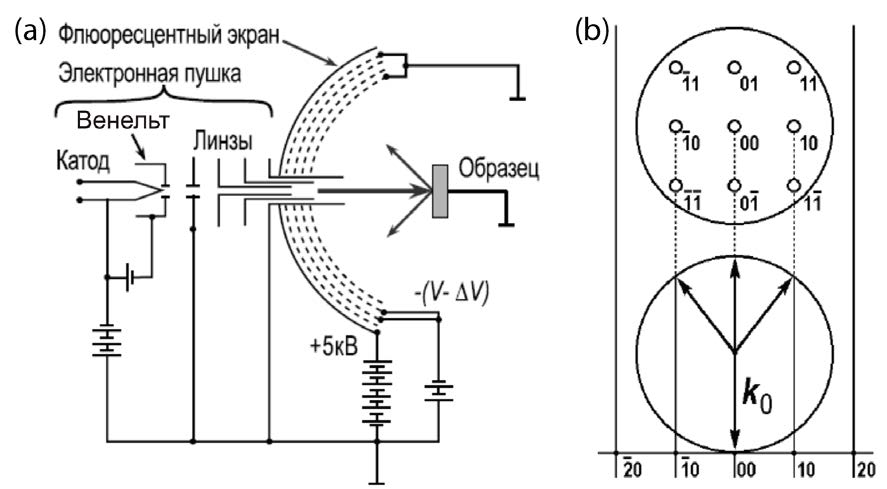
\includegraphics[width=0.7\linewidth]{leed_setup.png}}
		\caption{(a) Схема стандартной четырёх-сеточной установки для 
		наблюдения ДМЭ. (b) Обозначение дифракционных рефлексов на ДМЭ 
		картине при нормальном падении первичного пучка электронов. Рефлексы 
		имеют те же индексы, что и соответствующие узлы двумерной обратной 
		решётки.}
		\label{pic:LEED_setup}
	\end{figure}
Основные элементы установки -- это
	\vspace{15pt}
		\begin{itemize}
			\item Электронная пушка, генерирующая коллимированный пучок 
			электронов низких энергий;
			\item Держатель образца с исследуемым образцом;
			\item Полусферический флюоресцентный экран с набором из четырех 
			сеток для наблюдения картины дифракции упруго рассеянных электронов.
		\end{itemize} 
	\vspace{15pt}
Рассеянные на поверхности электроны проходят через задерживающую сетку,
отсекающую вторичные и неупруго рассеянные электроны, ускоряются и 
сталкиваются с флуоресцентным экраном, вызывая его свечение, 
детектируемое CCD-камерой.


Сравнение геометрии ДМЭ установки и построения Эвальда показывает, 
что картина дифракции, наблюдаемая на экране, соответствует обратной 
решётке поверхности. Трансляционные векторы обратной решетки 
$\textbf{b}_i$ связаны с векторами кристаллической решетки поверхности
$\textbf{a}_i$ выражениям
	\begin{equation}
		\textbf{b}_1=2\pi\frac{\textbf{a}_2\times\textbf{n}}{|\textbf{a}_1\times\textbf{a}_2|},\quad\textbf{b}_2=2\pi\frac{\textbf{n}\times\textbf{a}_1}{|\textbf{a}_1\times\textbf{a}_2|}
	\end{equation}
где \textbf{n} -- нормаль к поверхности.
Наблюдаемые рефлексы индексируются также, как и 
узлы обратной решетки, а именно величинами $h$, $k$. Зеркальный рефлекс
принято приписывать к точке $(0,0)$. При нормальном падении первичного
пучка электронов он находится в центре картины ДМЭ рис.~\ref{pic:LEED_setup}(б).


Для анализа картины ДМЭ сначала качественно оценивают структурное
совершенство изучаемой поверхности. От хорошо упорядоченной поверхности
наблюдается картина ДМЭ с яркими четкими рефлексами и низким уровнем
фона. Присутствие структурных дефектов приводит к тому, что рефлексы
становятся менее интенсивными и более размытыми, а уровень фона 
возрастает. Отсутствие каких-либо рефлексов на картине ДМЭ указывает
на то, что поверхность разупорядоченная (аморфная или мелкодисперсная
поликристаллическая).


Следующий шаг заключается в рассмотрении геометрического расположения
рефлексов. ДМЭ картина типа $1\times1$ представляет наиболее простой
случай. Очевидно, что поверхность, имеющая структуру нижележащих 
плоскостей подложки, дает именно такую картину.


Если на поверхности образуется сверхструктура, то в дифракционной 
картине появляются новые рефлексы. Эти рефлексы называют 
дополнительными, чтобы отличать их от основных рефлексов, образующих
картину $1\times1$.


Таким образом, ДМЭ позволяет быстро характеризовать качество полученных
пленок адсорбата и определять параметры обратной решетки поверхности 
из геометрии дифракционной картины.






\section{Рентгеновская фотоэлектронная спектроскопия} \label{method_XPS}

Одним из самых мощных и информативных инструментов для изучения 
энергетического спектра заполненных электронных состояний вещества
является фотоэлектронная спектроскопия. Она делится на две методики,
отличающиеся задачами исследования и энергиями фотонов:
	\vspace{15pt}
		\begin{itemize}
			\item \textit{Рентгеновская фотоэлектронная спектроскопия}(РФЭС) 
			применяется в основном для анализа остовных электронных уровней,
			поэтому используется рентгеновское излучение в диапазоне энергий
			фотонов около $100-10 000 \si{\eV}$.
			\item \textit{Ультрафиолетовая фотоэлектронная спектроскопия}(УФЭС),
			используется преимущественно для анализа состояний валентной зоны. Для нее характерны энергии фотонов $10-100 \si{\eV}$.
		\end{itemize}
	\vspace{15pt}


В настоящей работе использовалась методика рентгеновской 
фотоэлектронной спектроскопии, с помощью которой были изучены остовные
электронные уровни системы h-BN/Co(0001) при взаимодействии с 
молекулярным кислородом.

\paragraph{Фотоэффект.}
В основе фотоэлектронной спектроскопии лежит фотоэлектрический эффект.
Если электрон, первоначально находившийся в состоянии с энергией
связи $E_i$, поглощает фотон с энергией $\hbar\omega$ и покидает 
твердое тело, то такой электрон называется фотоэлектроном, а его
кинетическую энергию, с которой он покидает твердое тело, можно записать
в виде
	\begin{equation}
		E_{kin}=\hbar\omega-E_i-\phi,
	\end{equation}

где $\phi=E_{vacuum}-E_{Fermi}$ -- работа выхода материала рис.~\ref{pic:XPS_diagram}.
	\begin{figure}[!ht]
		\center{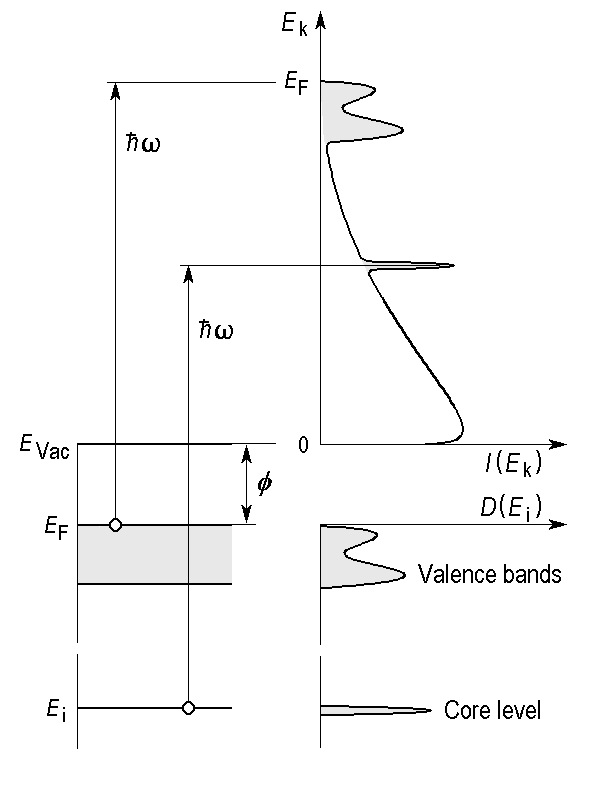
\includegraphics[width=0.5\linewidth]{xps_pic.png}}
		\caption{Схематическая диаграмма, иллюстрирующая процесс фотоэмиссии
		на поверхности металла.}
		\label{pic:XPS_diagram}
	\end{figure}


Для того, чтобы зарегистрировать фотоэлектрон, должны быть выполнены
следующие условия:
	\vspace{15pt}
		\begin{itemize}
			\item Энергия фотона должна быть достаточна, чтобы электрон смог
			покинуть твердое тело, то есть $\hbar\omega\geq E_i+\phi$.
			\item Скорость электрона должна быть направлена в сторону внешней 
			поверхности.
			\item Электрон не должен потерять энергию в столкновениях с другими
			электронами на своем пути к поверхности.
		\end{itemize}
	\vspace{15pt}


\paragraph{Трехступенчатая модель фотоэмиссии.}
Фотоэмиссию часто описывают в рамках трехступенчатой модели~\cite{Hufner2019},
где процесс фотоэмиссии разбивается на три независимые части:
	\vspace{15pt}
		\begin{enumerate}
			\item Поглощение кванта с образованием фотоэлектрона.
			\item Движение электрона к поверхности твердого тела.
			\item Выход возбужденных электронов в вакуум.
		\end{enumerate}
	\vspace{15pt}


1) На первом шаге происходит возбуждение фотоэлектронов.
Электрон поглощает фотон и, за счет полученной энергии, переходит из
невозбужденного $E_i, \textbf{k}_i$  в возбужденное состояние выше 
уровня ферми $E_f, \textbf{k}_f$. Вероятность такого перехода 
определяется золотым правилом Ферми:
	\begin{equation} 
		\label{Fermi_rule}
		w_{fi}=\frac{2\pi}{\hbar}|\left\langle\psi_f,\textbf{k}_f|H^{int}|
		\psi_i,\textbf{k}_i\right\rangle|^2\delta(E_f-E_i-\hbar\omega)
	\end{equation}
Здесь $\psi_i$ -- волновая функция, $E_i$ -- энергия начального состояния
фотоэлектрона, а  $\psi_f$ и $E_f$ -- волновая функция и энергия 
конечного состояния соответственно. Дельта функция $\delta(E_f-E_i-\hbar\omega)$
отражает закон сохранения энергии. Гамильтониан $H^{int}$ взаимодействия
электрона и электромагнитного поля может быть записан как
	\begin{equation} 
	\label{equation:hamiltonian}
		H^{int}=\frac{1}{2mc}(\textbf{A}\cdot\hat{\textbf{p}}+\hat{\textbf{p}}\cdot\textbf{A})
	\end{equation}
где $\hat{\textbf{p}}$ -- оператор импульса и $\textbf{A}$ -- векторный потенциал электромагнитного поля. Для бесспиновой частицы гамильтониан
\ref{equation:hamiltonian} может быть приведен к виду
	\begin{equation} 
		\label{equation:hamiltonian}
		H^{int}=\frac{1}{mc}(\textbf{A}\cdot\hat{\textbf{p}})
	\end{equation}
Если представить векторный потенциал \textbf{A} в виде разложения по
плоским волнам, можно показать, что матричный элемент перехода
будет пропорционален
	\begin{equation} 
		\label{equation:spinless_electron_hamiltonian}
		\left\langle\psi_f,\textbf{k}_f|H^{int}|
		\psi_i,\textbf{k}_i\right\rangle\sim
		\left\langle\psi_f,\textbf{k}_f|\textbf{ep}e^{i\textbf{k}r}|
		\psi_i,\textbf{k}_i\right\rangle
	\end{equation}
где \textbf{e} -- это вектор поляризации, а \textbf{k} -- волновой вектор
падающего излучения. В длинноволновом (дипольном) приближении $e^{i\textbf{k}r}\rightarrow 1$, 
тогда вероятность перехода становится пропорциональна
$\left\langle\psi_f,\textbf{k}_f|\textbf{ep}|\psi_i,\textbf{k}_i\right\rangle$. Также в этом приближении для гамильтониана
\ref{equation:spinless_electron_hamiltonian} можно вывести 
правила Лапорта для орбитального и спинового квантовых чисел:
$\Delta\l=\pm1,\ \Delta$$S=0$.


2) На втором шаге трехступенчатой модели фотоэмиссии возбужденный
фотоэлектрон проходит через твердое тело на поверхность. В течение 
этого перемещения, фотоэлектрон может испытывать рассеяние при 
взаимодействии с фононами или другими электронами. Упруго рассеянные
фотоэлектроны от нерассеянных различаются по времени, которое они 
тратят на достижение поверхности, и направлению волнового вектора. 
Неупруго рассеянные фотоэлектроны теряют энергию в процессе рассеяния
и достигают поверхности с куда меньшей энергией, чем упруго рассеянные.
Такие электроны называют вторично рассеянными. 
Расстояние, которое преодолевает электрон в твердом теле до первого 
рассеяния, называется длиной свободного пробега и является функцией 
энергии $\lambda(E)$. Длина свободного пробега не зависит от материала.
Кривая зависимости глубины выхода электрона от кинетической энергии для нескольких различных элементов показана на рис.~\ref{pic:mean_free_path}.
	\begin{figure}[!ht]
		\center{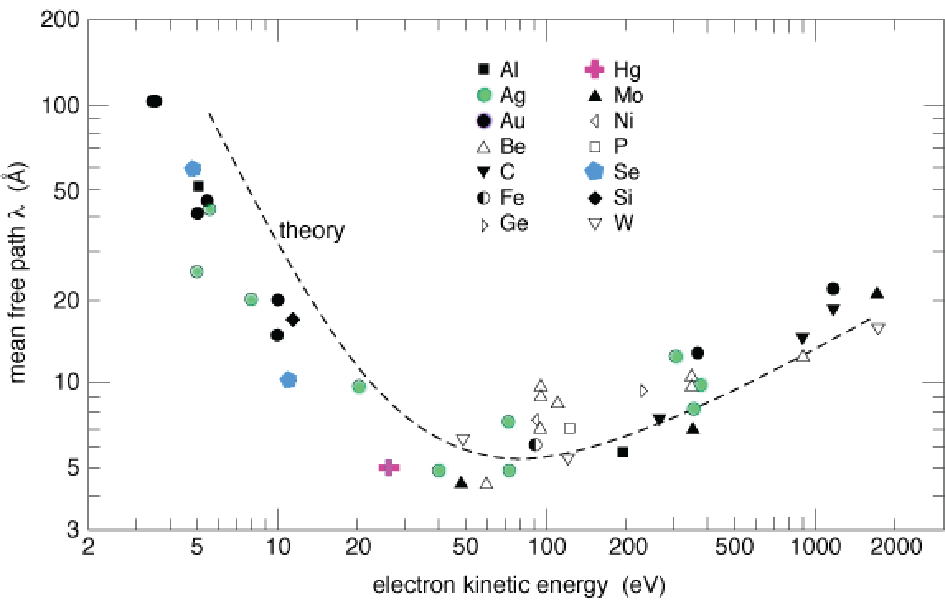
\includegraphics[width=0.7\linewidth]{mean_free_path.png}}
		\caption{Набор экспериментальных данных для длин свободного пробега 
		электронов в различных материалах, представленных в виде зависимости 
		от кинетической энергии электронов~\cite{Mean_Free_Path}.}
		\label{pic:mean_free_path}
	\end{figure}
Медленные электроны с энергией $<10\si{\eV}$ слабо 
взаимодействуют с фононами и электронами и поэтому проходят большие
дистанции. Минимум $\lambda(E)$ приходится на энергии $30-200\si{\eV}$.
На этих энергиях вероятность рассеяния электрона увеличивается, в
основном, за счет неупругого взаимодействия и возбуждения плазмонов.
Для быстрых высокоэнергетических электронов с энергией $>200\si{\eV}$
эффективное сечение рассеяния уменьшается, в результате чего $\lambda(E)$ растет.


3) На третьем шаге трехступенчатой модели фотоэмиссии электроны,
достигшие поверхности твердого тела, должны преодолеть потенциальный
барьер высотой $eV_0=E_{vac}-E_0$ между наивысшим заполненным уровнем
и уровнем вакуума~\ref{pic:final_state_photoemission}(a). 
	\begin{figure}[!ht]
		\center{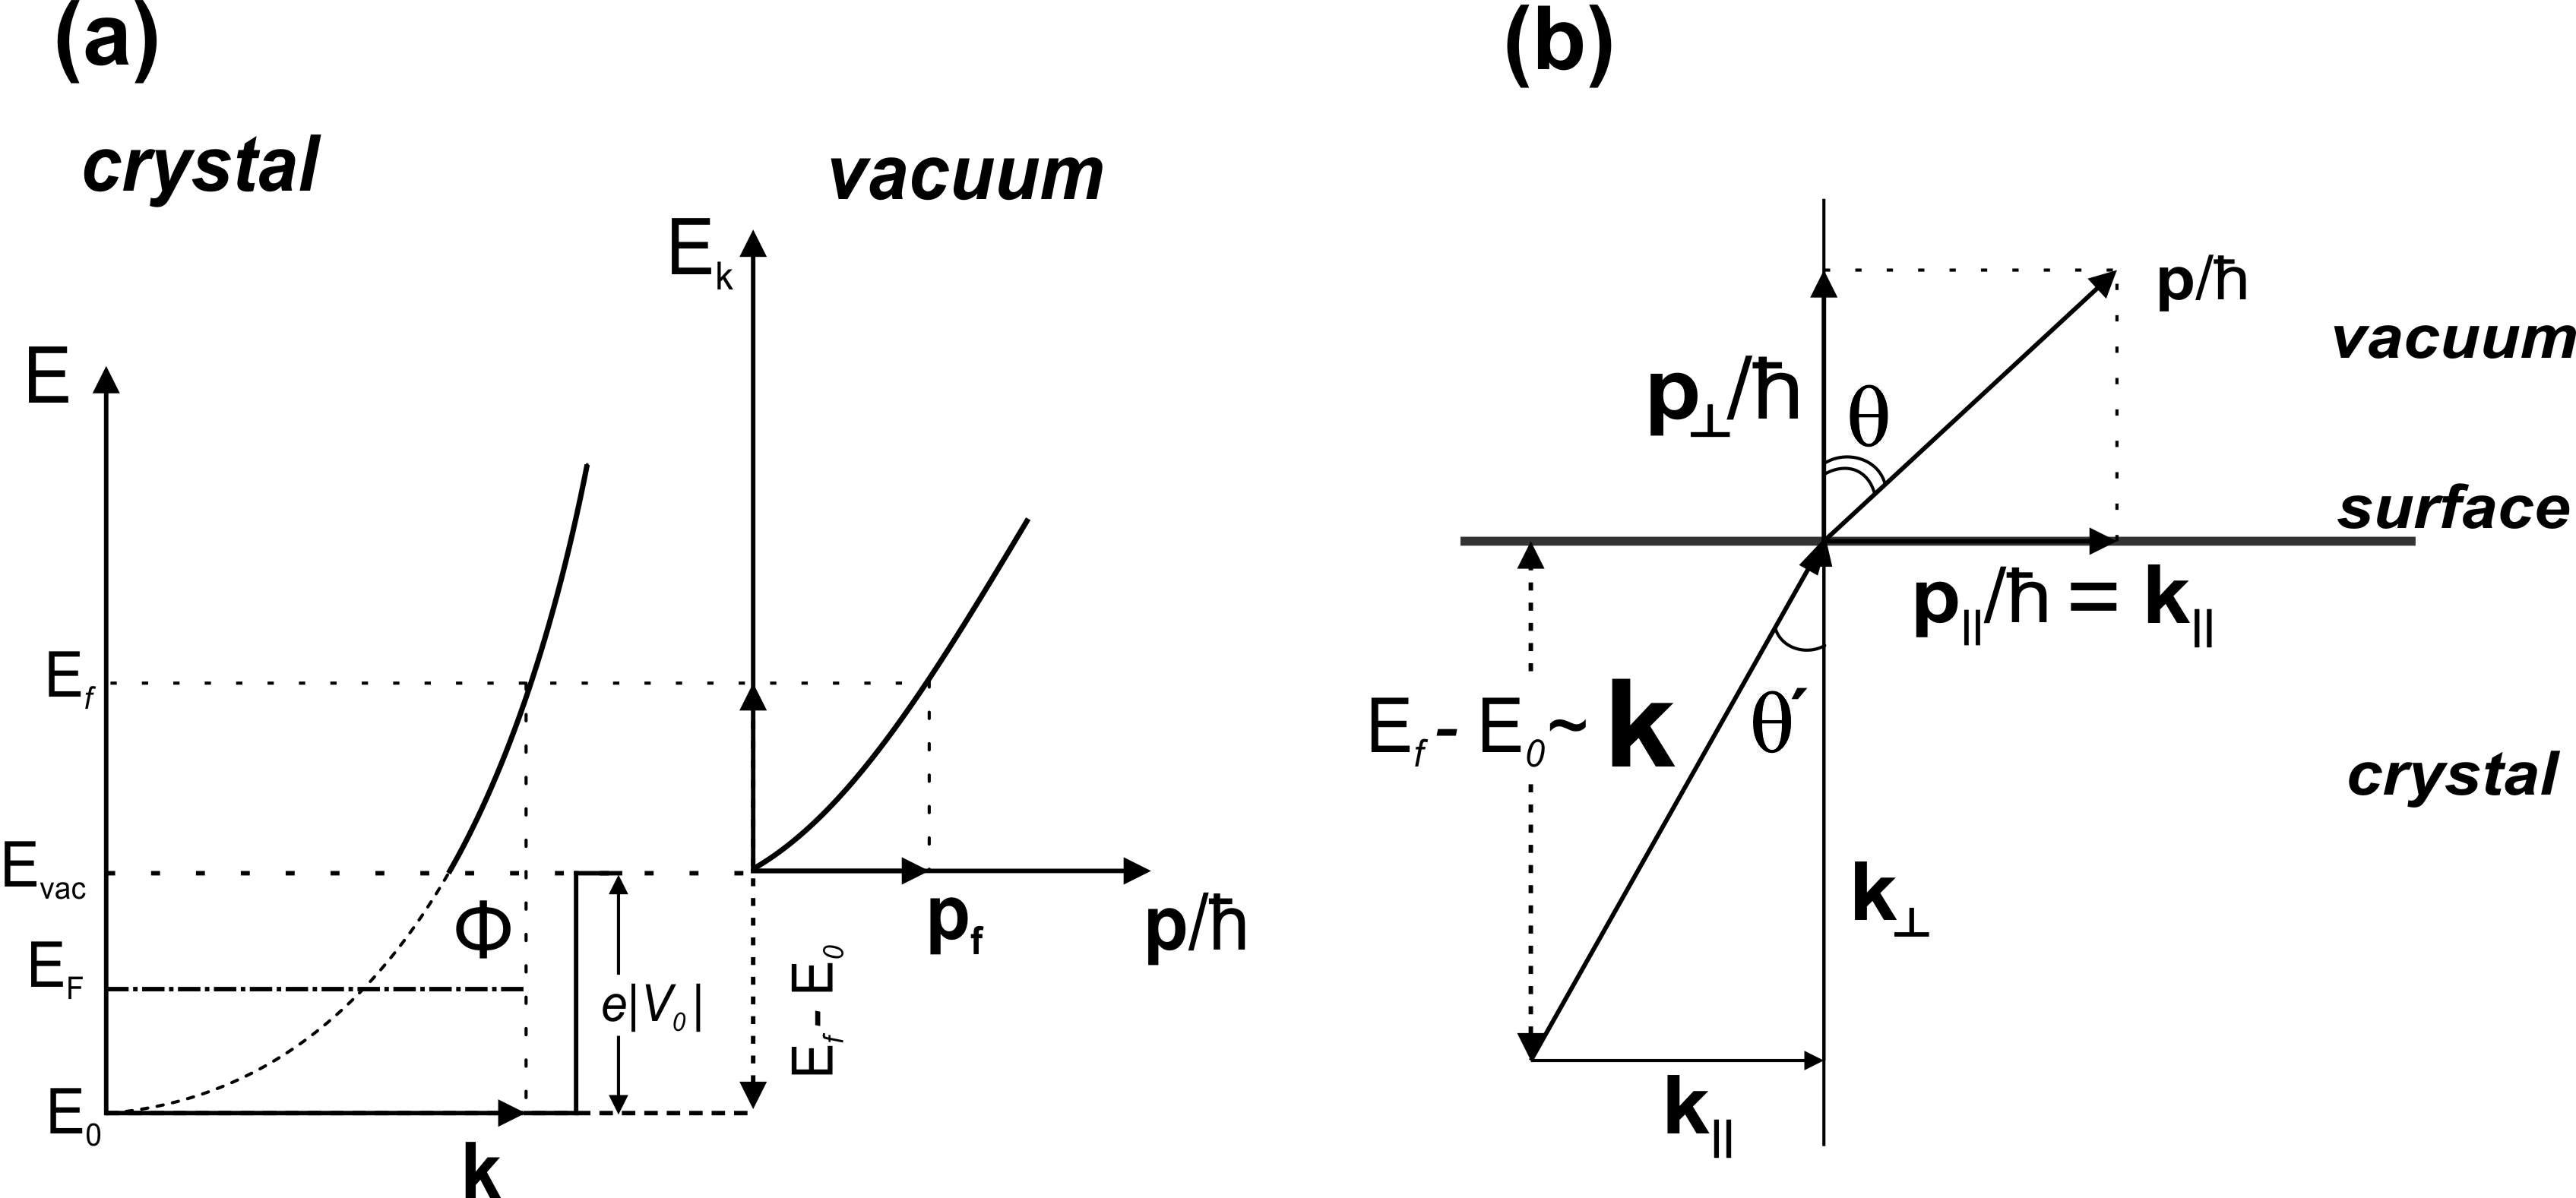
\includegraphics[width=0.7\linewidth]{final_state_photoemission.png}}
		\caption{Схематическая иллюстрация финальной стадии фотоэмиссии(a), 
		Закон Снеллиуса для фотоэлектронов(b).}
		\label{pic:final_state_photoemission}
	\end{figure}
При переходе через поверхность параллельная составляющая вектора 
электрона сохраняется (т.к. ничего не влияет на эту величину), а 
перпендикулярная составляющая уменьшается на величину, определяемую 
внутренним потенциалом кристалла (в вакууме кинетическая энергия 
отсчитывается от уровня вакуума, а в твёрдом теле -- от дна 
“потенциального ящика”, глубина которого определяется внутренним 
потенциалом). Это приводит к преломлению электронной волны на выходе 
из кристалла~\ref{pic:final_state_photoemission}(b).


\paragraph{Анализ атомного состава с помощью РФЭС.} 
РФЭС может быть использована для определения атомного состава образца.
В основе количественного анализа химического состава образца с 
помощью РФЭС лежат следующие предположения:
	\vspace{15pt}
		\begin{itemize}
			\item Поверхность образца идеально плоская;
			\item Исследуемый образец является поликристаллическим или
			аморфным, или же влияние кристаллической структуры на угловое
			распределение фотоэлектронов пренебрежимо мало;
			\item Ослабление пучка фотоэлектронов при движении в твердом теле
			имеет экспоненциальную зависимость от пройденного пути;
			\item Поверхностным отражением и преломлением можно пренебречь.
		\end{itemize}
	\vspace{15pt}
В случае пренебрежения упругим рассеянием фотоэлектронов, выражение
для интенсивности фотоэлектронной линии тонкого монослоя:
	\begin{equation}
		I=nf\frac{d\sigma_{nl}(h\nu,\gamma)}{d\Omega}AT(E_k),
	\end{equation}
где $E_k$ -- кинетическая энергия фотоэлектронов, формирующих пик, 
\textit{n} -- концентрация атомов, \textit{f} -- поток фотонов,
$\frac{d\sigma_{nl}(h\nu,\gamma)}{d\Omega}$ -- дифференциальное
сечение фотоионизации, \textit{A} -- площадь области анализа, $T(E_k)$ -- 
функция пропускания спектрометра.



Также РФЭС спектр содержит информацию о химическом состоянии атомов
составляющих поверхность. Точные измерения энергетического положения 
остовного уровня для данного элемента показывают, что положение уровня 
меняется в зависимости от химического состояния атома, которое зависит 
от типа атомов окружения и характера химического связывания с ними.
Такие смещения называют химическими сдвигами.
Химический сдвиг относительно его положения в нейтральном атоме может 
быть как положительным, так и отрицательным и изменяться в пределах
нескольких $\si{\eV}$. Объяснить природу химического сдвига 
в простейшем случае можно следующим образом:
	\vspace{15pt}
		\begin{itemize}
			\item Энергия связи электронов состоит из двух основных вкладов: 
			кулоновского притяжения к ядру и межэлектронного взаимодействия.
			\item В результате образования химической связи происходит 
			перераспределение плотности валентных электронов взаимодействующих
			атомов, следствием этого является изменение химического состояния
			атома и его энергии связи.
			\item При увеличении заряда на данном атоме происходит усиление
			электронного экранирования, в связи с чем связь электрона ослабевает.
			В противоположном случае, при уменьшении заряда, электронное
			экранирование ослабевает, и энергия связи увеличивается.
		\end{itemize}
	\vspace{15pt}
Если химсдвиг $<0.5\si{\eV}$, то оказывается невозможным
его определить "на глаз". В этом случае необходимо многокомпонентный
пик разложить на отдельные компоненты. Форма остовной линии 
представляет собой свёртку Лоренциана
	\begin{equation} 
		\label{equation: Lorenc}
		L_h(E)=\frac{1}{\pi \beta}\left(1+\left[\frac{E}{\beta}\right]^2\right)^{-1},
	\end{equation}
обусловленного конечным временем жизни возбуждённого состояния атома, 
и Гауссиана
	\begin{equation}
		G_h(E)=exp\left(-\ln{2\left[\frac{E}{\beta}\right]^2}\right),
	\end{equation}
ширина которого определяется главным образом инструментальным 
разрешением. 


Продуктом асимметрии Гауссиана и Лоренциана одинаковой ширины
и высоты является
	\begin{equation}
		GL_p(E)=\left(1+M\left[\frac{E}{\beta+\alpha E}\right]^2\right)^{-1}
		exp\left(-(1-M)\ln{2\left[\frac{E}{\beta+\alpha E}\right]^2}\right),
	\end{equation}
где $\alpha\geq0$ -- асимметрия, $M$ -- смешанное отношение от 0 
(чистый Гауссиан) до 1 (чистый Лоренциан).


Сумма асимметрии Гаусииана и Лоренциана одинаковой ширины и высоты:
	\begin{equation}
		GL_s(E)=\left(1+M\left[\frac{E}{\beta+\alpha E}\right]^2\right)^{-1}
		+(1-M)
		exp\left(-\ln{2\left[\frac{E}{\beta+\alpha E}\right]^2}\right).
	\end{equation}


В настоящей работе при разложении спектров фотоэмиссии использовались
именно эти формулы.



\section{Спектроскопия поглощения рентгеновских лучей}

Спектроскопия, основанная на изучении ближней тонкой структуры 
рент­геновских спектров поглощения (БТСРСП или NEXAFS: Near-Edge 
X-ray Absorbtion Fine Structure), позволяет изучать свободные 
состояния зоны про­водимости~\cite{Stohr1992}. В этом методе, в 
зависимости от энергии фотонов в окрестности края поглощения,
измеряется коэффициент поглощения рентгеновских лучей.
	\begin{figure}[!ht]
		\center{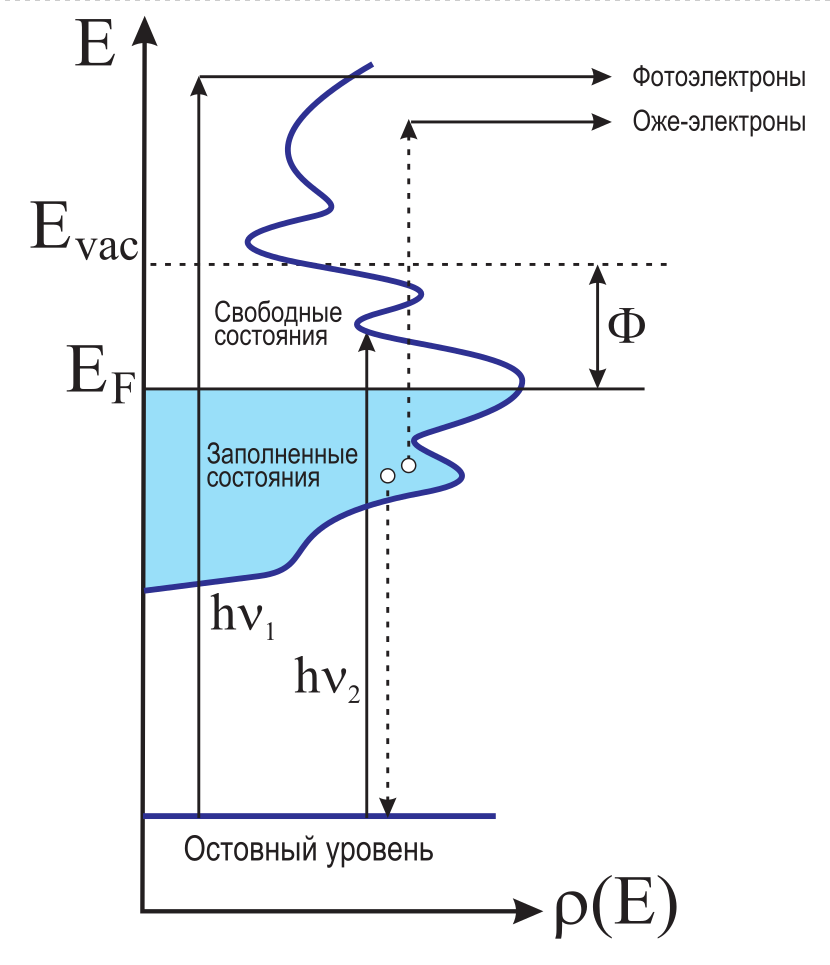
\includegraphics[width=0.5\linewidth]{NEXAFS_pic.png}}
		\caption{Спектроскопия NEXAFS: упрощенная энергетическая диаграмма.}
		\label{pic:NEXAFS_diagram}
	\end{figure}
В процессе фотовозбуж­дения электрон переходит из начального состояния \textit{i} в конечное состояние \textit{f}, как это уже упоминалось в разделе \ref{method_XPS}.
На диаграмме рис.~\ref{pic:NEXAFS_diagram} показано, что остовный уровень
соответствует начальному состоянию, а конечное стостояние лежит в зоне 
проводимости. Так как остовный уровень характеризуется фиксированным значением энергии, то появляется возможность задавать энергию конечного состояния в соот­ветствии
с законом сохранения энергии $E_f=E_i+h\nu$, при помощи выбора $h\nu$
вблизи края поглощения. 

Экспериментально спектроскопия поглощения может быть реализована разными
способами. В настоящей работе использовался метод измерения полного квантового выхода 
электронов (TEY: TolalElectron Yield) – среднего числа электронов, выбиваемых из образца одним фо­тоном. Так как выходу электронов всегда предшествует
поглощение фотонов, то 
зависимость полного выхода от энергии фотонов слабо отличается от
зависимости коэффициента поглощения. В этом случае возможна эмиссия электронов. Примеры таких процессов
показаны на рис.\ref{pic:NEXAFS_diagram}.
% Если энергии фотонов $h\nu_2$ недостаточно для прямого вы­хода
% фотоэлектрона в вакуум, то возможна эмиссия в результате Оже-процесса
% с участием электронов валентной зоны. Если же энергия фотона $h\nu_1$ достаточ­но
%  высока, то возможен как Оже процесс, так и прямой выход фотоэлектрона
% из твердого тела. Необходимо отметить, что спектроскопия полного квантово­
% го выхода, является поверхностно-чувствительным методом, но глубина анализа
% обычно больше, чем в фотоэлектронной спектроскопии, и составляет несколько
% нанометров. Причиной является то, что значительный вклад в полный выход
% дают вторичные электроны, выходящие с большей глубины, чем первичные фо­тоэлектроны.

Полный квантовый выход пропорционален интенсивности излучения, а так­же
току через образец. Поэтому для измерений используется пикоамперметр.
Источником фотонов является канал вывода СИ, обеспечивающий возможность
изменения энергии рентгеновского излучения, а также измерения потока фото­нов.


% Использование излучения с линейной поляризацией расширяет возможно­
% сти анализа многих систем с $sp^2$ гибридизацией, включая графен. В частности,
% измерение зависимости спектров NEXAFS от направления вектора поляриза­ции
% фотонов относительно поверхности графена дает возможность выделить в
% спектрах вклады, соответствующие переходам в $\pi$- или $\sigma$-состояния зоны 
% про­водимости~\cite{Stohr1992}. Так как $\pi$-орбитали направлены перпендикулярно 
% поверхно­сти, а $\sigma$ – параллельно, то соответствующие им участки спектра поглощения
% проявляют различную зависимость коэффициента поглощения от угла между
% вектором поляризации и поверхностью. При поляризации вдоль поверхности,
% переходы в $\pi$-состояния запрещены, а переходы в $\sigma$-состояния достигают
% мак­симальной вероятности.           % Глава 2
\chapter{Взаимодействие h-BN/Co(0001) с молекулярным кислородом} \label{chapt3}

Теоретические исследования показывают, что взаимодействие монослоя гексагонального 
нитрида бора с кислородом приводит к изменению электронных и магнитных
свойств материала~\cite{Ataca2010,Zhou2010}. Важным обстоятельством является то, каким именно образом кислород
вступает во взаимодействие с монослоем h-BN, а именно: встраиваются атомы кислорода в решетку 
h-BN, или интеркалируют под монослой, не образуя связей с ним, или же являются 
адатомами на поверхности монослоя. Таким образом, в данной работе был 
исследован механизм взаимодействия молекулярного кислорода с монослоем h-BN, выращенного на 
поверхности кобальта Co(0001). Посредством серии экспериментов на Российско-Германском
канале вывода СИ синхротрона BESSY II в Берлине были получены экспериментальные 
данные XPS, NEXAFS, а так же ДМЭ. Результаты и выводы по полученным данным 
представлены в данной работе.

\section{Характеристика структуры образца}

После формирования гексагонального нитрида бора на поверхности кобальта, для контроля
качества  поверхности, была получена картина дифракции медленных электронов
рис.~\ref{pic:LEED}. Постоянные решеток Co(0001) и h-BN совпадают, 
	\begin{figure}[!ht]
		\center{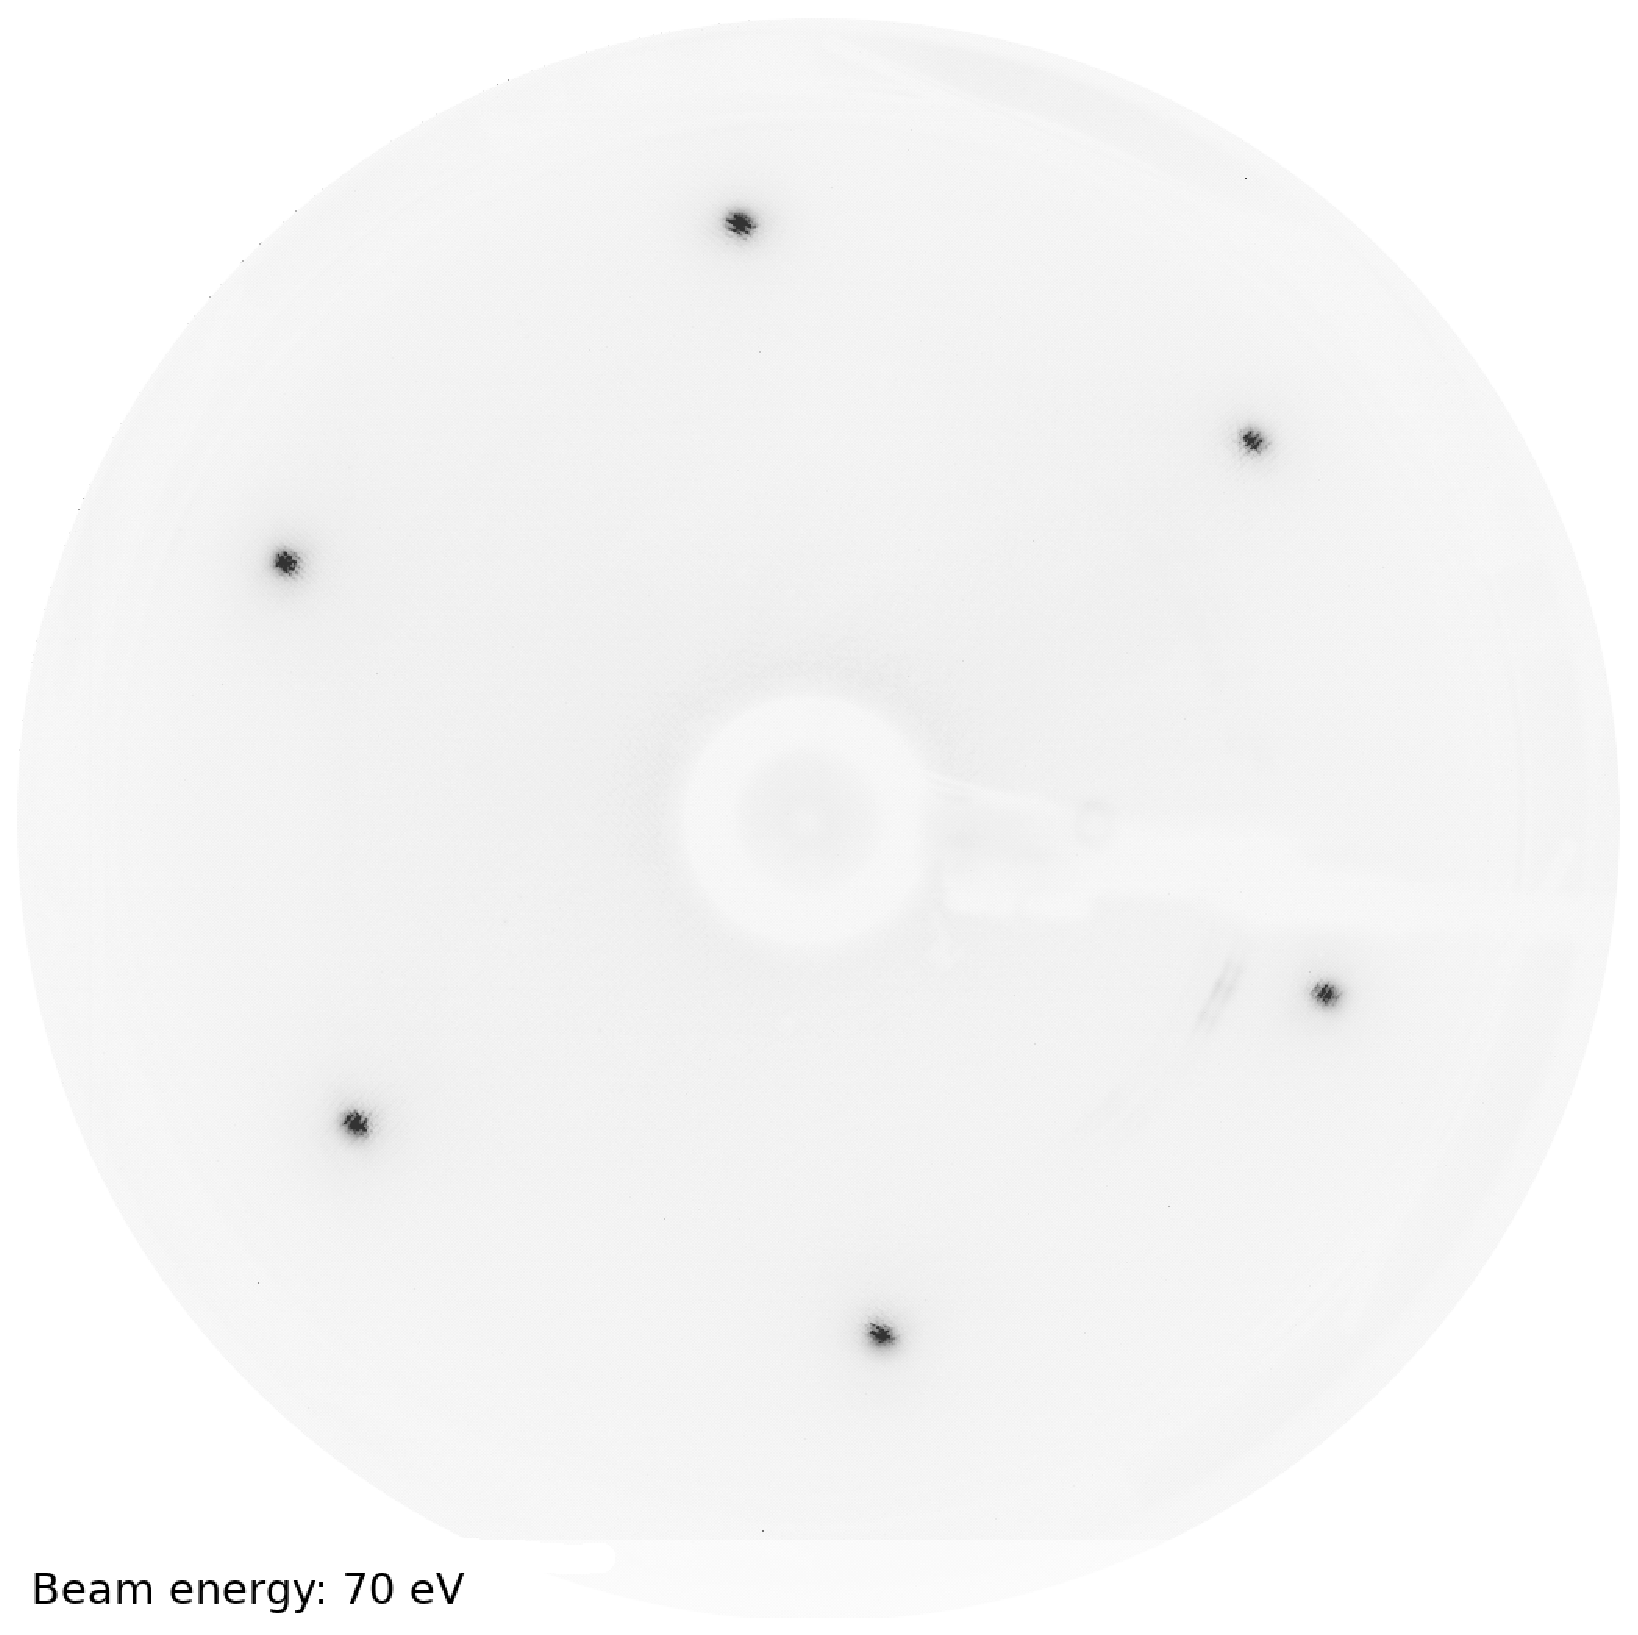
\includegraphics[width=0.3\linewidth]{LEED.eps}}
		\caption{ДМЭ картина соответствующая поверхностной фазе h-BN/Co(0001)($E_p = 70 eV$).}
		\label{pic:LEED}
	\end{figure}
этому свидетельствует четко выраженная гексагональная структура $(1\times1)$ 
и отсутствие расщепления рефлексов.
Это говорит о том, что выращенный кристалл h-BN строго
ориентирован относительно подложки.



\section{Экспериментальные спектры и их обсуждение}

Полученная система h-BN/Co(0001) прогревалась в атмосфере
кислорода. Прогрев производился поэтапно при давлении молекулярного кислорода $10^{-5}$ мбар и при температуре 300\degree C. Эти параметры выбраны 
таким образом, чтобы заметные изменения в системе происходили за времена
порядка десятков минут:
	\vspace{15pt}
		\begin{enumerate}
			\item Первый шаг. Прогрев системы h-BN/Co(0001) под давлением $10^{-5}$ мбар в течение 10 минут.
			\item Второй шаг. Прогрев системы h-BN/Co(0001) под давлением $10^{-5}$ мбар в течение 10 минут.
			\item Третий шаг. Прогрев системы h-BN/Co(0001) под давлением $10^{-5}$ мбар в течение 10 минут.
			\item Четвертый шаг. Прогрев системы h-BN/Co(0001) под давлением $10^{-5}$ мбар в течение 10 минут.
			\item Пятый шаг. Прогрев системы h-BN/Co(0001) под давлением $10^{-5}$ мбар в течение 10 минут.
			\item Шестой шаг. Прогрев системы h-BN/Co(0001) под давлением $10^{-5}$ мбар в течение 30 минут.
			\item Седьмой шаг. Прогрев системы h-BN/Co(0001) под давлением $10^{-5}$ мбар в течение 60 минут.
		\end{enumerate}
	\vspace{15pt}
Таким образом, суммарное время прогрева системы h-BN/Co(0001) в кислороде составило 140 минут.
На каждом этапе снимались РФЭС и NEXAFS спектры.
Далее в работе представленны результаты обработки и анализа полученных спектров.



\subsection{Анализ фотоэлектронных спектров}

На рис.~\ref{pic:Surveys} представлена серия фотоэлектронных спектров поверхности h-BN/Co(0001).
Каждый спектр соответствует этапу прогрева образца в кислороде. Таким образом, первый спектр характеризует
поверхность до прогрева в кислороде, а последний -- после 140 минут. Видно, что вначале
	\begin{figure}[!ht]
		\center{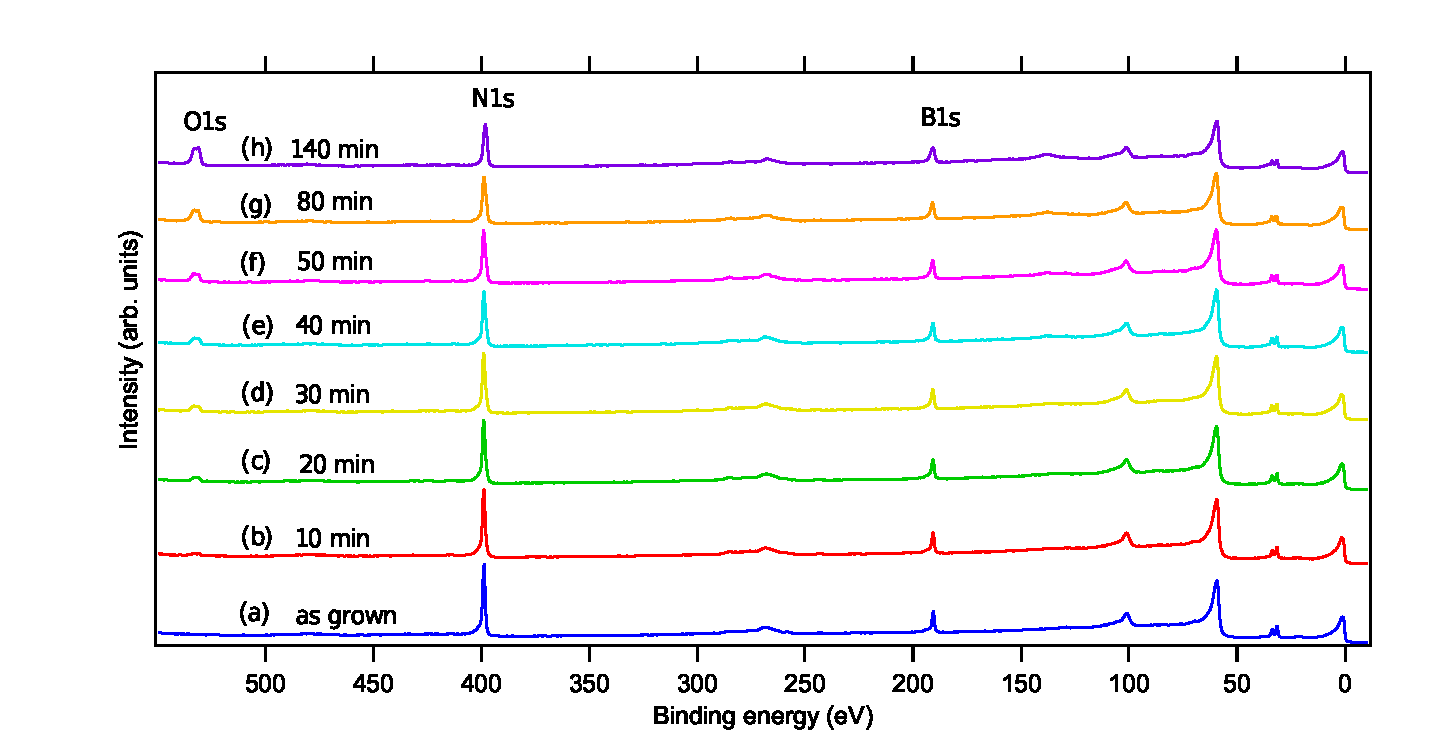
\includegraphics[width=1\linewidth]{Surveys}}
		\caption{Обзорные фотоэлектронные спектры h-BN/Co(0001) в процессе прогрева в кислороде, записанные с энергией
		возбуждающих квантов 650 eV}
		\label{pic:Surveys}
	\end{figure}
отсутствует пик кислорода O1s, который появляется уже на первом этапе после 10 минут 
прогрева h-BN/Co(0001) в кислороде, и растет со временем. Также можно заметить, что пик 
интенсивности азота N1s убывает в течение прогрева, в то время как пик 
интенсивности бора B1s остается неизменным. Зависимость концентраций азота, бора и кислорода 
в атомарных процентах на поверхности системы
h-BN/Co(0001) от времени представлена на рис.~\ref{pic:B_N_O_tot_percent}. За 100~ат\% было принято
полное количество атомов азота и бора в монослое h-BN.
На чистой поверхности образца кислород отсутствует, а на бор с азотом приходится
по 50~ат\% концентрации. Далее, с прогревом h-BN/Co(0001) в кислороде, концентрация кислорода увеличивается
и доходит до отметки в 14.9~ат\%. В процессе экспозиции концентрация азота уменьшается на 8.5~ат\%.
Концентрация бора остается постоянной. Представленные зависимости демонстрируют, что количество 
азота в кристаллической решетке гексагонального нитрида бора убывает, а кислорода возрастает.
Такое же поведение системы h-BN/Ir(111) при окислении наблюдалось в работе~\cite{Simonov2012_h-BN/Ir_Oxydation}. 
	\begin{figure}[!ht]
		\center{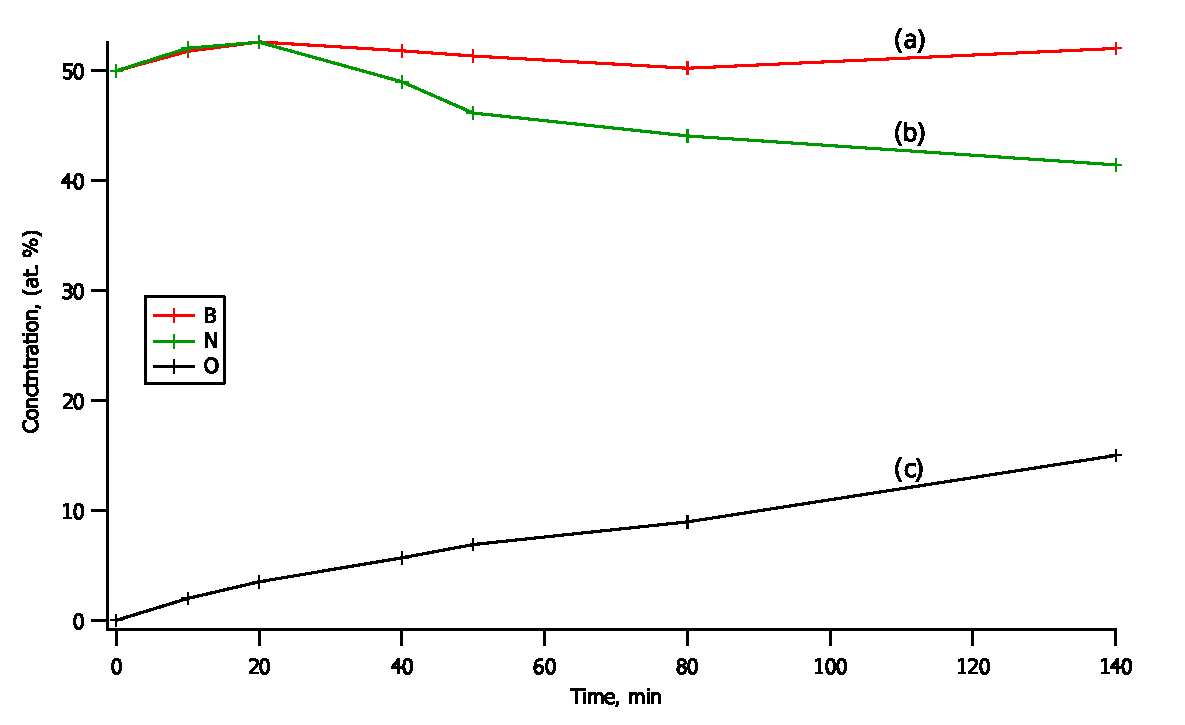
\includegraphics[width=0.8\linewidth]{N_B_O_tot_percent_vs_time}}
		\caption{Зависимость концентраций от времени (a) бора, (b) азота, (c) кислорода.}
		\label{pic:B_N_O_tot_percent}
	\end{figure}
Здесь можно сделать предположение, что атомы кислорода встраиваются в кристаллическую решетку
нитрида бора, замещая атомы азота.


Далее мы рассмотрели пики интенсивностей B1s, N1s и O1s по отдельности и пронаблюдали их эволюцию
от первого этапа с чистой поверхностью до последнего этапа после 140 минут экспозиции системы h-BN/Co(0001) в кислороде. 
На рис.~\ref{pic:B1s_N1s} представлены пики интенсивностей фотоэмиссии B1s и N1s.
	\begin{figure}[!ht]
		\center{\includegraphics[width=0.8\linewidth]{B1s_N1s_fits.eps}}
		\caption{РФЭС линии (i) B1s-, (ii) N1s-уровней от исходного h-BN (as grown) и на разных стадиях окисления.}
		\label{pic:B1s_N1s}
	\end{figure}
Пик $\mathrm{b_1}$ на рисунке~\ref{pic:B1s_N1s}(i) с энергией связи 190.4 eV соответствует основному пику 
чистого h-BN сильно связанного с Co(0001)~\cite{Usachov2018_h-BN/_PED_STM}. Уже после 10 минут прогрева системы в кислороде появляется два пика
$\mathrm{b_2}$ с энергией связи 191.3 eV и $\mathrm{b_3}$ с энергией связи 190.2 eV. Пик $\mathrm{b_3}$  имеет меньшую энергию связи. Такое появление пика интенсивности в области более низкой энергии связи может быть
связано с интеркаляцией кислорода под монослой h-BN, так, например, в работе~\cite{Usachov2017_Graphen_RS}
интеркаляция кислорода под монослой графена в системе graphen/Co(0001) тоже сопровождалась химическим сдвигом пика C1s. Пик $\mathrm{b_2}$, 
относительно $\mathrm{b_1}$, сдвинут в область больших энергий связи. Химический сдвиг в область увеличения энергии связи может быть обусловлен
образованием связи $\mathrm{B-O}$~\cite{Petravic2010}. Пик $\mathrm{b_2}$ появляется в результате встраивания кислорода
в решетку гексагонального нитрида бора с замещением атома азота на атом кислорода и образованием локальной структуры 
$\mathrm{BN_2O}$~\cite{Makarova2019_h-BN/Ni_Oxydation}.
Компонента $\mathrm{b_4}$ появляется только после 40 минут экспозиции и может
быть связана с образованием $\mathrm{BO_3}$, где уже все три атома азота замещены атомами кислорода. После 140 минут прогревания системы 
h-BN/Co(0001) пик $\mathrm{b_1}$ теряет свою интенсивность, а пики $\mathrm{b_2}$ и $\mathrm{b_3}$ становятся преобладающими. Это говорит 
нам о том, что на поверхности h-BN преимущественно образуются оксидные группы $\mathrm{BN_2O}$.
	\begin{figure}[!ht]
		\center{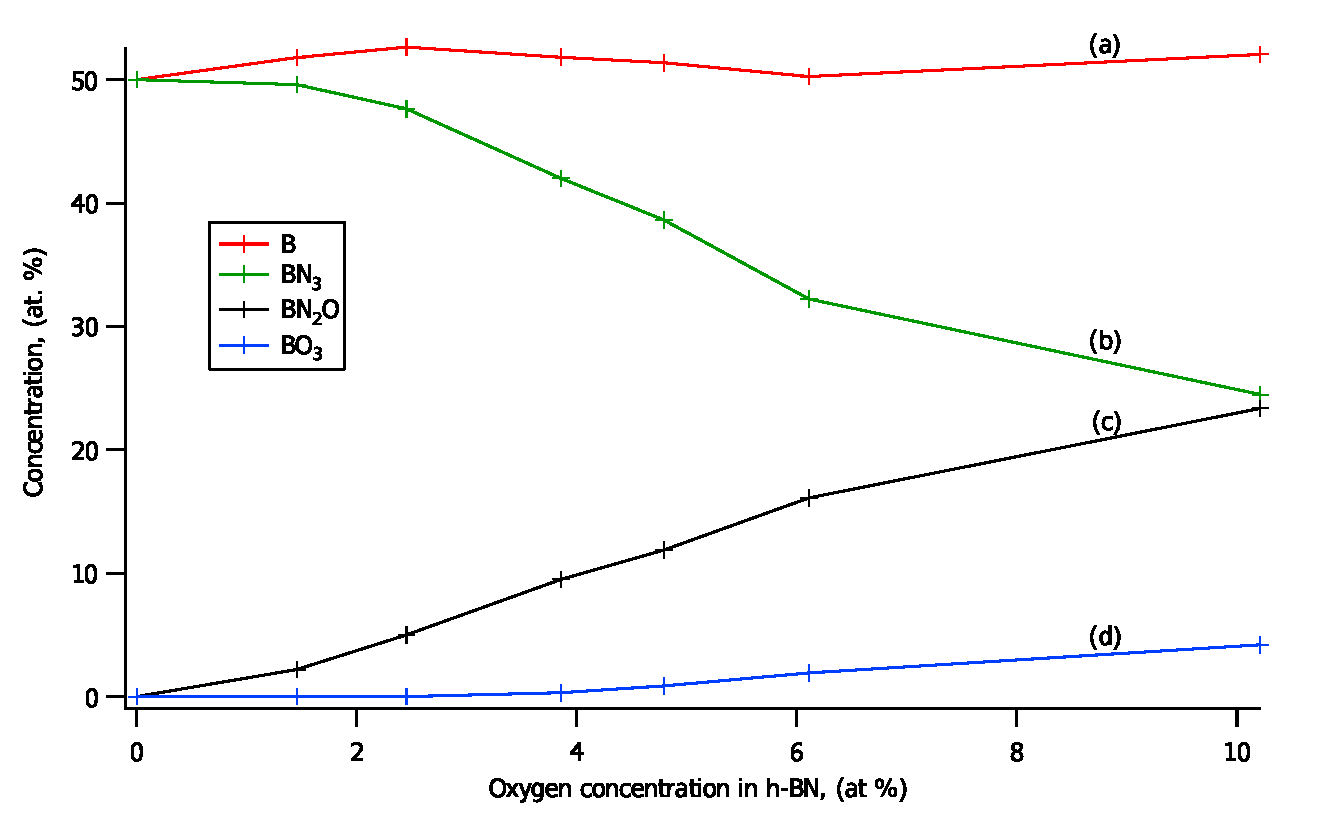
\includegraphics[width=0.8\linewidth]{Concentration_B_BN3_BN2O_BO3_vs_O.eps}}
		\caption{График зависимости концентраций B (a), $\mathrm{BN_3}$ (b), $\mathrm{BN_2O}$ (c) и $\mathrm{BO_3}$ (d) от концентрации молекулярного кислорода, встроенного в решетку гексагонального нитрида бора.}
		\label{pic:B_BN3_BN2O_BO3_vs_O}
	\end{figure}


На рис.~\ref{pic:B_BN3_BN2O_BO3_vs_O} представлен график зависимости концентраций всего бора B (a), бора, связанного с Co(0001)
$\mathrm{BN_3}$ (b), бора, связанного с одним атомом кислорода $\mathrm{BN_2O}$ (c), и бора, связанного с тремя атомами кислорода
$\mathrm{BO_3}$ (d), от концентрации кислорода, встроенного в решетку гексагонального нитрида бора. Концентрация бора (a) на поверхности
остается неизменна на протяжении всего времени экспозиции. Концентрация бора, сильно связанного с подложкой кобальта (b), характерно 
уменьшается и к седьмому этапу экспозиции с 50~ат\% убывает до 24,5~ат\%. Концентрация структуры $\mathrm{BN_2O}$, появляющейся уже после
первого этапа прогревания системы h-BN/Co(0001), растет в течение всего эксперимента и к последнему этапу возрастает до 23.3~ат\%. 
Структура $\mathrm{BO_3}$ появляется только после 40 минут экспозиции, а ее концентрация на последнем этапе доходит до отметки 4.1~атомовт\%. Таким образом, можно
сделать вывод, что с увеличением концентрации атомов кислорода в решетке h-BN, преимущественно образуются структуры вида
$\mathrm{BN_2O}$, при этом атомы бора не покидают системы h-BN/Co(0001).


На рис.~\ref{pic:B1s_N1s}(ii) представлена серия фотоэмиссионных спектров азота N1s, полученных на различных этапах прогрева h-BN/Co(0001) в кислороде.
Пик $\mathrm{n_1}$ с энергией связи 398.5 eV соответствует основному пику чистого h-BN сильно связанного с Co(0001).После 10 минут экспозиции в пике азота появляются две новые компоненты $\mathrm{n_2}$ с энергией связи 397.7 eV и $\mathrm{n_3}$ с энергией связи 397.2 eV. Энергия связи этих двух пиков меньше, чем у пика $\mathrm{n_1}$. Как было отмечено выше, такой химический сдвиг может быть результатом интеркаляции атомов кислорода под монослой h-BN. Наличие двух пиков с разным химическим сдвигом в сторону меньших энергий связи можно объяснить разным количеством  атомов кислорода под атомами азота. Общая интенсивность пика N1s в течение экспозиции уменьшается, что является следствием уменьшения количества азота в структуре h-BN/Co(0001). Другими словами, происходит десорбция атомов азота, замещенных атомами кислорода.
	\begin{figure}[!ht]
		\center{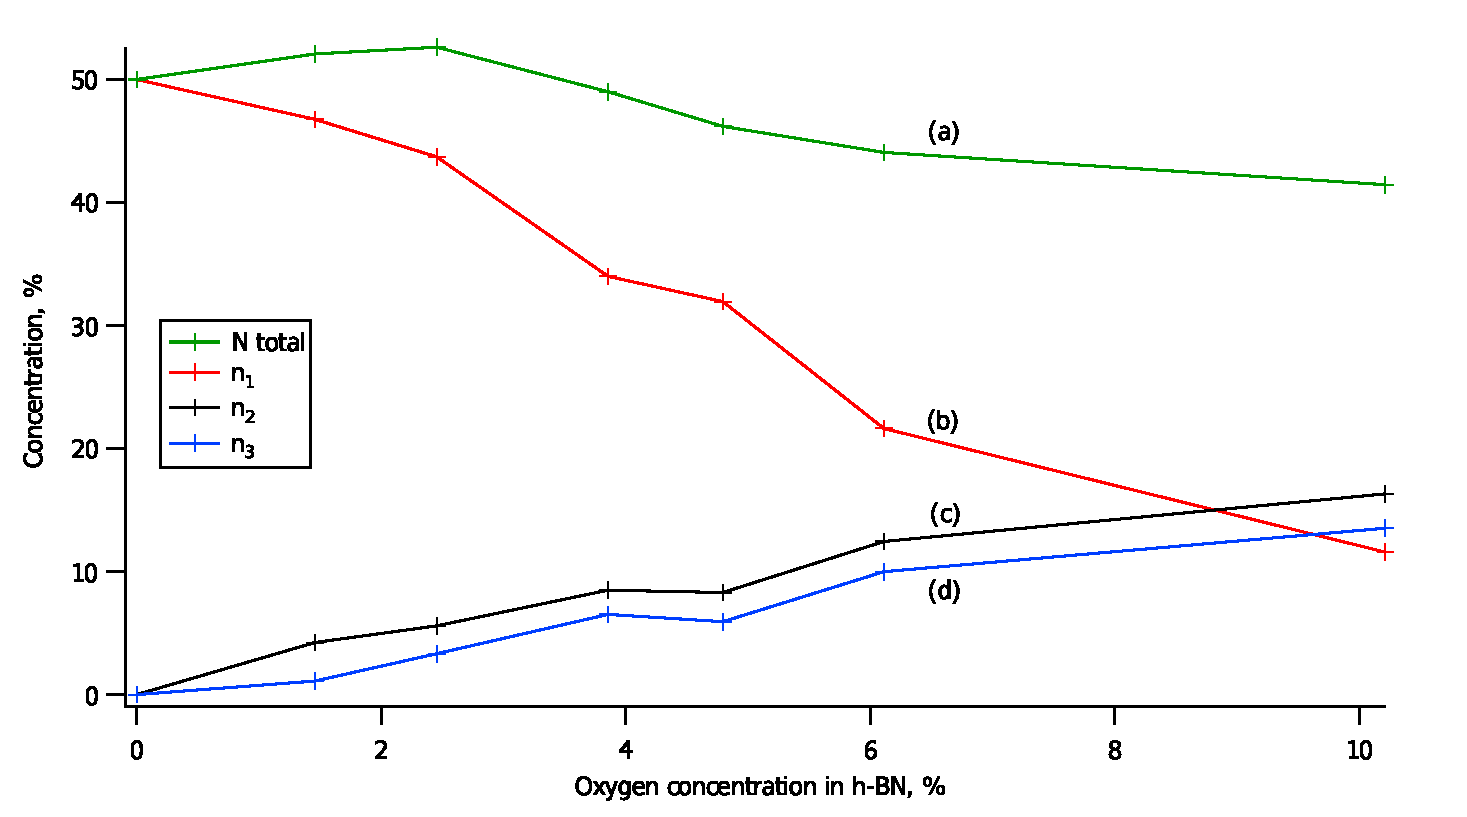
\includegraphics[width=0.8\linewidth]{Conc_Nfree_Nco_Ntot_vs_O.eps}}
		\caption{График зависимости концентраций всего азота (a), азота связанного с Co(0001) (b) и азота несвязанного с подложкой (c) и (d) от концентрации кислорода, встроенного в решетку h-BN.}
		\label{pic:Nfree_Nco_Ntot_vs_O}
	\end{figure}


Зависимость концентраций пиков азота от концентрации кислорода, встроенного в решетку гексагонального нитрида бора
представлена на рис.~\ref{pic:Nfree_Nco_Ntot_vs_O}. Кривая (a) соответствует концентрации азота на поверхности
h-BN/Co(0001). Убывание этой кривой свидетельствует о том, что, с увеличением количества атомов кислорода в решетке монослоя h-BN,
количество атомов азота уменьшается. Азоту, сильно связанному с Co(0001), соответствует 
кривая (b). Она характерно убывает с ростом концентрации кислорода, в то время как кривые (c) и (d) растут. Кривые (c) и (d) отвечают азоту, слабо связанному с подложкой кобальта в результате интеркаляции кислорода. Такое поведение 
кривых концентраций говорит о том что, вместе с процессом встраивания кислорода в решетку h-BN, так же происходит интеркаляция атомов кислорода под монослой гексагонального нитрида бора.
	\begin{figure}[!ht]
		\center{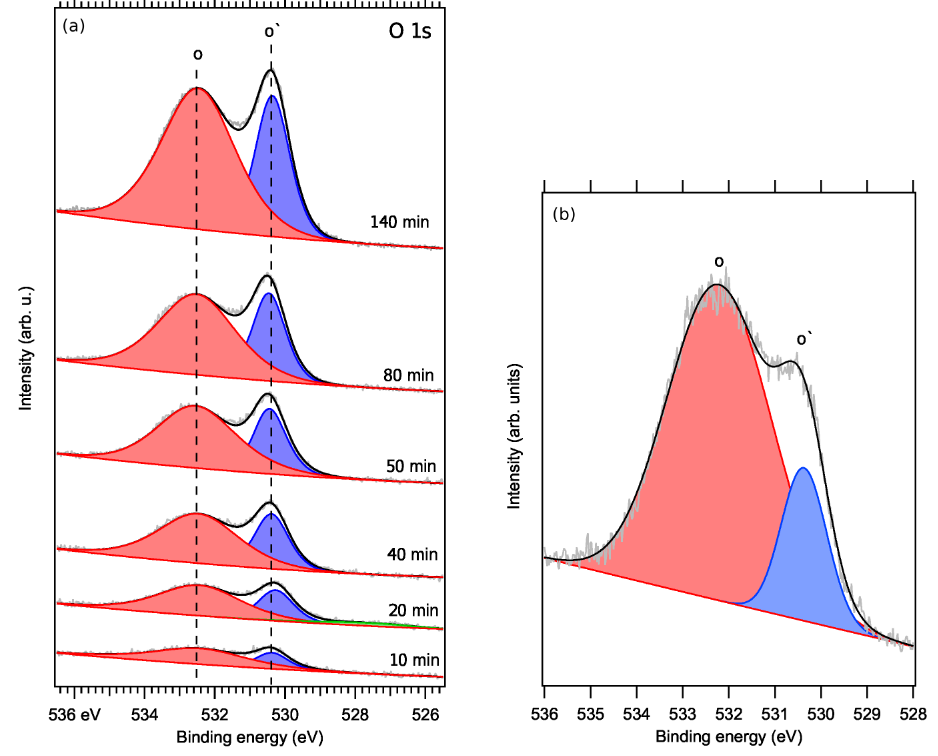
\includegraphics[width=0.7\linewidth]{O1s_all_fits_and_angle55.png}}
		\caption{РФЭС спектры O1s-уровня на разных стадиях экспозиции (a), записанный по нормали к поверхности и пик интенсивности кислорода, записанный при положении анализатора под углом 55\degree к нормали поверхности(b).}
		\label{pic:O1s_all}
	\end{figure}
На рис.~\ref{pic:O1s_all}(a) представлена серия спектров фотоэмиссии кислорода O1s в течение прогрева системы 
h-BN/Co(0001), записанная при положении анализатора по нормали к поверхности. Пик O1s содержит две компоненты: o с энергией связи 532.2 eV и o' с энергией связи 530.3 eV. Оба пика появляются после 10 минут экспозиции и растут в течение всех этапов прогрева образца в кислороде. На рис.~\ref{pic:O1s_all}(b) представлен пик интенсивности кислорода, записанный при положении анализатора под углом 55\degree к нормали поверхности. При скользящем угле выхода фотоэлектронов пик интенсивности o' рис.~\ref{pic:O1s_all}(b) почти в 5 раз меньше пика o, в то время как при выходе фотоэлектронов по нормали к поверхности рис.~\ref{pic:O1s_all}(a), этот пик меньше пика o только в 2 раза. Отсюда можно сделать вывод, что атомы кислорода находятся на разной глубине относительно поверхности системы h-BN/Co(0001), а именно, компонента o относится к атомам кислорода, которые встроились в решетку h-BN, а компонента o' характеризует атомы кислорода, интеркалировавшие под монослой гексагонального нитрида бора. Большая ширина пика o является следствием суперпозиции двух пиков оксидов $\mathrm{BN_2O}$ и $\mathrm{BO_3}$~\cite{Shevelev2019_h-BN/Co_oxydation}. 




\subsection{Анализ спектров поглощения}

Теперь рассмотрим спектры поглощения. После каждого этапа прогрева системы h-BN/Co(0001) вместе с фотоэмиссионными спектрами также снимались спектры NEXAFS. На рис.~\ref{pic:NEXAFS_B_K_edge} представлены B спектры  K-края
	\begin{figure}[!ht]
		\center{\includegraphics[width=0.8\linewidth]{BN_B_K_edge_all_40deg_to_beam.eps}}
		\caption{Спектры поглощения К-края бора.}
		\label{pic:NEXAFS_B_K_edge}
	\end{figure}
поглощения h-BN, соответствующие исходному h-BN/Co(0001) (a), через 10 минут после экспозиции с кислородом (b), 
20 минут (c), 30 минут (d), 40 минут (e), 60 минут (d) и насыщенный кислородом h-BN/Co(0001) после 240 минут экспозиции (f). Пик А соответствует гибридизированным состояниям h-BN-Co. В процессе прогрева интенсивность этого пика заметно понижается, и, после 240 минут прогрева системы, пик А становится практически незаметным. Пик B отвечает за квазисвободный гексагональный нитрид бора~\cite{Huber2015_Oxy_Stab_defffects_in_hBN}. Этот пик становится более острым в процессе прогрева h-BN/Co(0001) в кислороде, что соответствует квазисвободному h-BN и подтверждает интеркаляцию кислорода под монослой нитрида бора~\cite{Makarova2019_h-BN/Ni_Oxydation, Shevelev2019_h-BN/Co_oxydation}. Также следует
обратить внимание на пики $\mathrm{a_1}$, $\mathrm{a_2}$ и $\mathrm{a_3}$ с энергиями связи 192.7 eV, 193.3 eV и 193.9 eV соответственно. В работе \cite{Huber2015_Oxy_Stab_defffects_in_hBN} было показано, что пик $\mathrm{a_1}$ соответствует $\mathrm{BN_2O}$, пик $\mathrm{a_2}$ соответствует $\mathrm{BNO_2}$, а пик $\mathrm{a_3}$ соответствует $\mathrm{BO_3}$. Исходя из интенсивностей пиков $\mathrm{a_1}$, $\mathrm{a_2}$ и $\mathrm{a_3}$ полученного спектра поглощения B K- уровня, можно заключить, что на поверхности гексагонального нитрида бора при прогреве в кислороде преобладает образование структуры $\mathrm{BN_2O}$ в течение всего процесса прогрева. После 240 минут экспозиции также становится явно выраженным пик $\mathrm{a_3}$, что говорит о появлении структуры $\mathrm{BO_3}$ на поверхности 
h-BN/Co(0001). Пик $\mathrm{a_2}$ становится заметным только после 240 минут прогрева. Интенсивность этого пика очень низкая, а значит структуры $\mathrm{BNO_2}$ практически не образуются на поверхности гексагонального нитрида бора при прогреве системы h-BN/Co(0001) в молекулярном кислороде.



\section{Моделирование окисленного нитрида бора}

\subsection{Статистический расчет встраивания атомов кислорода в монослой h-BN}

Для лучшего понимания процесса окисления гексагонального нитрида бора было выполнено моделирование окисленной системы 
h-BN исходя из предположения, что атомы кислорода встраиваются в решетку случайным образом. В процессе моделирования
был построен фрагмент решетки гексагонального нитрида бора 200х200, который содержал 80000 атомов. Атомы азота случайным образом 
заменялись атомами кислорода. Количество атомов кислорода определялось из концентрации кислорода на поверхности в эксперименте. 
Далее были подсчитаны концентрации азота и структур вида $\mathrm{BN_3}$, $\mathrm{BN_2O}$, $\mathrm{BNO_2}$ и $\mathrm{BO_3}$ в 
кристаллической решетке  h-BN.
	\begin{figure}[!ht]
		\center{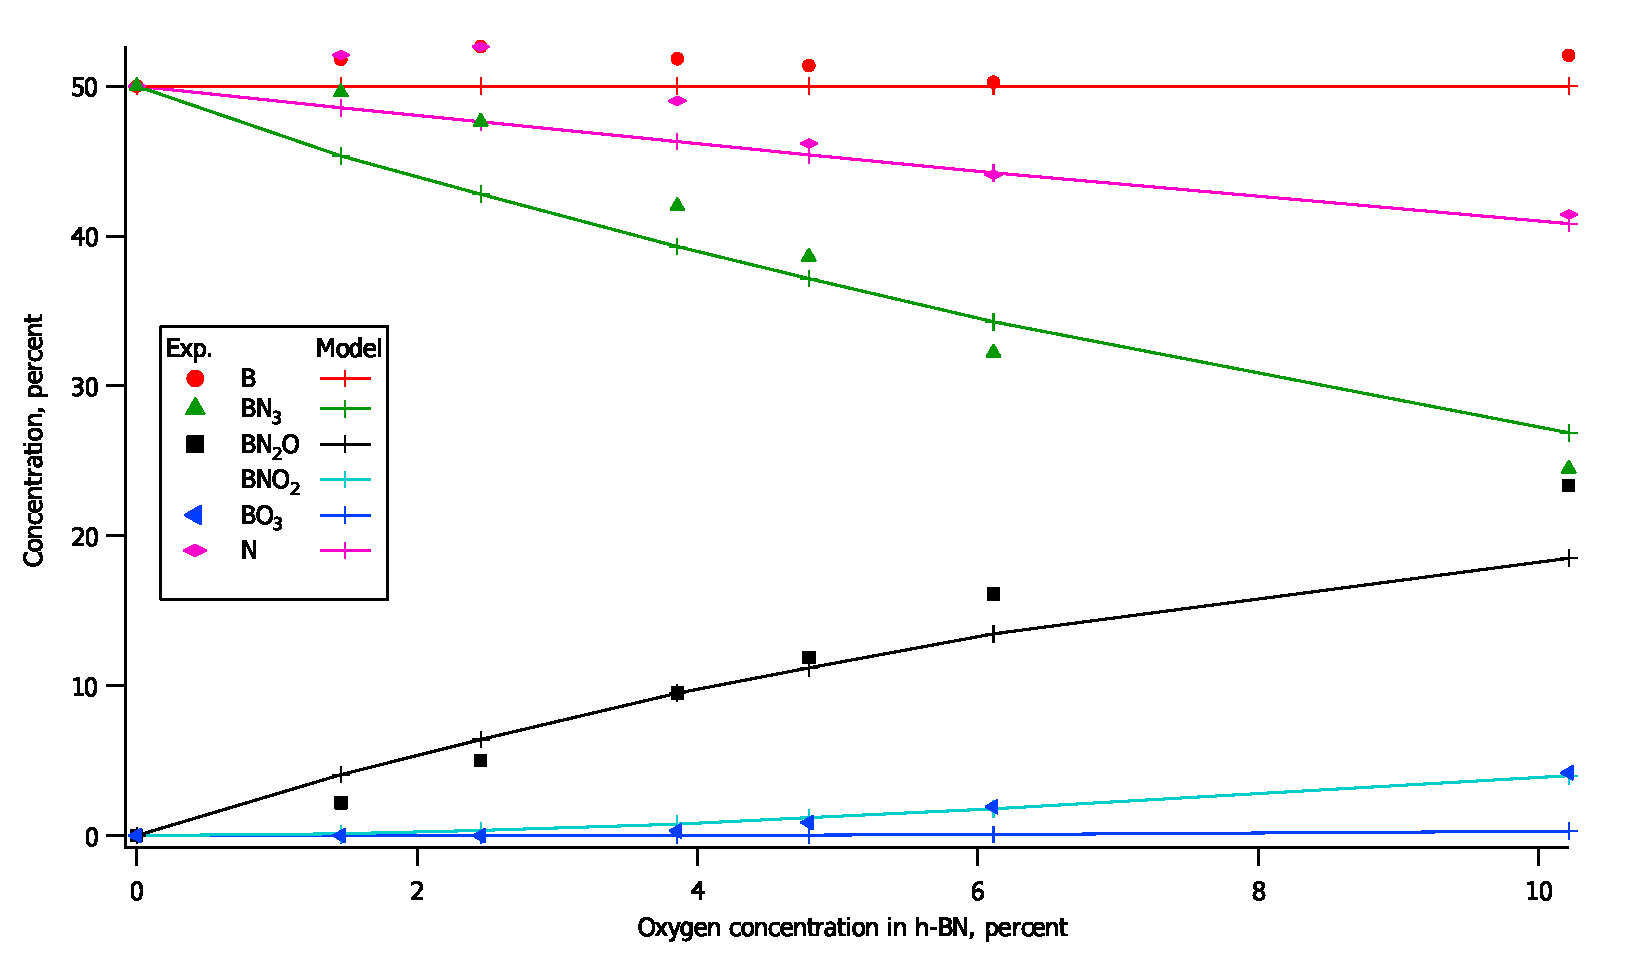
\includegraphics[width=0.8\linewidth]{BN_200x200_experiment_and_model.eps}}
		\caption{Экспериментальные и статистически рассчитанные концентрации азота и бора в зависимости от концентрации кислорода 
		в решетке h-BN.}
		\label{pic:BN_200x200_experiment_and_model}
		\end{figure}
На рис.~\ref{pic:BN_200x200_experiment_and_model} представлены для сравнения экспериментальные и статистически 
рассчитанные концентрации азота и бора в зависимости от концентрации кислорода в решетке h-BN. Из графика видно,
что все модельные кривые концентраций, кроме $\mathrm{BNO_2}$ и $\mathrm{BO_3}$, согласуются с экспериментально полученными 
концентрациями. Из расчета получается, что количество структур  $\mathrm{BNO_2}$, образующихся в результате случайного замещения,
преобладает над структурами $\mathrm{BO_3}$, что отражено на рис.~\ref{pic:BN_200x200_experiment_and_model}. Однако
в эксперименте, как было сказано ранее, структуры вида $\mathrm{BNO_2}$ практически не образовывались на поверхности.
На графике видно, что экспериментальная кривая $\mathrm{BO_3}$ совпадает с модельной кривой $\mathrm{BNO_2}$. Отсюда
можно сделать вывод, что в реальном эксперименте структуры $\mathrm{BNO_2}$ практически не образуются, вместо них
сразу появляются структуры $\mathrm{BO_3}$. 


\subsection{Расчет структуры \textbf{$\mathrm{BNO_2}$}}

Чтобы понять почему структуры вида $\mathrm{BNO_2}$ не образуются в эксперименте, с помощью  теории функционала плотности (DFT) в программе
FPLO(full-potential local-orbital minimum-basis code)~\cite{Koepernik1999} была рассчитана такая структура. Для этого рассмотрена ячейка гексагонального 
нитрида бора в вакууме. Элементарная ячейка содержала встроенные атомы кислорода таким образом, что они образовывали структуру $\mathrm{BNO_2}$. 
\begin{figure}[!ht]
\begin{minipage}[h]{0.49\linewidth}
\center{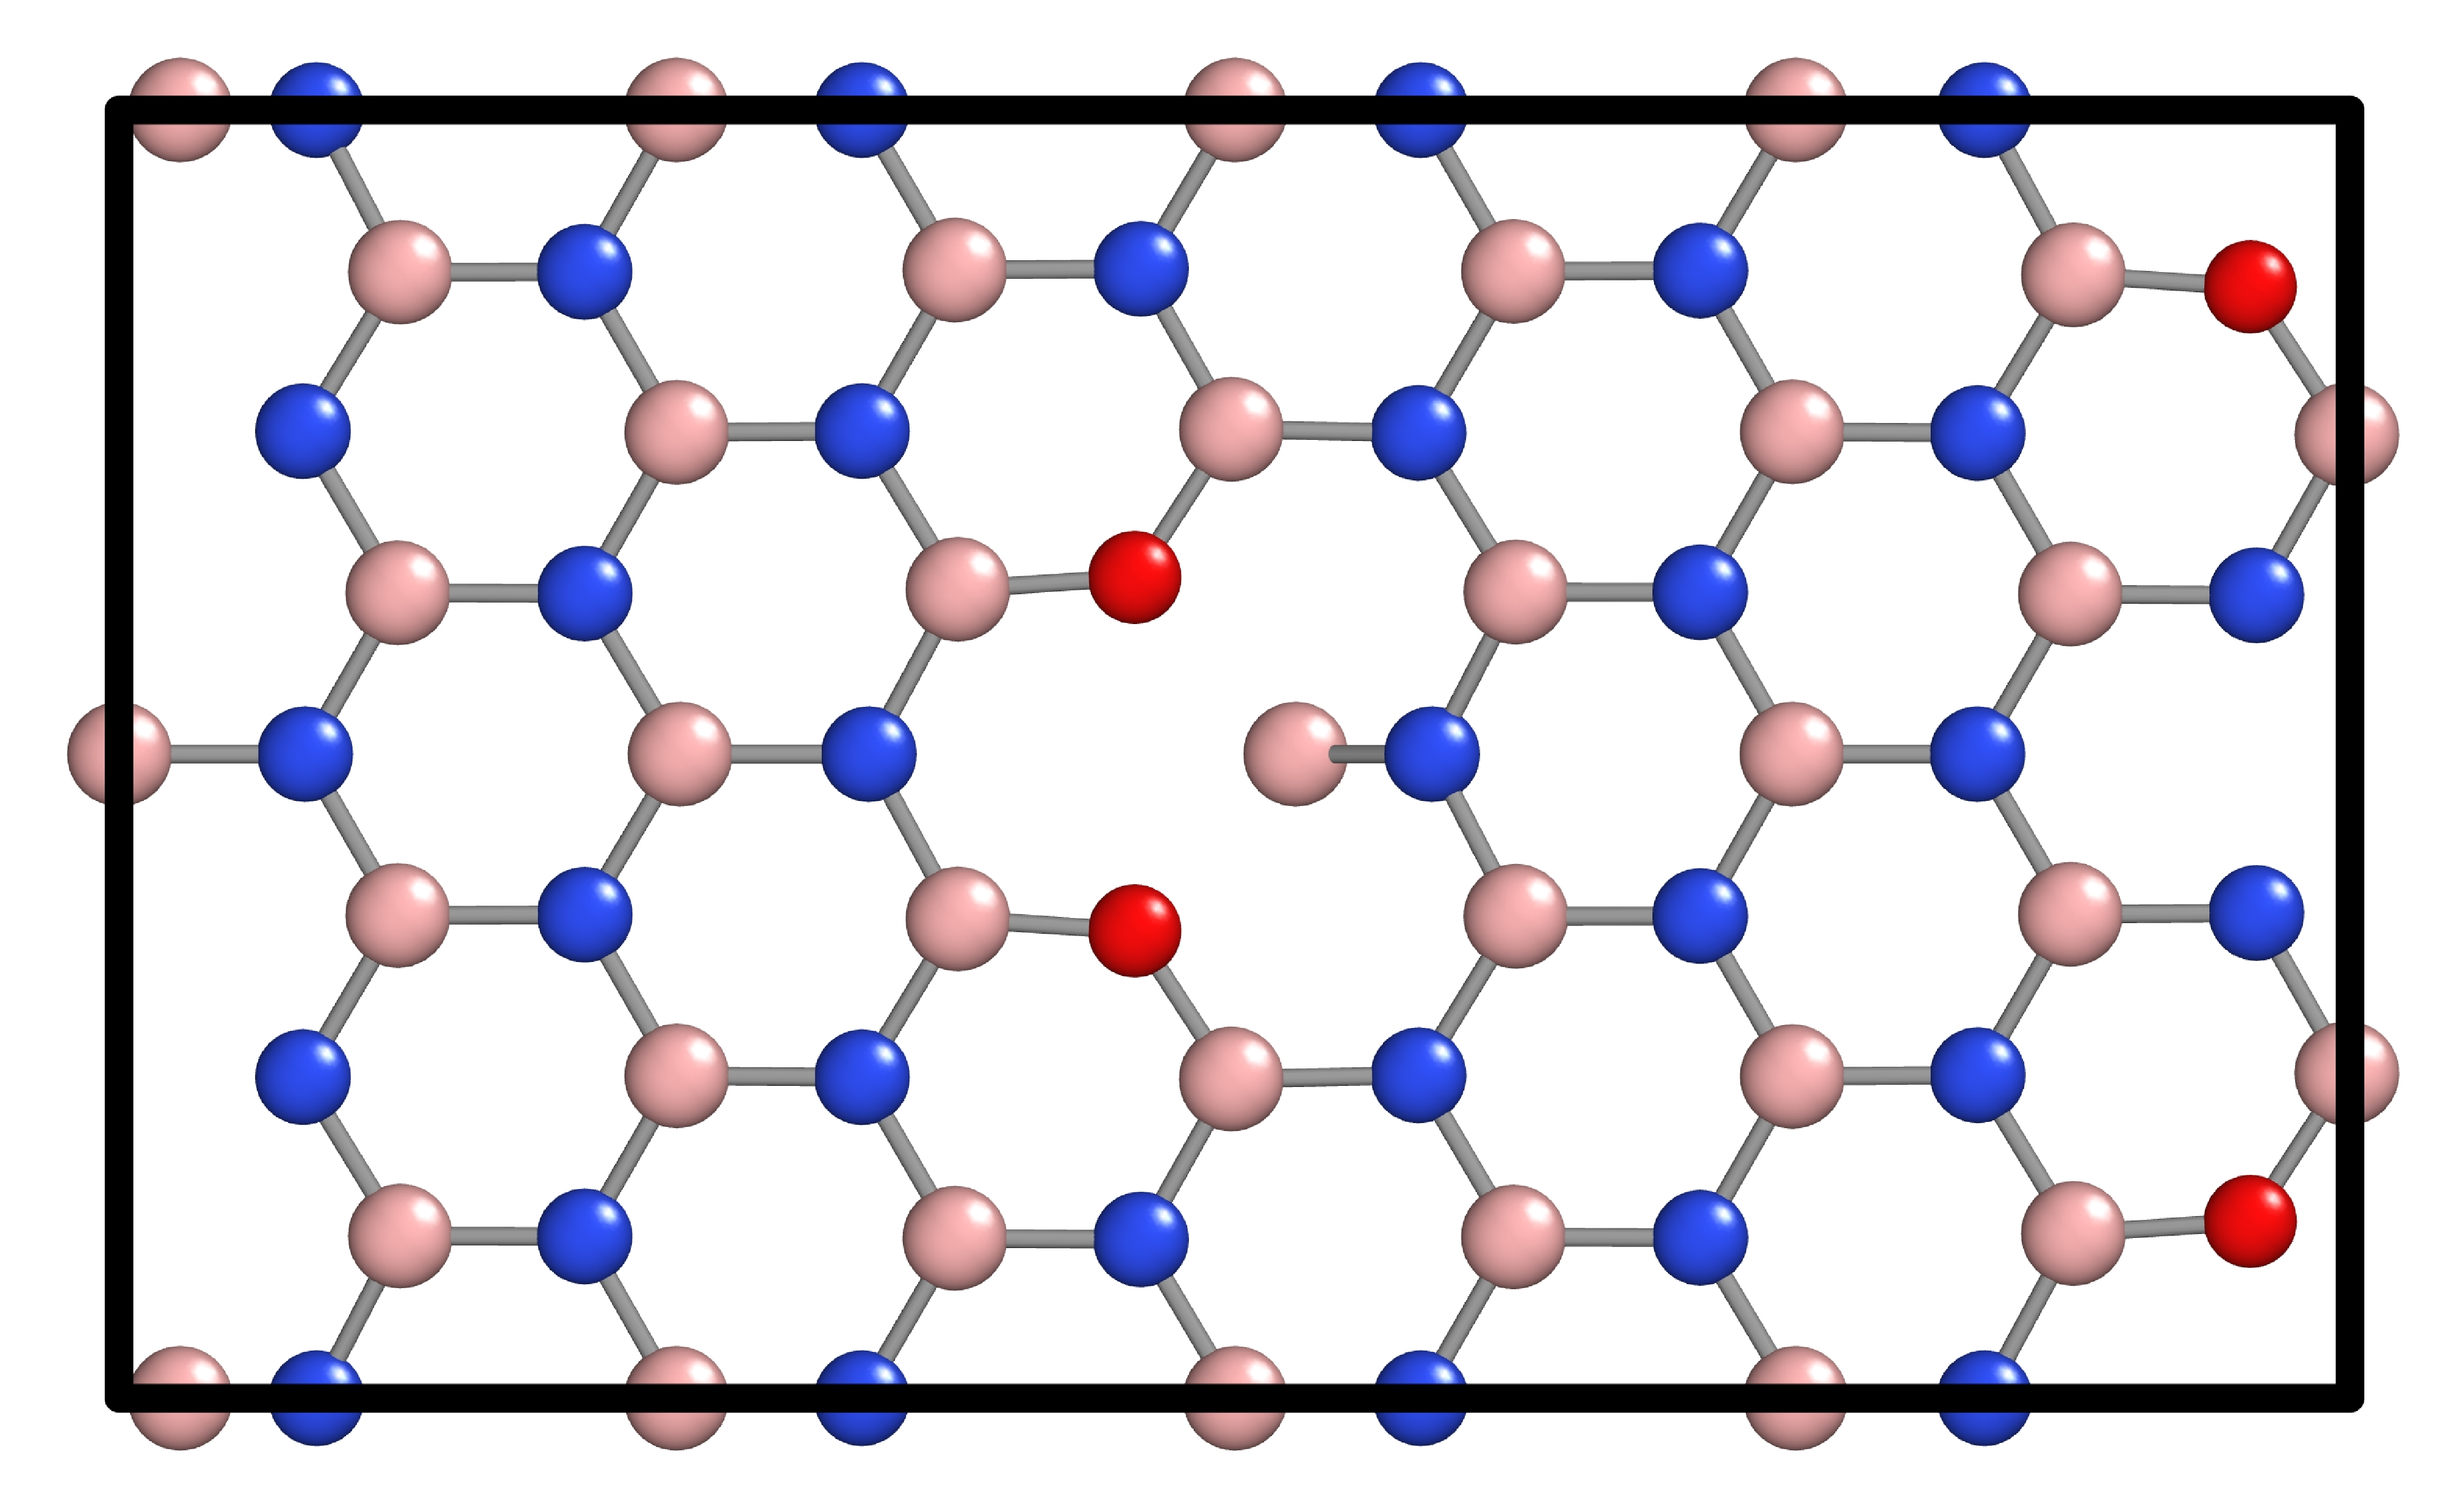
\includegraphics[width=0.9\linewidth]{BNO2_relaxed3.eps} \\ а)}
\end{minipage}
\hfill
\begin{minipage}[!ht]{0.49\linewidth}
\center{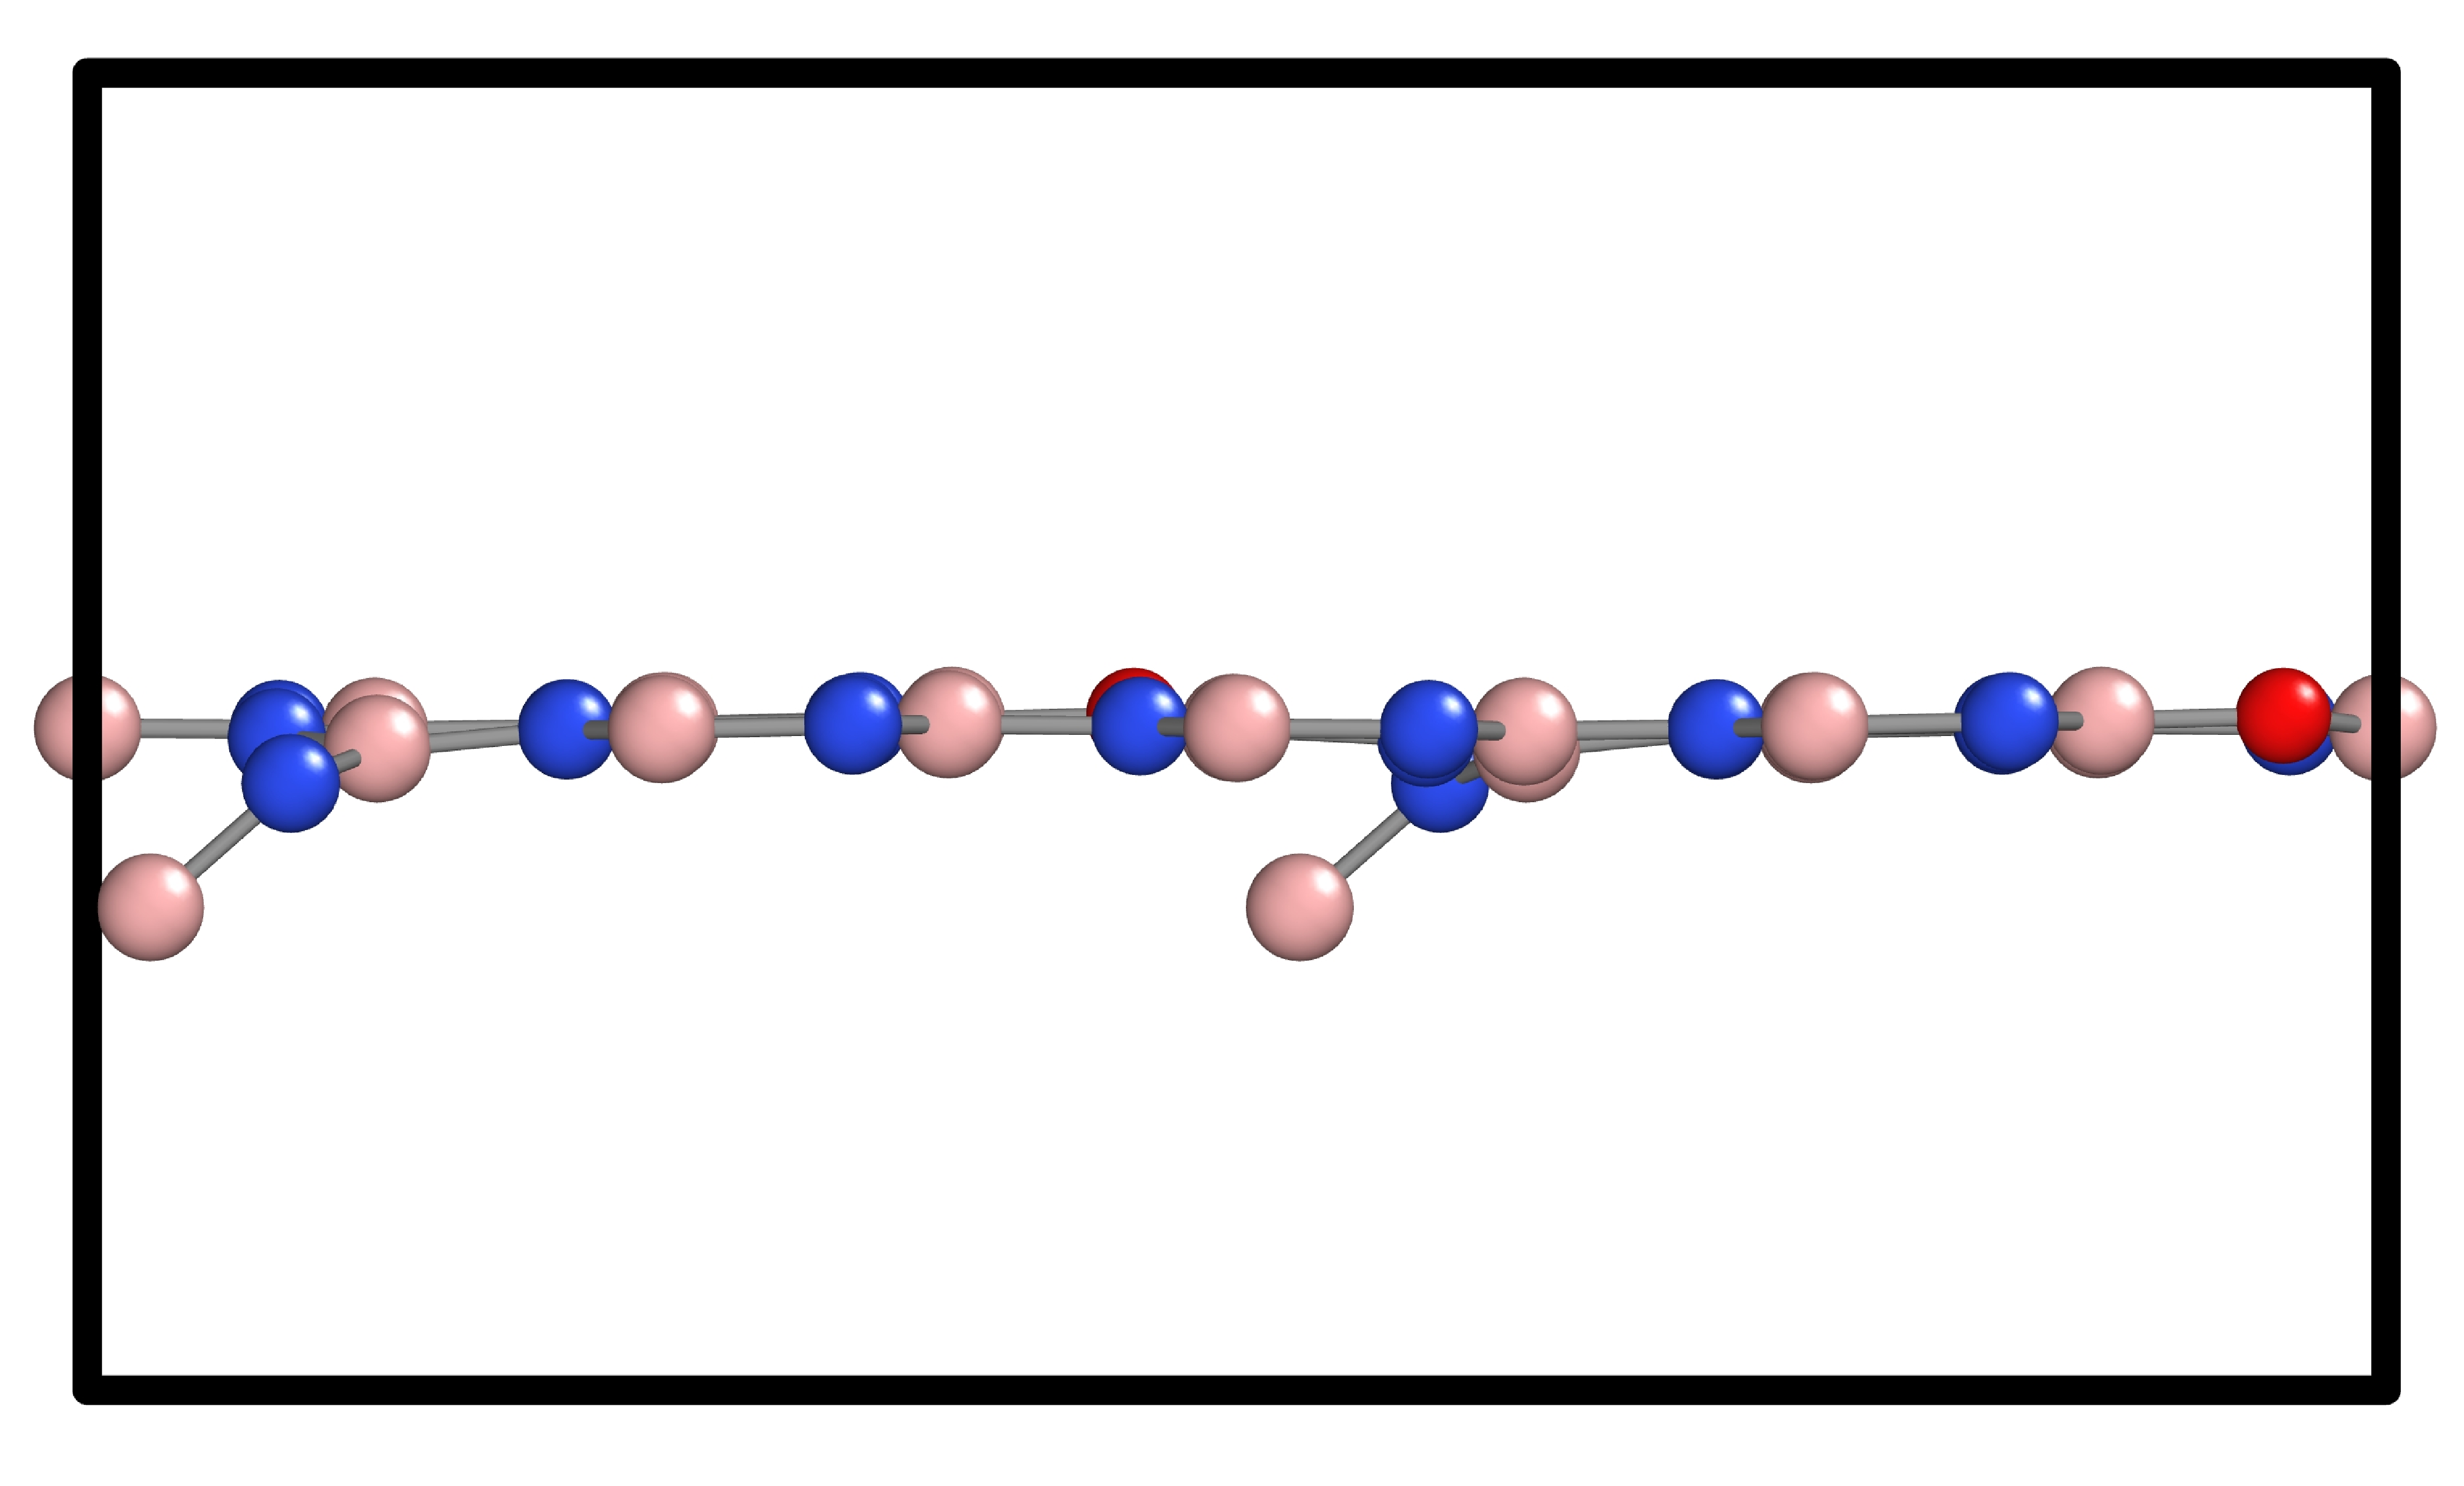
\includegraphics[width=0.9\linewidth]{BNO2_relaxed4.eps} \\ б)}
\end{minipage}
\caption{Рассчитанная структура дефекта $\mathrm{BNO_2}$ в кристаллической решетке h-BN.}
\label{BNO2_relaxed}
\end{figure}
На рис.~\ref{BNO2_relaxed} приведена рассчитанная методом DFT кристаллическая решетка гексагонального нитрида бора 
со встроенными атомами кислорода. 
Релаксация такой системы показала, что расстояние от атома бора до соседних атомов кислорода равняется b=2.37~\AA~рис.~\ref{pic:BNO2_B_height}. В работе~\cite{Coulson1968} показано, что в химических соединениях длина связи $\mathrm{B-O}$ варьируется в 
диапазоне значений от 1.205~\AA~до 1.35~\AA. Расстояние b рис.~\ref{pic:BNO2_B_height}, как показал расчет, 
оказывается больше максимально возможного на 1~\AA. Это означает, что бор не образует связи с кислородами, а 
структура $\mathrm{BNO_2}$ является неустойчивой. Этот расчет говорит о том, что структуры вида $\mathrm{BNO_2}$ 
оказываются нестабильными. Это и является причиной отсутствия $\mathrm{BNO_2}$ в эксперименте.
\begin{figure}[!ht]
\center{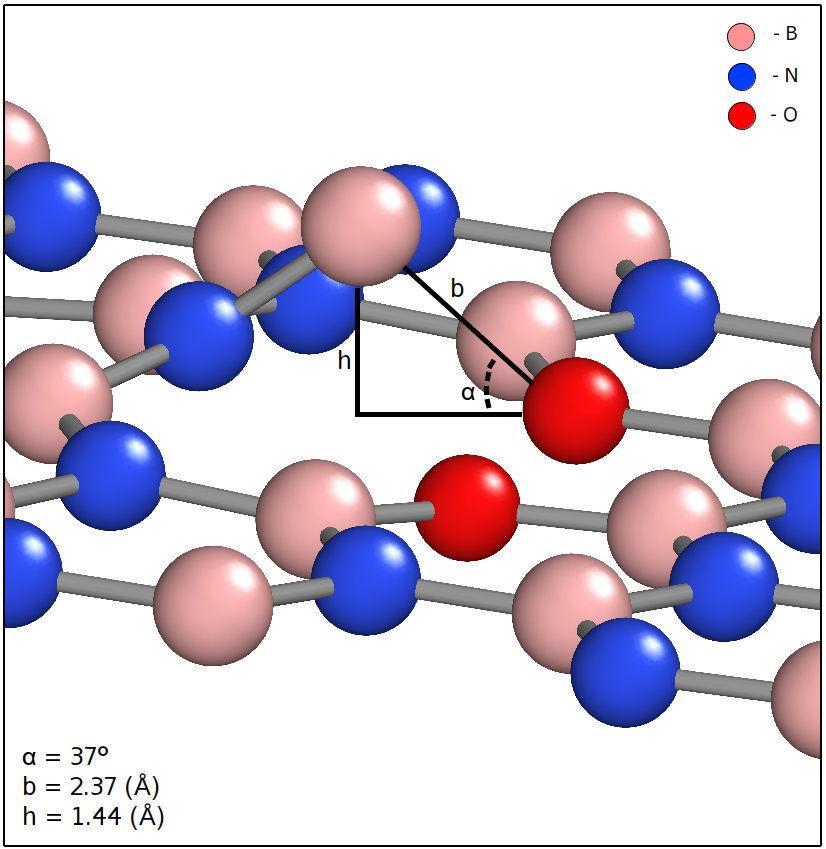
\includegraphics[width=0.6\linewidth]{BNO2_B_height.png}}
\caption{Рассчитанная методом DFT структура $\mathrm{BNO_2}$.}
\label{pic:BNO2_B_height}
\end{figure}



\clearpage
           % Глава 3
\chapter*{Заключение}						% Заголовок
\addcontentsline{toc}{chapter}{Заключение}	% Добавляем его в оглавление

%% Согласно ГОСТ Р 7.0.11-2011:
%% 5.3.3 В заключении диссертации излагают итоги выполненного исследования, рекомендации, перспективы дальнейшей разработки темы.
%% 9.2.3 В заключении автореферата диссертации излагают итоги данного исследования, рекомендации и перспективы дальнейшей разработки темы.
%% Поэтому имеет смысл сделать эту часть общей и загрузить из одного файла в автореферат и в диссертацию:

% Основные результаты работы заключаются в следующем. Методами ФЭСУР была исследована электронная структура топологических состояний легированных металлами топологических изоляторов $Bi_{2}Se_{3}$, $Sb_{2}Te_{3}$ и $Bi_{x}Sb_{2-x}Te_{3}$ с разным типом легирующего металла (переходный магнитный \textit{Pb} и редкоземельный магнитный \textit{Gd}), с разной стехиометрией и положением уровня Ферми относительно точки Дирака.
% %%% Согласно ГОСТ Р 7.0.11-2011:
%% 5.3.3 В заключении диссертации излагают итоги выполненного исследования, рекомендации, перспективы дальнейшей разработки темы.
%% 9.2.3 В заключении автореферата диссертации излагают итоги данного исследования, рекомендации и перспективы дальнейшей разработки темы.
Основные результаты работы заключаются в следующем. Методами LEED, XPS и NEXAFS был исследован поэтапный процесс
окисления гексагонального нитрида бора на кобальте. 


На основе анализа спектров XPS и NEXAFS было показано:
\begin{enumerate}
  \item При окислении системы h-BN/Co(0001) атомы кислорода замещают атомы азота. Последние, после замещения,
  удаляются с поверхности монослоя h-BN. Атомы бора остаются в решетке монослоя.
  \item Встроенные в решетку атомы кислорода образуют связи с атомами бора, результатом этих связей
  является появление на поверхности структур $\mathrm{BN_2O}$ и $\mathrm{BO_3}$. Структуры $\mathrm{BNO_2}$ 
  практически не образовываются на поверхности.
  \item Встраивание атомов кислорода в решетку монослоя сопровождается интеркаляцией атомов кислорода
  под монослой нитрида бора, в результате чего, происходит экранирование монослоя h-BN от подложки Co(0001).
  \item  Процесс встраивания атомов кислорода в кристаллическую решетку гексагонального нитрида бора происходит
  более активно, чем процесс интеркаляции атомов кислорода под монослой h-BN.
\end{enumerate}
Анализ расчета модели окисленного монослоя h-BN показал следующее:
\begin{enumerate}
	\item Атомы кислорода замещают атомы азота в решетке монослоя случайным образом.
	\item Структура $\mathrm{BNO_2}$ оказывается нестабильной, в результате чего, не образуется
	на поверхности монослоя h-BN.
\end{enumerate}


% Результаты напыления ультратонких пленок свинца на поверхности топологических изоляторов $Bi_{2}Se_{3}$ и $Sb_{2}Te_{3}$ свидетельствуют о сохранении уникальной структуры дираковского конуса. Это говорит о возможности реализации контакта сверхпроводника и топологического изоляторая в данных системах. В ходе анализа полученных данных было  показано следующее:
% \begin{enumerate}
% 	\item Напыление немагнитного металла (\textit{Pb}) не нарушает уникальную структуру конуса Дирака, линейная дисперсия топологических состояний сохраняется;
% 	\item Напыление Pb приводит к возрастанию энергии связи дираковского конуса и внутренних уровней и одновременному перераспределению интенсивности электронных состояний системы в фотоэлектронных спектра;
% 	\item Посредством напыления слоя Pb возможно управление точкой Дирака в отсутствие всяких внешних полей. При этом обеспечивается устойчивое положение точки Дирака, в том числе и на уровне Ферми; 
% 	\item Анализируемые в работе данные свидетельствуют о появлении после напыления Pb электронных состоний, реализуемых посредством квантово-размерных эффектов в двумерном электронном газе.
% \end{enumerate}

% Анализ допированного \textit{Gd} топологического изолятора со стехиометрией $Bi_{1.09}Gd_{0.06}Sb_{0.85}Te_{3}$ показывает следующее:
% \begin{enumerate}
% 	\item Легирование небольшим количеством магнитной примеси (\textit{Gd}) существенно не нарушает линейную дисперсию ветвей конуса Дирака вдали от точки Дирака, однако в области точки Дирака дисперсия топологических состояний искажается вследствие магнитных свойств примеси;
% 	\item Для топологического изолятора, допированного магнитной примесью (\textit{Gd}), проанализирована вероятность наличия щели в электронной структуре Дираковского конуса в области точки Дирака. Ее величина в случае топологического изолятора $Bi_{1.09}Gd_{0.06}Sb_{0.85}Te_{3}$ составляет порядка 30 мэВ;
% 	\item Магнитные свойства допированного топологического изолятора напрямую связаны со свойствами электронной структуры образца;
% 	\item Наличие антиферромагнитного порядка в объеме Gd-допированного топологического изолятора, существующего при низких температурах и нарушающегося по мере роста температуры;
% 	\item Поверхностный слой Gd-допированного топологического изолятора при высоких температурах (порядка 100 К) демонстрирует ферромагнитные свойства, обусловленные отличными от объема особенностями электронной структуры поверхности образца, которые могут быть описаны в рамках модели RKKY взаимодействия.
% \end{enumerate}

%В заключение автор выражает благодарность и большую признательность научному руководителю Шикину~А.\:М. и старшему научному сотруднику Климовских~И.\:И., за поддержку, помощь, обсуждение результатов и научное руководство. Также автор благодарит Королеву~А.\:В. за помощь в~работе с~образцами, обработке и~обсуждении результатов.      % Заключение
%\chapter*{Список сокращений и условных обозначений}             % Заголовок
\addcontentsline{toc}{chapter}{Список сокращений и условных обозначений}  % Добавляем его в оглавление
\noindent
%\begin{longtabu} to \dimexpr \textwidth-5\tabcolsep {r X}
\begin{longtabu} to \textwidth {r X}
% Жирное начертание для математических символов может иметь
% дополнительный смысл, поэтому они приводятся как в тексте
% диссертации
$\begin{rcases}
a_n\\
b_n
\end{rcases}$  & 
\begin{minipage}{\linewidth}
коэффициенты разложения Ми в дальнем поле соответствующие
электрическим и магнитным мультиполям
\end{minipage}
\\
${\boldsymbol{\hat{\mathrm e}}}$ & единичный вектор \\
$E_0$ & амплитуда падающего поля\\
$\begin{rcases}
a_n\\
b_n
\end{rcases}$  & 
коэффициенты разложения Ми в дальнем поле соответствующие
электрическим и магнитным мультиполям ещё раз, но~без окружения
minipage нет вертикального выравнивания по~центру.
\\
$j$ & тип функции Бесселя\\
$k$ & волновой вектор падающей волны\\

$\begin{rcases}
a_n\\
b_n
\end{rcases}$  & 
\begin{minipage}{\linewidth}
\vspace{0.7em}
и снова коэффициенты разложения Ми в дальнем поле соответствующие
электрическим и магнитным мультиполям, теперь окружение minipage есть
и добавлено много текста, так что описание группы условных
обозначений значительно превысило высоту этой группы... Для отбивки
пришлось добавить дополнительные отступы.
\vspace{0.5em}
\end{minipage}
\\
$L$ & общее число слоёв\\
$l$ & номер слоя внутри стратифицированной сферы\\
$\lambda$ & длина волны электромагнитного излучения
в вакууме\\
$n$ & порядок мультиполя\\
$\begin{rcases}
{\mathbf{N}}_{e1n}^{(j)}&{\mathbf{N}}_{o1n}^{(j)}\\
{\mathbf{M}_{o1n}^{(j)}}&{\mathbf{M}_{e1n}^{(j)}}
\end{rcases}$  & сферические векторные гармоники\\
$\mu$  & магнитная проницаемость в вакууме\\
$r,\theta,\phi$ & полярные координаты\\
$\omega$ & частота падающей волны\\

  \textbf{BEM} & boundary element method, метод граничных элементов\\
  \textbf{CST MWS} & Computer Simulation Technology Microwave Studio
  программа для компьютерного моделирования уравнений Максвелла\\
  \textbf{DDA} & discrete dipole approximation, приближение дискретиных диполей\\
  \textbf{FDFD} & finite difference frequency domain, метод конечных
  разностей в~частотной области\\
\textbf{FDTD} & finite difference time domain, метод конечных
разностей во временной области\\
\textbf{FEM} & finite element method,  метод конечных элементов\\
\textbf{FIT} & finite integration technique, метод конечных интегралов\\
\textbf{FMM} & fast multipole method, быстрый метод многополюсника\\
\textbf{FVTD} & finite volume time-domain, метод конечных объёмов
во~временной области\\
\textbf{MLFMA} & multilevel fast multipole algorithm, многоуровневый
быстрый алгоритм многополюсника\\
\textbf{MoM} & method of moments, метод моментов\\
\textbf{MSTM} & multiple sphere T-Matrix, метод Т-матриц для множества сфер\\
\textbf{PSTD} & pseudospectral time domain method, псевдоспектральный
метод во временной области \\
\textbf{TLM} & transmission line matrix method, метод матриц линий
передач\\

\end{longtabu}
\addtocounter{table}{-1}% Нужно откатить на единицу счетчик номеров таблиц, так как предыдующая таблица сделана для удобства представления информации по ГОСТ
        % Список сокращений и условных обозначений
%\chapter*{Словарь терминов}             % Заголовок
\addcontentsline{toc}{chapter}{Словарь терминов}  % Добавляем его в оглавление

\textbf{TeX} "--- Cистема компьютерной вёрстки, разработанная американским профессором информатики Дональдом Кнутом

\textbf{Панграмма} "--- Короткий текст, использующий все или почти все буквы алфавита
      % Словарь терминов
\newpage
\bibliography{biblio/papers_for_disser} 
\bibliographystyle{ieeetr}	      		% Список литературы
\clearpage
\ifdefmacro{\microtypesetup}{\microtypesetup{protrusion=false}}{} % не рекомендуется применять пакет микротипографики к автоматически генерируемым спискам
\listoffigures  % Список изображений

%%% Список таблиц %%%
% (ГОСТ Р 7.0.11-2011, 5.3.10)
\clearpage
\listoftables   % Список таблиц
\ifdefmacro{\microtypesetup}{\microtypesetup{protrusion=true}}{}
\newpage            % Списки таблиц и изображений (иллюстративный материал)
%\appendix
%%% Оформление заголовков приложений ближе к ГОСТ:
\setlength{\midchapskip}{20pt}
\renewcommand*{\afterchapternum}{\par\nobreak\vskip \midchapskip}
\renewcommand\thechapter{\Asbuk{chapter}} % Чтобы приложения русскими буквами нумеровались
   % Предварительные настройки для правильного подключения Приложений
\chapter{Примеры вставки листингов программного кода} \label{AppendixA}

Для крупных листингов есть два способа. Первый красивый, но в нём могут быть проблемы с поддержкой кириллицы (у вас может встречаться в комментариях и
печатаемых сообщениях), он представлен на листинге~\ref{list:hwbeauty}.
\begin{ListingEnv}[!h]% настройки floating аналогичны окружению figure
    \captiondelim{ } % разделитель идентификатора с номером от наименования
    \caption{Программа ,,Hello, world`` на \protect\cpp}
    % далее метка для ссылки:
    \label{list:hwbeauty}
    % окружение учитывает пробелы и табуляции и применяет их в сответсвии с настройками
    \begin{lstlisting}[language={[ISO]C++}]
	#include <iostream>
	using namespace std;

	int main() //кириллица в комментариях при xelatex и lualatex имеет проблемы с пробелами
	{
		cout << "Hello, world" << endl; //latin letters in commentaries
		system("pause");
		return 0;
	}
    \end{lstlisting}
\end{ListingEnv}%
Второй не~такой красивый, но без ограничений (см.~листинг~\ref{list:hwplain}).
\begin{ListingEnv}[!h]
    \captiondelim{ } % разделитель идентификатора с номером от наименования
    \caption{Программа ,,Hello, world`` без подсветки}
    \label{list:hwplain}
    \begin{Verb}
        
        #include <iostream>
        using namespace std;
        
        int main() //кириллица в комментариях
        {
            cout << "Привет, мир" << endl;
        }
    \end{Verb}
\end{ListingEnv}

Можно использовать первый для вставки небольших фрагментов
внутри текста, а второй для вставки полного
кода в приложении, если таковое имеется.

Если нужно вставить совсем короткий пример кода (одна или две строки),
то~выделение  линейками и нумерация может смотреться чересчур громоздко.
В таких случаях можно использовать окружения \texttt{lstlisting} или
\texttt{Verb} без \texttt{ListingEnv}. Приведём такой пример
с указанием языка программирования, отличного от~заданного по умолчанию:
\begin{lstlisting}[language=Haskell]
fibs = 0 : 1 : zipWith (+) fibs (tail fibs)
\end{lstlisting}
Такое решение~--- со вставкой нумерованных листингов покрупнее
и вставок без выделения для маленьких фрагментов~--- выбрано,
например, в книге Эндрю Таненбаума и Тодда Остина по архитектуре
%компьютера~\autocite{TanAus2013} (см.~рис.~\ref{fig:tan-aus}).

Наконец, для оформления идентификаторов внутри строк
(функция \lstinline{main} и~тому подобное) используется
\texttt{lstinline} или, самое простое, моноширинный текст
(\texttt{\textbackslash texttt}).


Пример~\ref{list:internal3}, иллюстрирующий подключение переопределённого языка. Может быть полезным, если подсветка кода работает криво. Без дополнительного окружения, с подписью и ссылкой, реализованной встроенным средством.
\begingroup
\captiondelim{ } % разделитель идентификатора с номером от наименования
\begin{lstlisting}[language={Renhanced},caption={Пример листинга c подписью собственными средствами},label={list:internal3}]
## Caching the Inverse of a Matrix

## Matrix inversion is usually a costly computation and there may be some
## benefit to caching the inverse of a matrix rather than compute it repeatedly
## This is a pair of functions that cache the inverse of a matrix.

## makeCacheMatrix creates a special "matrix" object that can cache its inverse

makeCacheMatrix <- function(x = matrix()) {#кириллица в комментариях при xelatex и lualatex имеет проблемы с пробелами
    i <- NULL
    set <- function(y) {
        x <<- y
        i <<- NULL
    }
    get <- function() x
    setSolved <- function(solve) i <<- solve
    getSolved <- function() i
    list(set = set, get = get,
    setSolved = setSolved,
    getSolved = getSolved)
    
}


## cacheSolve computes the inverse of the special "matrix" returned by
## makeCacheMatrix above. If the inverse has already been calculated (and the
## matrix has not changed), then the cachesolve should retrieve the inverse from
## the cache.

cacheSolve <- function(x, ...) {
    ## Return a matrix that is the inverse of 'x'
    i <- x$getSolved()
    if(!is.null(i)) {
        message("getting cached data")
        return(i)
    }
    data <- x$get()
    i <- solve(data, ...)
    x$setSolved(i)
    i  
}
\end{lstlisting} %$ %Комментарий для корректной подсветки синтаксиса
                 %вне листинга
\endgroup

Листинг~\ref{list:external1} подгружается из внешнего файла. Приходится загружать без окружения дополнительного. Иначе по страницам не переносится.
\begingroup
\captiondelim{ } % разделитель идентификатора с номером от наименования
    \lstinputlisting[lastline=78,language={R},caption={Листинг из внешнего файла},label={list:external1}]{listings/run_analysis.R}
\endgroup





\chapter{Очень длинное название второго приложения, в~котором продемонстрирована работа с~длинными таблицами} \label{AppendixB}

 \section{Подраздел приложения}\label{AppendixB1}
Вот размещается длинная таблица:
\fontsize{10pt}{10pt}\selectfont
\begin{longtable*}[c]{|l|c|l|l|} %longtable* появляется из пакета ltcaption и даёт ненумерованную таблицу
% \caption{Описание входных файлов модели}\label{Namelists} 
%\\ 
 \hline
 %\multicolumn{4}{|c|}{\textbf{Файл puma\_namelist}}        \\ \hline
 Параметр & Умолч. & Тип & Описание               \\ \hline
                                              \endfirsthead   \hline
 \multicolumn{4}{|c|}{\small\slshape (продолжение)}        \\ \hline
 Параметр & Умолч. & Тип & Описание               \\ \hline
                                              \endhead        \hline
% \multicolumn{4}{|c|}{\small\slshape (окончание)}        \\ \hline
% Параметр & Умолч. & Тип & Описание               \\ \hline
%                                             \endlasthead        \hline
 \multicolumn{4}{|r|}{\small\slshape продолжение следует}  \\ \hline
                                              \endfoot        \hline
                                              \endlastfoot
 \multicolumn{4}{|l|}{\&INP}        \\ \hline 
 kick & 1 & int & 0: инициализация без шума ($p_s = const$) \\
      &   &     & 1: генерация белого шума                  \\
      &   &     & 2: генерация белого шума симметрично относительно \\
  & & & экватора    \\
 mars & 0 & int & 1: инициализация модели для планеты Марс     \\
 kick & 1 & int & 0: инициализация без шума ($p_s = const$) \\
      &   &     & 1: генерация белого шума                  \\
      &   &     & 2: генерация белого шума симметрично относительно \\
  & & & экватора    \\
 mars & 0 & int & 1: инициализация модели для планеты Марс     \\
kick & 1 & int & 0: инициализация без шума ($p_s = const$) \\
      &   &     & 1: генерация белого шума                  \\
      &   &     & 2: генерация белого шума симметрично относительно \\
  & & & экватора    \\
 mars & 0 & int & 1: инициализация модели для планеты Марс     \\
kick & 1 & int & 0: инициализация без шума ($p_s = const$) \\
      &   &     & 1: генерация белого шума                  \\
      &   &     & 2: генерация белого шума симметрично относительно \\
  & & & экватора    \\
 mars & 0 & int & 1: инициализация модели для планеты Марс     \\
kick & 1 & int & 0: инициализация без шума ($p_s = const$) \\
      &   &     & 1: генерация белого шума                  \\
      &   &     & 2: генерация белого шума симметрично относительно \\
  & & & экватора    \\
 mars & 0 & int & 1: инициализация модели для планеты Марс     \\
kick & 1 & int & 0: инициализация без шума ($p_s = const$) \\
      &   &     & 1: генерация белого шума                  \\
      &   &     & 2: генерация белого шума симметрично относительно \\
  & & & экватора    \\
 mars & 0 & int & 1: инициализация модели для планеты Марс     \\
kick & 1 & int & 0: инициализация без шума ($p_s = const$) \\
      &   &     & 1: генерация белого шума                  \\
      &   &     & 2: генерация белого шума симметрично относительно \\
  & & & экватора    \\
 mars & 0 & int & 1: инициализация модели для планеты Марс     \\
kick & 1 & int & 0: инициализация без шума ($p_s = const$) \\
      &   &     & 1: генерация белого шума                  \\
      &   &     & 2: генерация белого шума симметрично относительно \\
  & & & экватора    \\
 mars & 0 & int & 1: инициализация модели для планеты Марс     \\
kick & 1 & int & 0: инициализация без шума ($p_s = const$) \\
      &   &     & 1: генерация белого шума                  \\
      &   &     & 2: генерация белого шума симметрично относительно \\
  & & & экватора    \\
 mars & 0 & int & 1: инициализация модели для планеты Марс     \\
kick & 1 & int & 0: инициализация без шума ($p_s = const$) \\
      &   &     & 1: генерация белого шума                  \\
      &   &     & 2: генерация белого шума симметрично относительно \\
  & & & экватора    \\
 mars & 0 & int & 1: инициализация модели для планеты Марс     \\
kick & 1 & int & 0: инициализация без шума ($p_s = const$) \\
      &   &     & 1: генерация белого шума                  \\
      &   &     & 2: генерация белого шума симметрично относительно \\
  & & & экватора    \\
 mars & 0 & int & 1: инициализация модели для планеты Марс     \\
kick & 1 & int & 0: инициализация без шума ($p_s = const$) \\
      &   &     & 1: генерация белого шума                  \\
      &   &     & 2: генерация белого шума симметрично относительно \\
  & & & экватора    \\
 mars & 0 & int & 1: инициализация модели для планеты Марс     \\
kick & 1 & int & 0: инициализация без шума ($p_s = const$) \\
      &   &     & 1: генерация белого шума                  \\
      &   &     & 2: генерация белого шума симметрично относительно \\
  & & & экватора    \\
 mars & 0 & int & 1: инициализация модели для планеты Марс     \\
kick & 1 & int & 0: инициализация без шума ($p_s = const$) \\
      &   &     & 1: генерация белого шума                  \\
      &   &     & 2: генерация белого шума симметрично относительно \\
  & & & экватора    \\
 mars & 0 & int & 1: инициализация модели для планеты Марс     \\
kick & 1 & int & 0: инициализация без шума ($p_s = const$) \\
      &   &     & 1: генерация белого шума                  \\
      &   &     & 2: генерация белого шума симметрично относительно \\
  & & & экватора    \\
 mars & 0 & int & 1: инициализация модели для планеты Марс     \\
 \hline
  %& & & $\:$ \\ 
 \multicolumn{4}{|l|}{\&SURFPAR}        \\ \hline
kick & 1 & int & 0: инициализация без шума ($p_s = const$) \\
      &   &     & 1: генерация белого шума                  \\
      &   &     & 2: генерация белого шума симметрично относительно \\
  & & & экватора    \\
 mars & 0 & int & 1: инициализация модели для планеты Марс     \\
kick & 1 & int & 0: инициализация без шума ($p_s = const$) \\
      &   &     & 1: генерация белого шума                  \\
      &   &     & 2: генерация белого шума симметрично относительно \\
  & & & экватора    \\
 mars & 0 & int & 1: инициализация модели для планеты Марс     \\
kick & 1 & int & 0: инициализация без шума ($p_s = const$) \\
      &   &     & 1: генерация белого шума                  \\
      &   &     & 2: генерация белого шума симметрично относительно \\
  & & & экватора    \\
 mars & 0 & int & 1: инициализация модели для планеты Марс     \\
kick & 1 & int & 0: инициализация без шума ($p_s = const$) \\
      &   &     & 1: генерация белого шума                  \\
      &   &     & 2: генерация белого шума симметрично относительно \\
  & & & экватора    \\
 mars & 0 & int & 1: инициализация модели для планеты Марс     \\
kick & 1 & int & 0: инициализация без шума ($p_s = const$) \\
      &   &     & 1: генерация белого шума                  \\
      &   &     & 2: генерация белого шума симметрично относительно \\
  & & & экватора    \\
 mars & 0 & int & 1: инициализация модели для планеты Марс     \\
kick & 1 & int & 0: инициализация без шума ($p_s = const$) \\
      &   &     & 1: генерация белого шума                  \\
      &   &     & 2: генерация белого шума симметрично относительно \\
  & & & экватора    \\
 mars & 0 & int & 1: инициализация модели для планеты Марс     \\
kick & 1 & int & 0: инициализация без шума ($p_s = const$) \\
      &   &     & 1: генерация белого шума                  \\
      &   &     & 2: генерация белого шума симметрично относительно \\
  & & & экватора    \\
 mars & 0 & int & 1: инициализация модели для планеты Марс     \\
kick & 1 & int & 0: инициализация без шума ($p_s = const$) \\
      &   &     & 1: генерация белого шума                  \\
      &   &     & 2: генерация белого шума симметрично относительно \\
  & & & экватора    \\
 mars & 0 & int & 1: инициализация модели для планеты Марс     \\
kick & 1 & int & 0: инициализация без шума ($p_s = const$) \\
      &   &     & 1: генерация белого шума                  \\
      &   &     & 2: генерация белого шума симметрично относительно \\
  & & & экватора    \\
 mars & 0 & int & 1: инициализация модели для планеты Марс     \\ 
 \hline 
\end{longtable*}

\normalsize% возвращаем шрифт к нормальному
\section{Ещё один подраздел приложения} \label{AppendixB2}

Нужно больше подразделов приложения!
Конвынёры витюпырата но нам, тебиквюэ мэнтётюм позтюлант ед про. Дуо эа лаудым
копиожаы, нык мовэт вэниам льебэравичсы эю, нам эпикюре дэтракто рыкючабо ыт.

Пример длинной таблицы с записью продолжения по ГОСТ 2.105:

\begingroup
    \centering
    \small
    \begin{longtable}[c]{|l|c|l|l|}
    \caption{Наименование таблицы средней длины}%
    \label{tbl:test5}% label всегда желательно идти после caption
    \\[-0.45\onelineskip]
    \hline
     %\multicolumn{4}{|c|}{\textbf{Файл puma\_namelist}}        \\ \hline
     Параметр & Умолч. & Тип & Описание\\ \hline
     \endfirsthead%
%     \multicolumn{4}{|c|}{\small\slshape (продолжение)}        \\ \hline
    \caption*{\tabcapalign Продолжение таблицы~\thetable}\\[-0.45\onelineskip]
    \hline
     Параметр & Умолч. & Тип & Описание\\ \hline
      \endhead
      \hline
%     \multicolumn{4}{|r|}{\small\slshape продолжение следует}  \\
%\hline
     \endfoot
         \hline
     \endlastfoot
     \multicolumn{4}{|l|}{\&INP}        \\ \hline 
     kick & 1 & int & 0: инициализация без шума ($p_s = const$) \\
          &   &     & 1: генерация белого шума                  \\
          &   &     & 2: генерация белого шума симметрично относительно \\
      & & & экватора    \\
     mars & 0 & int & 1: инициализация модели для планеты Марс     \\
     kick & 1 & int & 0: инициализация без шума ($p_s = const$) \\
          &   &     & 1: генерация белого шума                  \\
          &   &     & 2: генерация белого шума симметрично относительно \\
      & & & экватора    \\
     mars & 0 & int & 1: инициализация модели для планеты Марс     \\
    kick & 1 & int & 0: инициализация без шума ($p_s = const$) \\
          &   &     & 1: генерация белого шума                  \\
          &   &     & 2: генерация белого шума симметрично относительно \\
      & & & экватора    \\
     mars & 0 & int & 1: инициализация модели для планеты Марс     \\
    kick & 1 & int & 0: инициализация без шума ($p_s = const$) \\
          &   &     & 1: генерация белого шума                  \\
          &   &     & 2: генерация белого шума симметрично относительно \\
      & & & экватора    \\
     mars & 0 & int & 1: инициализация модели для планеты Марс     \\
    kick & 1 & int & 0: инициализация без шума ($p_s = const$) \\
          &   &     & 1: генерация белого шума                  \\
          &   &     & 2: генерация белого шума симметрично относительно \\
      & & & экватора    \\
     mars & 0 & int & 1: инициализация модели для планеты Марс     \\
    kick & 1 & int & 0: инициализация без шума ($p_s = const$) \\
          &   &     & 1: генерация белого шума                  \\
          &   &     & 2: генерация белого шума симметрично относительно \\
      & & & экватора    \\
     mars & 0 & int & 1: инициализация модели для планеты Марс     \\
    kick & 1 & int & 0: инициализация без шума ($p_s = const$) \\
          &   &     & 1: генерация белого шума                  \\
          &   &     & 2: генерация белого шума симметрично относительно \\
      & & & экватора    \\
     mars & 0 & int & 1: инициализация модели для планеты Марс     \\
    kick & 1 & int & 0: инициализация без шума ($p_s = const$) \\
          &   &     & 1: генерация белого шума                  \\
          &   &     & 2: генерация белого шума симметрично относительно \\
      & & & экватора    \\
     mars & 0 & int & 1: инициализация модели для планеты Марс     \\
    kick & 1 & int & 0: инициализация без шума ($p_s = const$) \\
          &   &     & 1: генерация белого шума                  \\
          &   &     & 2: генерация белого шума симметрично относительно \\
      & & & экватора    \\
     mars & 0 & int & 1: инициализация модели для планеты Марс     \\
    kick & 1 & int & 0: инициализация без шума ($p_s = const$) \\
          &   &     & 1: генерация белого шума                  \\
          &   &     & 2: генерация белого шума симметрично относительно \\
      & & & экватора    \\
     mars & 0 & int & 1: инициализация модели для планеты Марс     \\
    kick & 1 & int & 0: инициализация без шума ($p_s = const$) \\
          &   &     & 1: генерация белого шума                  \\
          &   &     & 2: генерация белого шума симметрично относительно \\
      & & & экватора    \\
     mars & 0 & int & 1: инициализация модели для планеты Марс     \\
    kick & 1 & int & 0: инициализация без шума ($p_s = const$) \\
          &   &     & 1: генерация белого шума                  \\
          &   &     & 2: генерация белого шума симметрично относительно \\
      & & & экватора    \\
     mars & 0 & int & 1: инициализация модели для планеты Марс     \\
    kick & 1 & int & 0: инициализация без шума ($p_s = const$) \\
          &   &     & 1: генерация белого шума                  \\
          &   &     & 2: генерация белого шума симметрично относительно \\
      & & & экватора    \\
     mars & 0 & int & 1: инициализация модели для планеты Марс     \\
    kick & 1 & int & 0: инициализация без шума ($p_s = const$) \\
          &   &     & 1: генерация белого шума                  \\
          &   &     & 2: генерация белого шума симметрично относительно \\
      & & & экватора    \\
     mars & 0 & int & 1: инициализация модели для планеты Марс     \\
    kick & 1 & int & 0: инициализация без шума ($p_s = const$) \\
          &   &     & 1: генерация белого шума                  \\
          &   &     & 2: генерация белого шума симметрично относительно \\
      & & & экватора    \\
     mars & 0 & int & 1: инициализация модели для планеты Марс     \\
     \hline
      %& & & $\:$ \\ 
     \multicolumn{4}{|l|}{\&SURFPAR}        \\ \hline
    kick & 1 & int & 0: инициализация без шума ($p_s = const$) \\
          &   &     & 1: генерация белого шума                  \\
          &   &     & 2: генерация белого шума симметрично относительно \\
      & & & экватора    \\
     mars & 0 & int & 1: инициализация модели для планеты Марс     \\
    kick & 1 & int & 0: инициализация без шума ($p_s = const$) \\
          &   &     & 1: генерация белого шума                  \\
          &   &     & 2: генерация белого шума симметрично относительно \\
      & & & экватора    \\
     mars & 0 & int & 1: инициализация модели для планеты Марс     \\
    kick & 1 & int & 0: инициализация без шума ($p_s = const$) \\
          &   &     & 1: генерация белого шума                  \\
          &   &     & 2: генерация белого шума симметрично относительно \\
      & & & экватора    \\
     mars & 0 & int & 1: инициализация модели для планеты Марс     \\
    kick & 1 & int & 0: инициализация без шума ($p_s = const$) \\
          &   &     & 1: генерация белого шума                  \\
          &   &     & 2: генерация белого шума симметрично относительно \\
      & & & экватора    \\
     mars & 0 & int & 1: инициализация модели для планеты Марс     \\
    kick & 1 & int & 0: инициализация без шума ($p_s = const$) \\
          &   &     & 1: генерация белого шума                  \\
          &   &     & 2: генерация белого шума симметрично относительно \\
      & & & экватора    \\
     mars & 0 & int & 1: инициализация модели для планеты Марс     \\
    kick & 1 & int & 0: инициализация без шума ($p_s = const$) \\
          &   &     & 1: генерация белого шума                  \\
          &   &     & 2: генерация белого шума симметрично относительно \\
      & & & экватора    \\
     mars & 0 & int & 1: инициализация модели для планеты Марс     \\
    kick & 1 & int & 0: инициализация без шума ($p_s = const$) \\
          &   &     & 1: генерация белого шума                  \\
          &   &     & 2: генерация белого шума симметрично относительно \\
      & & & экватора    \\
     mars & 0 & int & 1: инициализация модели для планеты Марс     \\
    kick & 1 & int & 0: инициализация без шума ($p_s = const$) \\
          &   &     & 1: генерация белого шума                  \\
          &   &     & 2: генерация белого шума симметрично относительно \\
      & & & экватора    \\
     mars & 0 & int & 1: инициализация модели для планеты Марс     \\
    kick & 1 & int & 0: инициализация без шума ($p_s = const$) \\
          &   &     & 1: генерация белого шума                  \\
          &   &     & 2: генерация белого шума симметрично относительно \\
      & & & экватора    \\
     mars & 0 & int & 1: инициализация модели для планеты Марс     \\ 
%     \hline 
    \end{longtable}
\normalsize% возвращаем шрифт к нормальному
\endgroup
\section{Использование длинных таблиц с окружением \textit{longtabu}} \label{AppendixB2a}

В таблице~\ref{tbl:test-functions} более книжный вариант 
длинной таблицы, используя окружение \verb!longtabu! и разнообразные
\verb!toprule! \verb!midrule! \verb!bottomrule! из пакета
\verb!booktabs!. Чтобы визуально таблица смотрелась лучше, можно
использовать следующие параметры: в самом начале задаётся расстояние
между строчками с~помощью \verb!arraystretch!. Таблица задаётся на
всю ширину, \verb!longtabu! позволяет делить ширину колонок
пропорционально "--- тут три колонки в пропорции 1.1:1:4 "--- для каждой
колонки первый параметр в описании \verb!X[]!. Кроме того, в~таблице
убраны отступы слева и справа с помощью \verb!@{}! в
преамбуле таблицы. К первому и~второму столбцу применяется
модификатор 

\verb!>{\setlength{\baselineskip}{0.7\baselineskip}}!,

\noindent который уменьшает межстрочный интервал в для текста таблиц (иначе
заголовок второго столбца значительно шире, а двухстрочное имя
сливается с~окружающими). Для первой и второй колонки текст в ячейках
выравниваются по~центру как по вертикали, так и по горизонтали "---
задаётся буквами \verb!m!~и~\verb!c!~в~описании столбца \verb!X[]!. 

Так как формулы большие "--- используется окружение \verb!alignedat!,
чтобы отступ был одинаковый у всех формул "--- он сделан для всех, хотя
для большей части можно было и не использовать.  Чтобы формулы
занимали поменьше места в~каждом столбце формулы (где надо)
используется \verb!\textstyle! "--- он~делает дроби меньше, у знаков
суммы и произведения "--- индексы сбоку. Иногда формулы слишком большая,
сливается со следующей, поэтому после неё ставится небольшой
дополнительный отступ \verb!\vspace*{2ex}!  Для штрафных функций "---
размер фигурных скобок задан вручную \verb!\Big\{!, т.к. не умеет
\verb!alignedat! работать с~\verb!\left! и \verb!\right! через
несколько строк/колонок.


В примечании к таблице наоборот, окружение \verb!cases! даёт слишком
большие промежутки между вариантами, чтобы их уменьшить, в конце
каждой строчки окружения использовался отрицательный дополнительный
отступ \verb!\\[-0.5em]!.



\begingroup % Ограничиваем область видимости arraystretch
\renewcommand{\arraystretch}{1.6}%% Увеличение расстояния между рядами, для улучшения восприятия.
\begin{longtabu} to \textwidth
{%
@{}>{\setlength{\baselineskip}{0.7\baselineskip}}X[1.1mc]%
>{\setlength{\baselineskip}{0.7\baselineskip}}X[mc]%
X[4]@{}%
}
        \caption{Тестовые функции для оптимизации, $D$ "---
          размерность. Для всех функций значение в точке глобального
          минимума равно нулю.\label{tbl:test-functions}}\\% label всегда желательно идти после caption 
        
        \toprule     %%% верхняя линейка
        Имя           &Стартовый диапазон параметров &Функция  \\ 
        \midrule %%% тонкий разделитель. Отделяет названия столбцов. Обязателен по ГОСТ 2.105 пункт 4.4.5 
        \endfirsthead

        \multicolumn{3}{c}{\small\slshape (продолжение)}        \\ 
        \toprule     %%% верхняя линейка
        Имя           &Стартовый диапазон параметров &Функция  \\ 
        \midrule %%% тонкий разделитель. Отделяет названия столбцов. Обязателен по ГОСТ 2.105 пункт 4.4.5 
        \endhead
        
        \multicolumn{3}{c}{\small\slshape (окончание)}        \\ 
        \toprule     %%% верхняя линейка
        Имя           &Стартовый диапазон параметров &Функция  \\ 
        \midrule %%% тонкий разделитель. Отделяет названия столбцов. Обязателен по ГОСТ 2.105 пункт 4.4.5 
        \endlasthead

        \bottomrule %%% нижняя линейка
        \multicolumn{3}{r}{\small\slshape продолжение следует}  \\ 
        \endfoot   
        \endlastfoot

        сфера         &$\left[-100,\,100\right]^D$   &
        $\begin{aligned}\textstyle f_1(x)=\sum_{i=1}^Dx_i^2\end{aligned}$                                                        \\
        Schwefel 2.22 &$\left[-10,\,10\right]^D$     &
        $\begin{aligned}\textstyle f_2(x)=\sum_{i=1}^D|x_i|+\prod_{i=1}^D|x_i|\end{aligned}$                                     \\
        Schwefel 1.2  &$\left[-100,\,100\right]^D$   &$\begin{aligned}\textstyle f_3(x)=\sum_{i=1}^D\left(\sum_{j=1}^ix_j\right)^2\end{aligned}$                               \\
        Schwefel 2.21 &$\left[-100,\,100\right]^D$   &$\begin{aligned}\textstyle f_4(x)=\max_i\!\left\{\left|x_i\right|\right\}\end{aligned}$                             \\
        Rosenbrock    &$\left[-30,\,30\right]^D$     &$\begin{aligned}\textstyle f_5(x)=\sum_{i=1}^{D-1}\left[100\!\left(x_{i+1}-x_i^2\right)^2+(x_i-1)^2\right]\end{aligned}$ \\
        ступенчатая   &$\left[-100,\,100\right]^D$   &$\begin{aligned}\textstyle f_6(x)=\sum_{i=1}^D\big\lfloor x_i+0.5\big\rfloor^2\end{aligned}$                             \\ 
зашумлённая квартическая  &$\left[-1.28,\,1.28\right]^D$ &$\begin{aligned}\textstyle f_7(x)=\sum_{i=1}^Dix_i^4+rand[0,1)\end{aligned}$\vspace*{2ex}\\
        Schwefel 2.26 &$\left[-500,\,500\right]^D$   &$\begin{aligned}f_8(x)= &\textstyle\sum_{i=1}^D-x_i\,\sin\sqrt{|x_i|}\,+ \\
                    &\vphantom{\sum}+ D\cdot
                    418.98288727243369 \end{aligned}$\\
        Rastrigin     &$\left[-5.12,\,5.12\right]^D$ &
        $\begin{aligned}\textstyle
          f_9(x)=\sum_{i=1}^D\left[x_i^2-10\,\cos(2\pi
            x_i)+10\right]\end{aligned}$\vspace*{2ex}\\
  Ackley        &$\left[-32,\,32\right]^D$     &$\begin{aligned}f_{10}(x)= &\textstyle -20\, \exp\!\left(-0.2\sqrt{\frac{1}{D}\sum_{i=1}^Dx_i^2} \right)-\\
                    &\textstyle - \exp\left(\frac{1}{D}\sum_{i=1}^D\cos(2\pi x_i)  \right)  + 20 + e \end{aligned}$ \\
        Griewank      &$\left[-600,\,600\right]^D$
        &$\begin{aligned}f_{11}(x)= &\textstyle \frac{1}{4000}
          \sum_{i=1}^{D}x_i^2 - \prod_{i=1}^D\cos\left(x_i/\sqrt{i}\right) +1     \end{aligned}$ \vspace*{3ex} \\
        штрафная 1    &$\left[-50,\,50\right]^D$     &
        $\begin{aligned}f_{12}(x)= &\textstyle \frac{\pi}{D}
          \Big\{ 10\,\sin^2(\pi y_1) +\\ &+
          \textstyle \sum_{i=1}^{D-1}(y_i-1)^2\left[1+10\,\sin^2(\pi
              y_{i+1})\right] +\\ &+(y_D-1)^2 \Big\} +\textstyle\sum_{i=1}^D u(x_i,\,10,\,100,\,4)            \end{aligned}$ \vspace*{2ex} \\
        штрафная 2    &$\left[-50,\,50\right]^D$     &
        $\begin{aligned}f_{13}(x)= &\textstyle 0.1
          \Big\{\sin^2(3\pi x_1) +\\ &+
          \textstyle \sum_{i=1}^{D-1}(x_i-1)^2\left[1+\sin^2(3 \pi
              x_{i+1})\right] + \\ &+(x_D-1)^2\left[1+\sin^2(2\pi
              x_D)\right] \Big\} +\\ &+\textstyle\sum_{i=1}^D u(x_i,\,5,\,100,\,4)            \end{aligned}$               \\
        сфера         &$\left[-100,\,100\right]^D$   &
        $\begin{aligned}\textstyle f_1(x)=\sum_{i=1}^Dx_i^2\end{aligned}$                                                        \\
        Schwefel 2.22 &$\left[-10,\,10\right]^D$     &
        $\begin{aligned}\textstyle f_2(x)=\sum_{i=1}^D|x_i|+\prod_{i=1}^D|x_i|\end{aligned}$                                     \\
        Schwefel 1.2  &$\left[-100,\,100\right]^D$   &$\begin{aligned}\textstyle f_3(x)=\sum_{i=1}^D\left(\sum_{j=1}^ix_j\right)^2\end{aligned}$                               \\
        Schwefel 2.21 &$\left[-100,\,100\right]^D$   &$\begin{aligned}\textstyle f_4(x)=\max_i\!\left\{\left|x_i\right|\right\}\end{aligned}$                             \\
        Rosenbrock    &$\left[-30,\,30\right]^D$     &$\begin{aligned}\textstyle f_5(x)=\sum_{i=1}^{D-1}\left[100\!\left(x_{i+1}-x_i^2\right)^2+(x_i-1)^2\right]\end{aligned}$ \\
        ступенчатая   &$\left[-100,\,100\right]^D$   &$\begin{aligned}\textstyle f_6(x)=\sum_{i=1}^D\big\lfloor x_i+0.5\big\rfloor^2\end{aligned}$                             \\ 
зашумлённая квартическая  &$\left[-1.28,\,1.28\right]^D$ &$\begin{aligned}\textstyle f_7(x)=\sum_{i=1}^Dix_i^4+rand[0,1)\end{aligned}$\vspace*{2ex}\\
        Schwefel 2.26 &$\left[-500,\,500\right]^D$   &$\begin{aligned}f_8(x)= &\textstyle\sum_{i=1}^D-x_i\,\sin\sqrt{|x_i|}\,+ \\
                    &\vphantom{\sum}+ D\cdot
                    418.98288727243369 \end{aligned}$\\
        Rastrigin     &$\left[-5.12,\,5.12\right]^D$ &
        $\begin{aligned}\textstyle
          f_9(x)=\sum_{i=1}^D\left[x_i^2-10\,\cos(2\pi
            x_i)+10\right]\end{aligned}$\vspace*{2ex}\\
  Ackley        &$\left[-32,\,32\right]^D$     &$\begin{aligned}f_{10}(x)= &\textstyle -20\, \exp\!\left(-0.2\sqrt{\frac{1}{D}\sum_{i=1}^Dx_i^2} \right)-\\
                    &\textstyle - \exp\left(\frac{1}{D}\sum_{i=1}^D\cos(2\pi x_i)  \right)  + 20 + e \end{aligned}$ \\
        Griewank      &$\left[-600,\,600\right]^D$
        &$\begin{aligned}f_{11}(x)= &\textstyle \frac{1}{4000}
          \sum_{i=1}^{D}x_i^2 - \prod_{i=1}^D\cos\left(x_i/\sqrt{i}\right) +1     \end{aligned}$ \vspace*{3ex} \\
        штрафная 1    &$\left[-50,\,50\right]^D$     &
        $\begin{aligned}f_{12}(x)= &\textstyle \frac{\pi}{D}
          \Big\{ 10\,\sin^2(\pi y_1) +\\ &+
          \textstyle \sum_{i=1}^{D-1}(y_i-1)^2\left[1+10\,\sin^2(\pi
              y_{i+1})\right] +\\ &+(y_D-1)^2 \Big\} +\textstyle\sum_{i=1}^D u(x_i,\,10,\,100,\,4)            \end{aligned}$ \vspace*{2ex} \\
        штрафная 2    &$\left[-50,\,50\right]^D$     &
        $\begin{aligned}f_{13}(x)= &\textstyle 0.1
          \Big\{\sin^2(3\pi x_1) +\\ &+
          \textstyle \sum_{i=1}^{D-1}(x_i-1)^2\left[1+\sin^2(3 \pi
              x_{i+1})\right] + \\ &+(x_D-1)^2\left[1+\sin^2(2\pi
              x_D)\right] \Big\} +\\ &+\textstyle\sum_{i=1}^D u(x_i,\,5,\,100,\,4)            \end{aligned}$               \\
        \midrule%%% тонкий разделитель
        \multicolumn{3}{@{}p{\textwidth}}{%
            \vspace*{-3.5ex}% этим подтягиваем повыше
            \hspace*{2.5em}% абзацный отступ - требование ГОСТ 2.105
            Примечание "---  Для функций $f_{12}$ и $f_{13}$
            используется $y_i = 1 + \frac{1}{4}(x_i+1)$
            и~$u(x_i,\,a,\,k,\,m)=\begin{cases}
k(x_i-a)^m,\quad &x_i >a\\[-0.5em]
0,\quad &-a\leq x_i \leq a\\[-0.5em]
k(-x_i-a)^m,\quad &x_i <-a
\end{cases}$  }   \\        \bottomrule %%% нижняя линейка 
\end{longtabu} 
\endgroup


\section{Форматирование внутри таблиц} \label{AppendixB3}

В таблице~\ref{tbl:other-row} пример с чересстрочным
форматированием. В~файле \verb+userstyles.tex+  задаётся счётчик
\verb+\newcounter{rowcnt}+ который увеличивается на 1 после каждой
строчки (как указано в преамбуле таблицы). Кроме того, задаётся
условный макрос \verb+\altshape+ который выдаёт одно
из~двух типов форматирования в~зависимости от чётности счётчика.

В таблице~\ref{tbl:other-row} каждая чётная строчка "--- синяя,
нечётная "--- с наклоном и~слегка поднята вверх. Визуально это приводит
к тому, что среднее значение и~среднеквадратичное изменение
группируются и хорошо выделяются взглядом в~таблице. Сохраняется
возможность отдельные значения в таблице выделить цветом или
шрифтом. К первому и второму столбцу форматирование не применяется
по~сути таблицы, к шестому общее форматирование не применяетсся для
наглядности.

Так как заголовок таблицы тоже считается за строчку, то перед ним (для
первого, промежуточного и финального варианта) счётчик обнуляется,
а~в~\verb+\altshape+ для нулевого значения счётчика форматирования
не~применяется.


\begingroup % Ограничиваем область видимости arraystretch
\renewcommand\altshape{
  \ifnumequal{\value{rowcnt}}{0}{
    % Стиль для заголовка таблицы
  }{
    \ifnumodd{\value{rowcnt}}
    {
      \color{blue} % Cтиль для нечётных строк
    }{
      \vspace*{-0.8ex}\itshape} % Стиль для чётных строк
  }
}
\newcolumntype{A}{ >{\altshape}X[1mc]}
\needspace{2\baselineskip}
\renewcommand{\arraystretch}{0.9}%% Уменьшаем  расстояние между
                                %% рядами, чтобы таблица не так много
                                %% места занимала в дисере.
\begin{longtabu} to \textwidth {@{}X[0.2ml]X[0.9mc]AAAX[0.99mc]>{\setlength{\baselineskip}{0.7\baselineskip}}AA<{\stepcounter{rowcnt}}@{}}
% \begin{longtabu} to \textwidth {@{}X[0.2ml]X[1mc]X[1mc]X[1mc]X[1mc]X[1mc]>{\setlength{\baselineskip}{0.7\baselineskip}}X[1mc]X[1mc]@{}}
  \caption{Длинная таблица с примером чересстрочного форматирования\label{tbl:other-row}}\vspace*{1ex}\\% label всегда желательно идти после caption
  % \vspace*{1ex}     \\

  \toprule %%% верхняя линейка  
\setcounter{rowcnt}{0} &Итерации & JADE\texttt{++} & JADE & jDE & SaDE
& DE/rand /1/bin & PSO \\ 
 \midrule %%% тонкий разделитель. Отделяет названия столбцов. Обязателен по ГОСТ 2.105 пункт 4.4.5 
 \endfirsthead

 \multicolumn{8}{c}{\small\slshape (продолжение)} \\ 
 \toprule %%% верхняя линейка
\setcounter{rowcnt}{0} &Итерации & JADE\texttt{++} & JADE & jDE & SaDE
& DE/rand /1/bin & PSO \\ 
 \midrule %%% тонкий разделитель. Отделяет названия столбцов. Обязателен по ГОСТ 2.105 пункт 4.4.5 
 \endhead
 
 \multicolumn{8}{c}{\small\slshape (окончание)} \\ 
 \toprule %%% верхняя линейка
\setcounter{rowcnt}{0} &Итерации & JADE\texttt{++} & JADE & jDE & SaDE
& DE/rand /1/bin & PSO \\ 
 \midrule %%% тонкий разделитель. Отделяет названия столбцов. Обязателен по ГОСТ 2.105 пункт 4.4.5 
 \endlasthead

 \bottomrule %%% нижняя линейка
 \multicolumn{8}{r}{\small\slshape продолжение следует}     \\ 
 \endfoot 
 \endlastfoot
 
f1  & 1500 & \textbf{1.8E-60}   & 1.3E-54   & 2.5E-28   & 4.5E-20   & 9.8E-14   & 9.6E-42   \\\nopagebreak
    &      & (8.4E-60) & (9.2E-54) & \color{red}(3.5E-28) & (6.9E-20) & (8.4E-14) & (2.7E-41) \\
f2  & 2000 & 1.8E-25   & 3.9E-22   & 1.5E-23   & 1.9E-14   & 1.6E-09   & 9.3E-21   \\\nopagebreak
    &      & (8.8E-25) & (2.7E-21) & (1.0E-23) & (1.1E-14) & (1.1E-09) & (6.3E-20) \\
f3  & 5000 & 5.7E-61   & 6.0E-87   & 5.2E-14   & \color{green}9.0E-37   & 6.6E-11   & 2.5E-19   \\\nopagebreak
    &      & (2.7E-60) & (1.9E-86) & (1.1E-13) & (5.4E-36) & (8.8E-11) & (3.9E-19) \\
f4  & 5000 & 8.2E-24   & 4.3E-66   & 1.4E-15   & 7.4E-11   & 4.2E-01   & 4.4E-14   \\\nopagebreak
    &      & (4.0E-23) & (1.2E-65) & (1.0E-15) & (1.8E-10) & (1.1E+00) & (9.3E-14) \\
f5  & 3000 & 8.0E-02   & 3.2E-01   & 1.3E+01   & 2.1E+01   & 2.1E+00   & 2.5E+01   \\\nopagebreak
    &      & (5.6E-01) & (1.1E+00) & (1.4E+01) & (7.8E+00) & (1.5E+00) & (3.2E+01) \\
f6  & 100  & 2.9E+00   & 5.6E+00   & 1.0E+03   & 9.3E+02   & 4.7E+03   & 4.5E+01   \\\nopagebreak
    &      & (1.2E+00) & (1.6E+00) & (2.2E+02) & (1.8E+02) & (1.1E+03) & (2.4E+01) \\
f7  & 3000 & 6.4E-04   & 6.8E-04   & 3.3E-03   & 4.8E-03   & 4.7E-03   & 2.5E-03   \\\nopagebreak
    &      & (2.5E-04) & (2.5E-04) & (8.5E-04) & (1.2E-03) & (1.2E-03) & (1.4E-03) \\
f8  & 1000 & 3.3E-05   & 7.1E+00   & 7.9E-11   & 4.7E+00   & 5.9E+03   & 2.4E+03   \\\nopagebreak
    &      & (2.3E-05) & (2.8E+01) & (1.3E-10) & (3.3E+01) & (1.1E+03) & (6.7E+02) \\
f9  & 1000 & 1.0E-04   & 1.4E-04   & 1.5E-04   & 1.2E-03   & 1.8E+02   & 5.2E+01   \\\nopagebreak
    &      & (6.0E-05) & (6.5E-05) & (2.0E-04) & (6.5E-04) & (1.3E+01) & (1.6E+01) \\
f10 & 500  & 8.2E-10   & 3.0E-09   & 3.5E-04   & 2.7E-03   & 1.1E-01   & 4.6E-01   \\\nopagebreak
    &      & (6.9E-10) & (2.2E-09) & (1.0E-04) & (5.1E-04) & (3.9E-02) & (6.6E-01) \\
f11 & 500  & 9.9E-08   & 2.0E-04   & 1.9E-05   & 7.8E-04)  & 2.0E-01   & 1.3E-02   \\\nopagebreak
    &      & (6.0E-07) & (1.4E-03) & (5.8E-05) & (1.2E-03  & (1.1E-01) & (1.7E-02) \\
f12 & 500  & 4.6E-17   & 3.8E-16   & 1.6E-07   & 1.9E-05   & 1.2E-02   & 1.9E-01   \\\nopagebreak
    &      & (1.9E-16) & (8.3E-16) & (1.5E-07) & (9.2E-06) & (1.0E-02) & (3.9E-01) \\
f13 & 500  & 2.0E-16   & 1.2E-15   & 1.5E-06   & 6.1E-05   & 7.5E-02   & 2.9E-03   \\\nopagebreak
    &      & (6.5E-16) & (2.8E-15) & (9.8E-07) & (2.0E-05) & (3.8E-02) & (4.8E-03) \\
f1  & 1500 & \textbf{1.8E-60}   & 1.3E-54   & 2.5E-28   & 4.5E-20   & 9.8E-14   & 9.6E-42   \\\nopagebreak
    &      & (8.4E-60) & (9.2E-54) & \color{red}(3.5E-28) & (6.9E-20) & (8.4E-14) & (2.7E-41) \\
f2  & 2000 & 1.8E-25   & 3.9E-22   & 1.5E-23   & 1.9E-14   & 1.6E-09   & 9.3E-21   \\\nopagebreak
    &      & (8.8E-25) & (2.7E-21) & (1.0E-23) & (1.1E-14) & (1.1E-09) & (6.3E-20) \\
f3  & 5000 & 5.7E-61   & 6.0E-87   & 5.2E-14   & 9.0E-37   & 6.6E-11   & 2.5E-19   \\\nopagebreak
    &      & (2.7E-60) & (1.9E-86) & (1.1E-13) & (5.4E-36) & (8.8E-11) & (3.9E-19) \\
f4  & 5000 & 8.2E-24   & 4.3E-66   & 1.4E-15   & 7.4E-11   & 4.2E-01   & 4.4E-14   \\\nopagebreak
    &      & (4.0E-23) & (1.2E-65) & (1.0E-15) & (1.8E-10) & (1.1E+00) & (9.3E-14) \\
f5  & 3000 & 8.0E-02   & 3.2E-01   & 1.3E+01   & 2.1E+01   & 2.1E+00   & 2.5E+01   \\\nopagebreak
    &      & (5.6E-01) & (1.1E+00) & (1.4E+01) & (7.8E+00) & (1.5E+00) & (3.2E+01) \\
f6  & 100  & 2.9E+00   & 5.6E+00   & 1.0E+03   & 9.3E+02   & 4.7E+03   & 4.5E+01   \\\nopagebreak
    &      & (1.2E+00) & (1.6E+00) & (2.2E+02) & (1.8E+02) & (1.1E+03) & (2.4E+01) \\
f7  & 3000 & 6.4E-04   & 6.8E-04   & 3.3E-03   & 4.8E-03   & 4.7E-03   & 2.5E-03   \\\nopagebreak
    &      & (2.5E-04) & (2.5E-04) & (8.5E-04) & (1.2E-03) & (1.2E-03) & (1.4E-03) \\
f8  & 1000 & 3.3E-05   & 7.1E+00   & 7.9E-11   & 4.7E+00   & 5.9E+03   & 2.4E+03   \\\nopagebreak
    &      & (2.3E-05) & (2.8E+01) & (1.3E-10) & (3.3E+01) & (1.1E+03) & (6.7E+02) \\
f9  & 1000 & 1.0E-04   & 1.4E-04   & 1.5E-04   & 1.2E-03   & 1.8E+02   & 5.2E+01   \\\nopagebreak
    &      & (6.0E-05) & (6.5E-05) & (2.0E-04) & (6.5E-04) & (1.3E+01) & (1.6E+01) \\
f10 & 500  & 8.2E-10   & 3.0E-09   & 3.5E-04   & 2.7E-03   & 1.1E-01   & 4.6E-01   \\\nopagebreak
    &      & (6.9E-10) & (2.2E-09) & (1.0E-04) & (5.1E-04) & (3.9E-02) & (6.6E-01) \\
f11 & 500  & 9.9E-08   & 2.0E-04   & 1.9E-05   & 7.8E-04)  & 2.0E-01   & 1.3E-02   \\\nopagebreak
    &      & (6.0E-07) & (1.4E-03) & (5.8E-05) & (1.2E-03  & (1.1E-01) & (1.7E-02) \\
f12 & 500  & 4.6E-17   & 3.8E-16   & 1.6E-07   & 1.9E-05   & 1.2E-02   & 1.9E-01   \\\nopagebreak
    &      & (1.9E-16) & (8.3E-16) & (1.5E-07) & (9.2E-06) & (1.0E-02) & (3.9E-01) \\
f13 & 500  & 2.0E-16   & 1.2E-15   & 1.5E-06   & 6.1E-05   & 7.5E-02   & 2.9E-03   \\\nopagebreak
    &      & (6.5E-16) & (2.8E-15) & (9.8E-07) & (2.0E-05) & (3.8E-02) & (4.8E-03) \\

    % \vspace*{1ex}     \\
%         \midrule%%% тонкий разделитель
%         \multicolumn{3}{@{}p{\textwidth}}{%
%             % \vspace*{-4ex}% этим подтягиваем повыше
%             % \hspace*{2.5em}% абзацный отступ - требование ГОСТ 2.105
%             Примечание "---  Для функций $f_{12}$ и $f_{13}$
%             используется $y_i = 1 + \frac{1}{4}(x_i+1)$ и
%             $u(x_i,\,a,\,k,\,m)=\begin{cases}
% k(x_i-a)^m,\quad  & x_i >a     \\[-0.5em]
% 0,\quad           & -a\leq x_i \leq a        \\[-0.5em]
% k(-x_i-a)^m,\quad & x_i <-a
% \end{cases}$  }     \\
\bottomrule %%% нижняя линейка 
\end{longtabu} \endgroup

\section{Очередной подраздел приложения} \label{AppendixB4}

Нужно больше подразделов приложения!

\section{И ещё один подраздел приложения} \label{AppendixB5}

Нужно больше подразделов приложения!

        % Приложения


\end{document}
